%%%%%%%%%%%%%%%%%%%%%%%%%%%%%%%%%%%%%%%%%
% Masters/Doctoral Thesis 
% LaTeX Template
% Version 2.5 (27/8/17)
%
% This template was downloaded from:
% http://www.LaTeXTemplates.com
%
% Version 2.x major modifications by:
% Vel (vel@latextemplates.com)
%
% This template is based on a template by:
% Steve Gunn (http://users.ecs.soton.ac.uk/srg/softwaretools/document/templates/)
% Sunil Patel (http://www.sunilpatel.co.uk/thesis-template/)
%
% Template license:
% CC BY-NC-SA 3.0 (http://creativecommons.org/licenses/by-nc-sa/3.0/)
%
%%%%%%%%%%%%%%%%%%%%%%%%%%%%%%%%%%%%%%%%%
\documentclass[
12pt,           % The default document font size, options: 10pt, 11pt, 12pt
oneside,       % Two side (alternating margins) for binding by default, uncomment to switch to one side
italian,
%singlespacing,  % Single line spacing, alternatives: onehalfspacing or doublespacing
%draft,         %  enable draft mode (no pictures, no links, overfull hboxes indicated)
%nolistspacing, % If the document is onehalfspacing or doublespacing, uncomment this to set spacing in lists to single
%liststotoc,    %  add the list of figures/tables/etc to the table of contents
%toctotoc,      %  add the main table of contents to the table of contents
%parskip,       %  add space between paragraphs
%nohyperref,    %  not load the hyperref package
headsepline,    %  get a line under the header
%chapterinoneline, %  place the chapter title next to the number on one line
%consistentlayout, %  change the layout of the declaration, abstract and acknowledgements pages to match the default layout
]{MastersDoctoralThesis} % The class file specifying the document structure

%\usepackage[backend=bibtex,style=authoryear,natbib=true]{biblatex} % Use the bibtex backend with the authoryear citation style (which resembles APA)

\usepackage[
	backend=bibtex,
	style=alphabetic,
	sorting=ynt
	]{biblatex}
\usepackage{float}
\addbibresource{references.bib} % The filename of the bibliography

%%TEMPLATE IMPORTS
\usepackage[utf8]{inputenc} % Required for inputting international characters
\usepackage[T1]{fontenc} % Output font encoding for international characters

\usepackage{mathpazo} % Use the Palatino font by default


\usepackage[autostyle=true]{csquotes} % Required to generate language-dependent quotes in the bibliography
%
\usepackage{graphicx}
\graphicspath{ {./imgs/} } % imgs searched from this dir
%%%%%%%%%%%%%%%%%%%%%%%%%%%%%%%%%% CODE EMBEDD %%%%%%%%%%%%%%%%%%%%%%%%%%%%%%%%%
\usepackage{listings,color,tcolorbox} 

%\newcommand{\vvv}[1]{\verbatim{#1} }
\newcommand{\vvv}[1]{{\small\texttt{#1}}}
\newcommand{\voidLine}{\par\null\par}
\newcommand{\paragraphh}[1]{\paragraph{#1}\mbox{}\\}

%CONFIG CODE LISTINGS
\definecolor{mygreen}{rgb}{0,0.6,0}      
\definecolor{mygray}{rgb}{0.5,0.5,0.5}   
\definecolor{mymauve}{rgb}{0.58,0,0.82}  
\definecolor{background}{RGB}{255, 255, 255}

\makeatletter
\newcommand{\srcsize}		{\@setfontsize{\srcsize}{7pt}{7pt}}
\newcommand{\srcsizeNums}	{\@setfontsize{\srcsize}{3pt}{3pt}}
\makeatother

\lstloadlanguages{C}
\lstdefinestyle{C_typedefs}{
	language=C,
	keywordstyle=\color{red},
	%morecomment=[l][\color{purple}]{\#pragma}	 %TODO FIX
	morekeywords={inline,uint,ulong,ushort,idx_t,spmat,CONFIG},
	morecomment=[l][\color{mygreen}]{\#},	 %TODO FIX
	%keywordstyle=\color{mygreen},
	%classoffset=2,
	%morekeywords=[\color{mygreen}]{CAT}
}
\lstset{ 
  %escapechar=\%,                  %%EMBEDD LATEX CODE IN SOURCE CODE 
  escapeinside={*@}{@*},       %%EMBEDD LATEX CODE IN SOURCE PARTI RACCHIUSE DA QUESTE DUE COPPIE              
  %captionpos=b,                    % sets the caption-position to bottom 
  tabsize=2,                       % sets default tabsize to 2 spaces 
  %title=\lstname                   % show the filename of files included with \lstinputlisting; also try caption instead of title 
  linewidth=\textwidth,
  %basicstyle=\tiny, %footnotesize,        % the size of the fonts that are used for the code 
  basicstyle= {\ttfamily\srcsize},
  numberstyle={\ttfamily\srcsizeNums},
  stepnumber=1,                    % the step between two line-numbers. If it's 1, each line will be numbered 
  numbersep=1pt,                   % how far the line-numbers are from the code 
  basewidth=0.6em,   fontadjust=true, %fontSizes config in manual 
  %TODO NOT WORK xleftmargin=\dimexpr-\csname @totalleftmargin\endcsname]
  numbers=left,                    % where to put the line-numbers; possible values are (none, left, right) 
  numberfirstline=true,   firstnumber=1, 
  %frame=lines,                   % bordo attorno al codice 
  %keepspaces=true,                 % keeps spaces in text, useful for keeping indentation of code (possibly needs columns=flexible) 
  %keywordstyle=\color{red},       % keyword style 
  language=C, style=C_typedefs, 
  %deletekeywords={...},            % if you want to delete keywords from the given language 
  %rulecolor=\color{black},         % if not set, the frame-color may be changed on line-breaks within not-black text (e.g. comments (green here)) 
  %showspaces=false,                % show spaces everywhere adding particular underscores; it overrides 'showstringspaces' 
  showstringspaces=false,          % underline spaces within strings only 
  %showtabs=false,                  % show tabs within strings adding particular underscores 
  backgroundcolor=\color{background},   % choose the background color; you must add \usepackage{color} or \usepackage{xcolor}; should come as last argument 
  breakatwhitespace=false,         % sets if automatic breaks should only happen at whitespace 
  %breaklines=true,                 % sets automatic line breaking 
  commentstyle=\color{mygreen},    % comment style 
  extendedchars=false,             % lets you use non-ASCII characters; for 8-bits encodings only, does not work with UTF-8 
  stringstyle=\color{mymauve},     % string literal style 
} 
%\lstset{
%  %escapechar=\%,                  %%EMBEDD LATEX CODE IN SOURCE CODE
%  escapeinside={*@}{@*},       %%EMBEDD LATEX CODE IN SOURCE PARTI RACCHIUSE DA QUESTE DUE COPPIE             
%  captionpos=b,                    % sets the caption-position to bottom
%  tabsize=2,                       % sets default tabsize to 2 spaces
%  %title=\lstname                   % show the filename of files included with \lstinputlisting; also try caption instead of title
%  basicstyle=\footnotesize,        % the size of the fonts that are used for the code
%  basewidth=0.6em,   fontadjust=true, %fontSizes config in manual
%  numberstyle=\tiny, % the style that is used for the line-numbers
%  numbersep=3pt,                   % how far the line-numbers are from the code
%  numbers=left,                    % where to put the line-numbers; possible values are (none, left, right)
%  numberfirstline=true,   firstnumber=1,
%  stepnumber=1,                    % the step between two line-numbers. If it's 1, each line will be numbered
%  frame=lines,                   % bordo attorno al codice
%  keepspaces=true,                 % keeps spaces in text, useful for keeping indentation of code (possibly needs columns=flexible)
%  keywordstyle=\color{red},       % keyword style
%  language=C,             % the language of the code
%  style=C_typedefs,
%  morekeywords={uint,ulong}        % add more keywords to the set
%  %deletekeywords={...},            % if you want to delete keywords from the given language
%  rulecolor=\color{black},         % if not set, the frame-color may be changed on line-breaks within not-black text (e.g. comments (green here))
%  showspaces=false,                % show spaces everywhere adding particular underscores; it overrides 'showstringspaces'
%  showstringspaces=false,          % underline spaces within strings only
%  showtabs=false,                  % show tabs within strings adding particular underscores
%  backgroundcolor=\color{white},   % choose the background color; you must add \usepackage{color} or \usepackage{xcolor}; should come as last argument
%  breakatwhitespace=false,         % sets if automatic breaks should only happen at whitespace
%  breaklines=true,                 % sets automatic line breaking
%  commentstyle=\color{mygreen},    % comment style
%  extendedchars=false,             % lets you use non-ASCII characters; for 8-bits encodings only, does not work with UTF-8
%  stringstyle=\color{mymauve},     % string literal style
%}
%%%%%%%%%%%%%%%%%%%%%%%%%%%%%%%%%%%%%%%%%%%%%%%%%%%%%%%%%%%%%%%%%%%%%%%%%%%%%%%%

%----------------------------------------------------------------------------------------
%	MARGIN SETTINGS
%----------------------------------------------------------------------------------------

\geometry{
	paper=a4paper, % Change to letterpaper for US letter
	inner=2.3cm, % Inner margin
	outer=2.9cm, % Outer margin
	bindingoffset=.5cm, % Binding offset
	top=2.5cm, % Top margin
	bottom=2.5cm, % Bottom margin
	%showframe, %  show how the type block is set on the page
}

%----------------------------------------------------------------------------------------
%	THESIS INFORMATION
%----------------------------------------------------------------------------------------

\thesistitle{Sp3MM for AMG:\\Sparse triple matrix multiplication for AlgebraicMultiGrid}     %title and abstract, print it elsewhere with \ttitle
\author{Andrea Di Iorio} % Your name, this is used in the title page and abstract, print it elsewhere with \authorname
\supervisor{Salvatore Filippone}   % Your supervisor's name, this is used in the title page, print it elsewhere with \supname
%\examiner{} % Your examiner's name, this is not currently used anywhere in the template, print it elsewhere with \examname
\degree{Computer and Information Engineering} % Your degree name, this is used in the title page and abstract, print it elsewhere with \degreename
\addresses{} % Your address, this is not currently used anywhere in the template, print it elsewhere with \addressname

\subject{HPC} % Your subject area, this is not currently used anywhere in the template, print it elsewhere with \subjectname
\keywords{HPC,OpenMP,SpMM,AMG} % Keywords for your thesis, this is not currently used anywhere in the template, print it elsewhere with \keywordnames
\university{\href{http://ing.uniroma2.it/}{Università degli studi di Roma Tor Vergata}} % Your university's name and URL, this is used in the title page and abstract, print it elsewhere with \univname
\department{}{} %\department{\href{http://dicii.uniroma2.it/}{Dipartimento di Ingegneria Civile e Ingegneria Informatica}} % Your department's name and URL, this is used in the title page and abstract, print it elsewhere with \deptname
%\group{\href{http://researchgroup.university.com}{Research Group Name}} % Your research group's name and URL, this is used in the title page, print it elsewhere with \groupname
\faculty{\href{http://inginformatica.uniroma2.it}{Ingegneria Informatica}} % Your faculty's name and URL, this is used in the title page and abstract, print it elsewhere with \facname

\AtBeginDocument{
\hypersetup{pdftitle=\ttitle} % Set the PDF's title to your title
\hypersetup{pdfauthor=\authorname} % Set the PDF's author to your name
\hypersetup{pdfkeywords=\keywordnames} % Set the PDF's keywords to your keywords
}



\frontmatter % Use roman page numbering style (i, ii, iii, iv...) for the pre-content pages

\pagestyle{plain} % Default to the plain heading style until the thesis style is called for the body content

% Define some commands to keep the formatting separated from the content 
\newcommand{\nnz}	{non zero }
\newcommand{\nnnz}	{numero di non zeri }
\newcommand{\rowbyrow}	{row-by-row }
\newcommand{\amgforpsblas}	{\url{https://github.com/sfilippone/amg4psblas}}

\newcommand{\keyword}[1]{\textbf{#1}}
\newcommand{\tabhead}[1]{\textbf{#1}}
\newcommand{\code}[1]{\texttt{#1}}
\newcommand{\file}[1]{\texttt{\bfseries#1}}
\newcommand{\option}[1]{\texttt{\itshape#1}}

%ABSTRACT CONF:	SHORTER HEADER ... TODO see cls stuff about it 
\DeclareDocumentEnvironment{abstract}{ O{} }{
  \checktoopen
  \tttypeout{\abstractname}
    #1	%added to be able to have abstract more than one page long
  \thispagestyle{plain}
  \begin{center}
    {\huge\textit{\abstractname} \par}
  \end{center}
}

\begin{document}
%%%%%%%%%%%%	TITLE PAGE	%%%%%%%%%%%%%%%%%%%%%%%%%%%%%%%%%%%%%%%%%%%%%%%%%%%%%%%%%
\begin{titlepage}
	\begin{center}
	\vspace*{.06\textheight}
	{\scshape\LARGE \univname\par}\vspace{1.5cm} % University name
	\textsc{\Large Laurea Magistrale in \\ \degreename}\\[0.5cm] % Thesis type
	
	\HRule \\[0.4cm] % Horizontal line
	{\huge \bfseries \ttitle\par}\vspace{0.4cm} % Thesis title
	\HRule \\[1.5cm] % Horizontal line
	 
	\begin{minipage}[t]{0.4\textwidth}
	\begin{flushleft} \large
	\emph{Autore: \authorname}\\
	%\href{http://www.johnsmith.com}{\authorname} % Author name - remove the \href bracket to remove the link
	\end{flushleft}
	
	\end{minipage}
	\begin{minipage}[t]{0.4\textwidth}
	\begin{flushright} \large
	\emph{Relatore: \supname}\\
	%\href{http://www.jamessmith.com}{\supname} % Supervisor name - remove the \href bracket to remove the link  
	\end{flushright}
	\end{minipage}\\[3cm]
	 
	\vfill
	
	%\large \textit{A thesis submitted in fulfillment of the requirements\\ for the degree of \degreename}\\[0.3cm] % University requirement text
	%\textit{in the}\\[0.4cm]
	%\groupname\\\deptname\\[2cm] % Research group name and department name
	\vfill
	
	%{\large \today}\\[4cm] % Date
	\includegraphics[width=0.2\linewidth,keepaspectratio]{utvLogo.png}
	\vfill
	\end{center}
\end{titlepage}
%----------------------------------------------------------------------------------------

%
%%----------------------------------------------------------------------------------------
%%	DECLARATION PAGE
%%----------------------------------------------------------------------------------------
%
%\begin{declaration}
%\addchaptertocentry{\authorshipname} % Add the declaration to the table of contents
%\noindent I, \authorname, declare that this thesis titled, \enquote{\ttitle} and the work presented in it are my own. I confirm that:
%
%\begin{itemize} 
%\item This work was done wholly or mainly while in candidature for a research degree at this University.
%\item Where any part of this thesis has previously been submitted for a degree or any other qualification at this University or any other institution, this has been clearly stated.
%\item Where I have consulted the published work of others, this is always clearly attributed.
%\item Where I have quoted from the work of others, the source is always given. With the exception of such quotations, this thesis is entirely my own work.
%\item I have acknowledged all main sources of help.
%\item Where the thesis is based on work done by myself jointly with others, I have made clear exactly what was done by others and what I have contributed myself.\\
%\end{itemize}
% 
%\noindent Signed:\\
%\rule[0.5em]{25em}{0.5pt} % This prints a line for the signature
% 
%\noindent Date:\\
%\rule[0.5em]{25em}{0.5pt} % This prints a line to write the date
%\end{declaration}
%
%\cleardoublepage
%
%%%%%%%%%%%%   Dediche  %%%%%%%%%%%%%%%%%%%%%%%%%%%%%%%%%%%%%%%%%%%%%%%%%%%%%%%%%%%%%%
\dedicatory{
Dedico questo lavoro di tesi\\
\par\null\par
Ai miei genitori Rosaria e Antonio \\
e al mio caro fratello Enrico,\\
che mi hanno supportato costantemente in ogni modo\\
\par\null\par
Ai miei nonni,Vincenzina e Michele, che mi sono stati sempre accanto\\
e a Domenico e Annina che sono saliti in cielo\\
\par\null\par
Alla mia meravigliosa compagna Cynthia,\\
che mi è stata vicino in questo periodo difficile 
\par\null\par
\authorname
}
%
%%%QUOTATION version (page)
%%
%%\vspace*{0.2\textheight}
%%
%%\noindent\enquote{\itshape Thanks to my solid academic training, today I can write hundreds of words on virtually any topic without possessing a shred of information, which is how I got a good job in journalism.}\bigbreak
%%
%\begin{flushright}
%Dedico questo lavoro di tesi\\
%Ai miei genitori Rosaria e Antonio e al mio caro fratello Enrico,\\
%che mi hanno supportato costantemente\\
%\par\null\par
%Ai miei nonni, che mi sono stati sempre vicini,\\
%specialmente a Vincenzina e Michele\\
%%Ai tutta la mia famigla
%%Alla mia meravigliosa compagna Cynthia, che mi è stata vicino 
%\hfill \authorname
%\end{flushright}
%----------------------------------------------------------------------------------------

%%----------------------------------------------------------------------------------------
%%	ABSTRACT PAGE
%%----------------------------------------------------------------------------------------
%
\begin{abstract}
%\addchaptertocentry{\abstractname} % Add the abstract to the table of contents
\label{abstract}
%La miseriaccia ladra !!!
%- il problema affrontato;
%- il risultato conseguito;
%- la metodologia e/o tecnologia adottata;
%- il posizionamento o confronto rispetto ad eventuali risultati esistenti per lo stesso problema.

\paragraphh{Problema affrontato}\\
Il problema affrontato in questo lavoro di tesi è di realizzare implementazioni 
parallele ed efficienti per il triplo prodotto tra matrici sparse,
integrabili nella fase di setup dei solutori iterativi di sistemi lineari sparsi basati su metodi 
Algebraic Multi Grid o \emph{AMG}.\\
L'esigenza di risolvere efficientemente sistemi lineari sparsi di grandi dimensioni 
insorge da applicazioni di calcolo scientifico come la risoluzione numerica di PDE su domini 2D o 3D, 
mediante griglie di discretizzazione, come descritto in \ref{chIntro:PDE_intro}.\\
La sparsità dei sistemi lineari di tipo $Ax=b$ da risolvere è sfruttabile rappresentando 
della matrice $A$ in un formato sparso dove vengono omessi i valori nulli,
risparmiando memoria e limitando il processamento ai soli valori non zero,
dando un vantaggio notevole rispetto a tecniche algebriche convenzionali per matrici dense.\\
La necessità di utilizzare solutori iterativi per questo tipo di sistemi 
insorge dal fatto che, a differenza della maggior parte dei solutori di tipo diretto, 
viene preservata la proprietà di sparsità nelle matrici dei risultati intermedi,
come visibile nella figura \ref{fig:Efficient_Linear_System_Solvers_for_Mesh_Processing_densificationByDirectSolver},
evitando di imbattersi in limitazioni di memoria e processamento per sistemi molto grandi e sparsi.\\
%I metodi \emph{AMG} godono di ottime caratteristiche di scalabilità 
%e possono essere applicati alla risoluzione di problemi discretizzati con griglie non strutturate,
%ad esempio mediante il metodo degli elementi finiti, come descritto in \ref{multiGrid}.\\
%\voidLine
Al fine di ottimizzare l'esecuzione del prodotto di Galerkin nella fase di setup 
dei metodi \emph{AMG} ho realizzato varie implementazioni per effettuare 
il triplo prodotto tra matrici sparse o {\bf{Sp}}arse{\bf{3}}{\bf{M}}atrix{\bf{M}}atrix Multiplication
supportando la possibilità di inserire il lavoro in progetti fortran come \vvv{AMG4PSBLAS} (\ref{amg4psblas}),
su cui è stato avviato un lavoro di integrazione.

\paragraphh{Tecniche utilizzate}\\
%formulazione principale usata
Il design delle implementazioni parallele per Sp3MM è stato guidato dalla formulazione \rowbyrow per il prodotto tra matrici sparse o
{\bf{Sp}}arse{\bf{M}}atrix{\bf{M}}atrix Multiplication (descritta in \ref{ChExistingTecqs:formulazioni}) introdotta da Gustavson \cite{gustavson},
ovvero calcolare la $i$-esima riga del prodotto $A\cdot B = C$ come:	$c_{i*} = \sum\limits_{k \in I_i(A)}  a_{ik} \ast  b_{k*}$.\\
Al fine di realizzare efficientemente le moltiplicazioni scalari tra gli elementi di A e le righe di B: $a_{ik} \ast  b_{k*}$
è stato utilizzato un approccio basato su un accumulatore denso, descritto in \ref{ssec:gustavsonDerivate}, 
dati gli ottimi risultati riscontrabili in una ricerca precedente \cite{intelSpMMDenseAccumulator}.\\
Il triplo prodotto è stato realizzato sia combinando una coppia di operazioni di SpMM sia direttamente
estendendo la formulazione \rowbyrow con un approccio derivato dal lavoro di \cite{Sp3MM4AMG}, come descritto in \ref{chSpMMNum:directProduct}
\voidLine
%formato matrici
Per la rappresentazione delle matrici sparse utilizzate è stato usato il formato {\bf{C}}ompressed{\bf{S}}parse{\bf{R}ow},
dato che 
è considerabile un formato \emph{General-purpose} per matrici sparse, con un'occupazione in memoria proporzionale al numero di elementi \nnz 
ed è correntemente impiegato in un'implementazione seriale di SpMM in \vvv{AMG4PSBLAS}.\\
%\voidLine
% What is OpenMP ?  OpenMP is a specification for a set of compiler directives, library routines, and environment variables that can be used to specify high-level parallelism in Fortran and C/C++ programs.
Tutte le implementazioni di Sp3MM sono state scritte in C
e per supportarne efficacemente una realizzazione parallela ho utilizzato le implementazioni offerte da GCC delle direttive OpenMP.\\
OpenMP comprende la specifica di un insieme di: 
direttive per compilatori, routines di libreria e variabili d'ambiente, utilizzabili per programmare ad alto livello regioni parallele in codici C/C++ e Fortran.
\voidLine
%symb kinds intro
Le realizzazioni parallele del prodotto tra matrici sparse necessitano di una fase iniziale, tipicamente denominata fase simbolica,
dove viene calcolata la dimensione del risultato finale (o un suo bound) per evitare di effettuare allocazioni dinamiche 
durante l'esecuzione parallela (di cui sono analizzate le problematiche a riguardo in \ref{ChExistingTecqs:openMP_for_philosophy}).
La fase simbolica di SpMM può essere di tipo UpperBound, determinando un limite superiore al numero di elementi \nnz del risultato finale,
o di tipo accurato per una determinazione esatta.\\
%accurate symb
Per effettuare la fase simbolica accurata del prodotto tra matrici sparse (descritta nel capitolo \ref{ChSymbProduct}),
sono state utilizzate strutture di ricerca efficienti come RedBlack (descritti in \ref{chSpMMSymb:usoRBTree})
o vettori di bitmaps (descritti in \ref{chSpMMSymb:structFlagSet} e in \ref{chSpMMAux:bitmapInsert} ).\\
Al fine di poter utilizzare un'implementazione efficiente dei RedBlack Tree ho eseguito un porting in userspace
dei RedBlack standard e left-cached disponibili dal kernel linux 5.10.85, come descritto in \ref{linuxRBTree_}.\\
%UB symb
Implementazioni di SpMM basate su una fase simbolica di tipo UpperBound necessitano di uno spazio temporaneo per i risultati intermedi
(come descritto in  \ref{chSpMMSymb:UB_VS_SYMBACC}), che è stato pre-allocato all'esecuzione parallela ed 
assegnato atomicamente ai vari thread mediante vari approcci basati su direttive openMP o la built atomica di GCC
\verb|__atomic_fetch_add| come descritto in \ref{chSpMMAux:atomicSegAssign}.
\voidLine
Per supportare l'integrazione efficiente delle implementazioni di Sp[3]MM realizzate in un progetto Fortran come 
amg4psblas, ho gestito lo shifting degli indici degli elementi \nnz (a base 1 per matrici provenienti da implementazioni Fortran)
con la generazione a tempo di pre-processamento di due versioni di ogni 
funzione che usi (porzioni del) vettore JA del formato CSR.\\
Le diverse versioni delle funzioni in oggetto sono generate a tempo di compilazione
mediante un approccio, descritto in \ref{chSpMMAux:multiImpl}, basato su 
inclusioni multiple di porzioni di un codice sorgente generico e sulla modifica di alcune macro di configurazione.\\
Oltre a supportare una doppia indicizzazione, questo approccio è stato esteso a 
supportare in modo generico la generazione di molteplici versioni di una funzione nel prodotto simbolico in \ref{chSpMMAux:multiImplMany}, 
dove sono state derivate a tempo di pre-processamento otto versioni di una funzione base  per 
supportare diverse tipologie di prodotto simbolico tra matrici.\\
%%\voidLine ompGrid e ompSched approch
%\voidLine
%L'analisi delle performance ottenute è stata realizzata mediante uno script \emph{Pandas}

\paragraphh{Posizionamento rispetto a risultati esistenti}\\
Nel capitolo \ref{ChExistingTecqs} vengono esposti vari algoritmi per effettuare le operazioni di SpMM e Sp3MM.\\
Questo lavoro di tesi si colloca tra le formulazioni \rowbyrow del problema, 
sia con fase simbolica accurata che con fase simbolica di tipo UpperBound.\\
Vari lavori di ricerca come \cite{cartesianPartitioningModels}, visualizzano 
l'assegnamento dei task per la risoluzione di SpMM in 3 dimensioni (come mostrato in figura \ref{fig:pMM_cube})
ed in questa tesi sono state realizzate implementazioni sia monodimensionali che bidimensionali.\\

\paragraphh{Risultati conseguiti}\\
Nel capitolo \ref{ChPerf} vengono analizzate varie configurazioni a runtime (come il tipo di scheduling openMP) 
e compile time delle implementazioni prodotte,
confrontando le prestazioni ottenute da un'implementazione seriale di riferimento 
con le performance misurate nelle versioni parallele dell'operazione di Sp3MM.\\
%inputs
Gli input per testare le varie implementazioni sono matrici sparse derivate dall'applicazione di 
alcune configurazioni degli AMG per risolvere un sistema lineare ottenuto da 
una discretizzati alle differenze finite di una PDE di secondo ordine
utilizzando una griglia regolare e le condizioni al contorno di Dirichlet.
Alcune visualizzazioni delle matrici di test sono disponibile nelle figure \ref{fig:sparseMatrix} \ref{fig:sparseMatrix1}.\\
%\voidLine 
In base al tipo di input utilizzato è stato riscontrato una variazione nella migliore configurazione e migliore implementazione
di Sp3MM, come visibile nel grafico \ref{fig:q3}.
Tuttavia, sono state osservate alcune configurazioni ed implementazioni tendenzialmente migliori di altre come:
\begin{itemize}
	\item	l'uso di vettori di bitmap a 64 bit (\ref{fig:q2}) in luogo di 128 bit.
	\item	l'uso di un assegnamento dinamico dello spazio intermedio per implmentazioni monodimensionali di SpMM di tipo UpperBound(\ref{fig:q1})
	\item	l'uso del triplo prodotto diretto come implementazione per Sp3MM (come osservato in \ref{chPerf:inClassPerfOss})
\end{itemize}
%\voidLine
Si è evidenziato il vantaggio prestazionale ottenuto dalle implementazioni parallele di Sp3MM rispetto ad una 
implementazione seriale di riferimento confrontando la migliore configurazione della migliore implementazione 
per ogni matrice considerata, come visibile nel grafico \ref{fig:q4big}\\
Variando il grado di parallelismo delle implementazioni parallele su alcuni input si è potuto
osservare come la migliore configurazione non è sempre quella con il numero di thread massimo, 
come è possibile notare dai grafici in figura \ref{fig:q5},
ma è dipendente dalla dimensione della matrice e dal suo pattern di sparsità dei non zeri
		%3PAGE SUMMING REQUIRED
\end{abstract}
%
%%----------------------------------------------------------------------------------------
%%	ACKNOWLEDGEMENTS
%%----------------------------------------------------------------------------------------
%
%\begin{acknowledgements}
%\addchaptertocentry{\acknowledgementname} % Add the acknowledgements to the table of contents
%The acknowledgments and the people to thank go here, don't forget to include your project advisor\ldots
%\end{acknowledgements}
%
%%----------------------------------------------------------------------------------------
%%	LIST OF CONTENTS/FIGURES/TABLES PAGES
%%----------------------------------------------------------------------------------------
%

% set TOC level to display also subsubsubsections and paragraphs
\setcounter{tocdepth}{4}
\setcounter{secnumdepth}{4}
\tableofcontents % Prints the main table of contents
%\addcontentsline{toc}{chapter}{Bibliografia}

%
%\listoffigures % Prints the list of figures
%
%\listoftables % Prints the list of tables
%
%%----------------------------------------------------------------------------------------
%%	ABBREVIATIONS
%%----------------------------------------------------------------------------------------
%
%\begin{abbreviations}{ll} % Include a list of abbreviations (a table of two columns)
%
%\textbf{LAH} & \textbf{L}ist \textbf{A}bbreviations \textbf{H}ere\\
%\textbf{WSF} & \textbf{W}hat (it) \textbf{S}tands \textbf{F}or\\
%
%\end{abbreviations}
%
%%----------------------------------------------------------------------------------------
%%	PHYSICAL CONSTANTS/OTHER DEFINITIONS
%%----------------------------------------------------------------------------------------
%
%\begin{constants}{lr@{${}={}$}l} % The list of physical constants is a three column table
%
%% The \SI{}{} command is provided by the siunitx package, see its documentation for instructions on how to use it
%
%Speed of Light & $c_{0}$ & \SI{2.99792458e8}{\meter\per\second} (exact)\\
%%Constant Name & $Symbol$ & $Constant Value$ with units\\
%
%\end{constants}
%
%%----------------------------------------------------------------------------------------
%%	SYMBOLS
%%----------------------------------------------------------------------------------------
%
%\begin{symbols}{lll} % Include a list of Symbols (a three column table)
%
%$a$ & distance & \si{\meter} \\
%$P$ & power & \si{\watt} (\si{\joule\per\second}) \\
%%Symbol & Name & Unit \\
%
%\addlinespace % Gap to separate the Roman symbols from the Greek
%
%$\omega$ & angular frequency & \si{\radian} \\
%
%\end{symbols}
%
%%%%%%%%%%%%%%%%%%%%%%%%%%%%%%%%%%%%%%%%%%%%%%%%%%%%%%%%%%%%%%%%%%%%%%%%%%%%%%%%%%%%%%%%%
%%%%%%%%%%%%%%%%%%%%%%%% THESIS CONTENT - CHAPTERS %%%%%%%%%%%%%%%%%%%%%%%%%%%%%%%%%%%%%%
%%%%%%%%%%%%%%%%%%%%%%%%%%%%%%%%%%%%%%%%%%%%%%%%%%%%%%%%%%%%%%%%%%%%%%%%%%%%%%%%%%%%%%%%%

\mainmatter % Begin numeric (1,2,3...) page numbering

\pagestyle{thesis} % Return the page headers back to the "thesis" style

% Include the chapters of the thesis as separate files from the Chapters folder
% Uncomment the lines as you write the chapters

%--CHAPTERS-------------------------------------------------------------------------------
\chapter{Introduzione}
\label{ChIntro}
%----------------------------------------------------------------------------------------

\section{High Performace Computing per Exascale}
%Exascale computing refers to computing systems capable of calculating at least 1018 floating point operations per second (1 exaFLOPS).
Nel contesto odierno di incredibile sviluppo tecnologico, alcuni calcolatori 
come il supercomputer Fugako giapponese \footnote{7,630,848 core A64FX 48C da 2.2GHz},
hanno raggiunto performance di picco superiori a 1 Exaflops/s 
\footnote{in precisione singola o ulteriormente ridotta con il benchmark HPL-AI}
 ovvero $10^{18}$ operazioni floating point per secondo.\\
\voidLine
Risultati incredibili come questo sono legati alle enormi potenzialità offerte dal Hardware moderno,
che devono essere correttamente sfruttate dal Software eseguito, 
in particolar modo riguardo il livello di parallelismo offerto.\\

\subsection{Necessità di multi/many core nei calcolatori moderni}
%possibilità di creare core ancora più veloce
Il progresso tecnologico odierno nella integrazione dei componenti dei processori
ha raggiunto un livello tale da consentire, a livello teorico, la creazione di unità di calcolo 
ulteriormente più dense di transistor e quindi più veloci di quelle attualmente in commercio,
ma non realizzabili a causa del surriscaldamento che verrebbe generato durante il loro utilizzo.
%intel slide compare power densisty
Per avere un'idea del problema del surriscaldamento nei processori,
è possibile analizzarne la densità di potenza $\left[\frac{W}{cm^2}\right]$
comparandola con le densità raggiunte da altre entità come in figura \ref{fig:powerDensityVSCriticalDim}.
\begin{figure}[h!]
  \centering 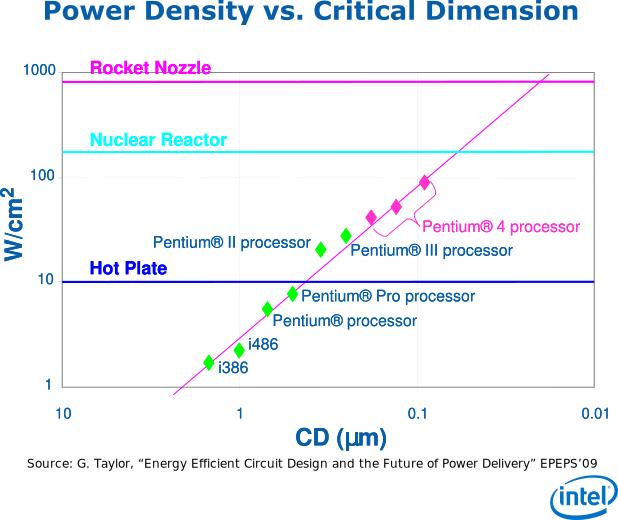
\includegraphics[width=.5\linewidth,keepaspectratio]{powerDensityVSCriticalDim.svg.png}
  \caption[Comparazione tra la densistà di potenza di alcuni dispositivi tecnologici con dei processori intel rispetto alla loro dimensione critica,
			è possibile notare come la i valori raggiunti da alcuni modelli pentium si avvicinino a quelli di un reattore nucleare]
  \decoRule \label{fig:powerDensityVSCriticalDim}
\end{figure}
%%
\voidLine
%https://en.wikipedia.org/wiki/Processor_power_dissipation
Una buona approssimazione della potenza dissipata da un processore è data da:
$P_{cpu} =  P_{dyn} + P_{sc} + P_{leak}$ dove 
\begin{enumerate}
	\item $P_{dyn}\quad$ modella la dissipazione di energia dovuta all'attività interna dei gate logici della CPU,
	approssimabile con $P_{dyn} = CV^2 f$
	\item $P_{sc}\quad$	 modella la dissipazione di energia 
	dovuta ad un collegamento diretto che si può creare tra la sorgente di energia e il ground durante
	un cambiamento di stato di un gate CMOS
	\item $P_{leak}\quad$ modella le perdite di energia intrinseche dei singoli transistors.
\end{enumerate}
Dato che la frequenza di lavoro dell'unità di calcolo è proporzionale ai punti 1 e 2,
è necessario limitarla, purtroppo, per evitare un surriscaldamento critico dei componenti elettronici.\\
Indirettamente, questo comporta la necessità di limitare anche le potenzialità offerte da 
una singola unità di calcolo.
\voidLine
La soluzione per far fronte a questa limitazione fisica/tecnologica e 
fabbricare processori più performanti è quella di realizzare CPU con diverse unità di calcolo separate o core.\\
%SW parallelo che sfrutti i diversi core
In questo contesto si inserisce il calcolo parallelo, ovvero tecniche per realizzare software che 
sfrutti la disponibilità dei vari core del calcolatore mediante un partizionamento del lavoro in parti
assegnabili alle singole unità di calcolo.\\
%TODO HPC in generale... ===> targets, ... TODO ?
\voidLine
%\subsection{High Performance Computing}
L'High Performance Computing si riferisce a tecnologie hardware e software 
usate per realizzare sistemi di elaborazione ad alte prestazioni 
per applicazioni che richiedono computazioni molto onerose, non risolvibili con sistemi informatici tradizionali.\\

\section{Uso di Metodi basati su Algebraic Multi Grid nel calcolo scientifico}
Applicazioni HPC tipiche sono provenienti dal mondo ingegneristico e dal calcolo scientifico,
come ad esempio la risoluzione di equazioni differenziali alle derivate parziali (\emph{PDE}) su dominii 2D o 3D.\\
Le PDE sono usate per descrivere moltissimi fenomeni fisici relativi alla
dinamica dei fluidi, alla meccanica quantistica e chimica computazionale % e molti altri derivanti da applicazioni ingegneristiche, %TODO MORE
così come vari problemi nell'area dell'ingegneria, biologia e economia.\\
Dato che molto spesso non esistono soluzioni esplicite in forma chiusa a queste equazioni,
vengono calcolate soluzioni approssimante ottenute da tecniche numeriche.\\ 
Molte tecniche numeriche per risolvere delle PDE trasformano le equazioni differenziali
in equazioni algebrice, mediante un processo di discretizzazione delle equazioni nel dominio del problema da risolvere.
Conseguentemente un problema ricorrente in varie applicazioni algebriche e nel calcolo scientifico in generale, 
%come gia menzianto %in \ref{chIntro:},
è risolvere sistemi sparsi di dimensioni grandi derivanti da metodi di risoluzione numerici di PDE.\\
\voidLine
Il sistema lineare sparso di riferimento che verrà usato nel seguito è 
\begin{equation} \label{eq:1}
Ax=b
\end{equation}
dove $A$ è una matrice sparsa di grandi dimensioni,
simmetrica e definita positiva \emph{s.p.d.}\\
\subsection{Importanza della sparsità delle matrici}
%sparsity defs
La proprietà di sparsità della matrice $A$ in \ref{eq:1}, ovvero la proprietà di avere per la maggioranza degli elementi il valore zero,
%Since differential surface properties are defined locally, the discretization of PDEs typically leads to sparse linear systems, in which the ith row contains non- zeros only in those entries corresponding to the geodesic or topological neighbor- hood of vertex xi . We are therefore interested in solvers that exploit this sparsity in order to minimize both memory consumption and computation times. 
deriva dalla discretizzazione delle PDE nel problema originario in una mesh di punti \cite{sparseLinearSolverTR}.
Una caratteristica comune nei metodi di discretizzazione utilizzabili come differenze finite, elementi finiti e volumi finiti \cite{spMVfanf,pdeSparsfd1,pdeSparsfd2,pdeSparsfd3}
è che il numero di elementi in ogni equazione discretizzata dipende da proprietà topologiche locali alla discretizzazione
e non dalla dimensione globale del dominio del problema da risolvere. Conseguentemente la matrice generata da questi metodi è comunemente sparsa.
\voidLine
La proprietà di sparsità di $A$ consente l'utilizzo di rappresentazioni idonee in memoria durante il calcolo, 
dove vengono salvati solamente gli elementi \nnz.\\
Formati tipici di memorizzazione per matrici sparse sono: \emph{CompressedSparseColumn, CompressedSparseRow, Ellpack, DIA}.\\
\voidLine	%sparsity advantage
Sfruttare la sparsità delle matrici nella risoluzione consente di ottenere svariati vantaggi
rispetto ad usare le tecniche convenzionali dell'algebra lineare densa, come un utilizzo molto più efficiente della memoria.\\
Spingendo al limite le potenzialità dei super calcolatori attuali e cercando soluzioni sempre più accurate ai problemi moderni di calcolo scientifico,
si rende indispensabile sfruttare questa proprietà quando presente,
dato che tecniche classiche per matrici dense necessiterebbero di una quantità di memoria 
quadratica nella dimensione della matrice, contro una quantità lineare nel numero dei non zeri con tecniche di algebra sparsa.
\voidLine	%prefer of iterative solver to keep sparsity
\subsection{Tecniche risolutive efficienti di sistemi sparsi}
Solutori per problemi del tipo \ref{eq:1}, possono essere di tipo diretto o iterativo.\\
Solutori di tipo diretto tipicamente impiegano una fattorizzazione della matrice $A$ 
in matrici di struttura semplice (triangolare, diagonale, ortogonale) 
per poi applicare operazioni che portano alla soluzione del sistema $x^{\ast}$.\\
Solutori di tipo indiretto generano una sequenza di soluzioni intermedie,
(ipoteticamente) %TODO
convergenti alla soluzione del sistema $x^{\ast}$.\\
Una differenza significativa tra le due classi di soluzioni 
è che i solutori diretti non sfruttano la sparsità della matrice in input
nei passaggi intermedi.
Infatti, in varie misure in base al metodo di risoluzione diretto utilizzato,
la fattorizzazione della matrice può perdere la proprietà di sparsità e divenire densa
come mostrato dalla figura \ref{fig:Efficient_Linear_System_Solvers_for_Mesh_Processing_densificationByDirectSolver}.\\
\begin{figure}[h!]
  \centering \includegraphics[height=.57\columnwidth,keepaspectratio]{Efficient_Linear_System_Solvers_for_Mesh_Processing_densificationByDirectSolver.svg.png}
  \captionsetup{singlelinecheck=off}
  \caption[]{	Varie fattorizzazioni di una matrice altamente sparsa A 500x500 con soli 3502 elementi \nnz (in alto a sinistra)
				in  matrici con un numero di \nnz incrementato a vari livelli:
				\begin{itemize}
					\item	36000 \nnz con il metodo di \emph{Cholesky} in alto a destra
					\item	14000 \nnz con il metodo di \emph{Cuthill-McKee}
					\item	 6203 \nnz con il metodo \emph{minimum degree ordering}
					\item	 7142 \nnz con il metodo \emph{nested dissection method}
				\end{itemize}
				\cite{sparseLinearSolverTR}
  }
  \decoRule \label{fig:Efficient_Linear_System_Solvers_for_Mesh_Processing_densificationByDirectSolver}
\end{figure}
%Fig. 2. The top row shows the non-zero pattern of a typical 500 × 500 matrix A and its Cholesky factor L, corresponding to a Laplacian system on a triangle mesh. Although A is highly sparse (3502 non-zeros), the factor L is dense (36k non-zeros). The reverse Cuthill-McKee algorithm minimizes the envelope of the matrix, resulting in 14k non-zeros of L (2nd row ). The minimum degree ordering avoids fill-in during the factorization, which decreases the number of non-zeros to 6203 (3rd row ). The last row shows the result of a nested dissection method (7142 non-zeros), that allows for parallelization due to its block structure. 
Di contro a questa penalità dei solutori diretti, c'è il vantaggio che la fattorizzazione della matrice $A$, 
può essere riutilizzata per sistemi in cui viene cambiato il lato destro di \ref{eq:1},
%o anche in caso in cui la matrice $A$ cambia i valori \nnz ma non il loro pattern di sparsità... 50% del tempo
come analizzato in \cite{sparseLinearSolverTR}.\\
\voidLine
\subsection{Solutori MultiGrid}
Tra i solutori iterativi più efficienti ci sono quelli basati su metodi \emph{MultiGrid}, 
che godono di ottime caratteristiche di scalabilità come avere un numero di iterazioni e 
un costo per iterazione approssimatamente costante all'incrementare della dimensione del problema \cite{AMGgeneralANY,Sp3MM4AMG}.\\
%MultiGrid in generale-wikipedia
L'idea principale dei metodi MultiGrid è quella di 
risolvere il sistema \ref{eq:1} iterativamente, applicando una serie di correzioni 
alle soluzioni approssimate ottenute con un metodo iterativo basico.\\
Le correzioni sono applicate ai residui associati agli errori delle soluzioni approssimate intermedie
risolvendo un sotto problema dell'originale, contente un sottoinsieme delle incognite. %, a grana meno fine
Il sotto problema può essere risolto a sua volta applicando ricorsivamente delle correzioni
a dei sotto problemi ulteriori, sempre più piccoli e facili da risolvere,
fino a quando la risoluzione dell'ultimo sotto problema è di una difficoltà trascurabile 
rispetto a generarne un altro.\\
%tipi di shape per iterazioni
Le iterazioni di questi metodi possono essere strutturate con cicli di varia natura.
Tra le metodologie principalmente utilizzati ci sono cicli a forma V,F e W.\\
%In figura \ref{fig:Multigrid_Visualization_wikipedia} è disponibile una rappresentazione schemativa di un algoritmo MultiGrid iterativo con un ciclo-V.
\begin{figure}[h!]
  \centering \includegraphics[width=.44\linewidth,keepaspectratio]{Multigrid_Visualization_wikipedia.png}
  \caption[Rappresentazione grafica di un ciclo V di un solutore MultiGrid]
  \decoRule \label{fig:Multigrid_Visualization_wikipedia}
\end{figure}

%\par\null\par	%GMG vs AMG
Tra i principali tipi di metodi MultiGrid disponibili ci sono quelli di tipo Geometrico \emph{GMG} e quelli di tipo Algebrico \emph{AMG}.
La differenza sostanziale è il modo di determinazione dei sotto problemi intermedi da risolvere ad ogni iterazione.\\
Nei metodi Geometrici, si usa una gerarchia di griglie iterativamente più sparse,%TODO derivate da quella di discretizzazione originale,
derivate da informazioni sulla struttura della griglia di discretizzazione originaria.\\
%One main component of this type of multilevel algorithm is a hierarchy of geomet- ric grids, typically a sequence of nested grids obtained by successive refinement. The resulting algorithms are known as geometric multigrid (GMG) methods. 
%AMG finally!
I metodi Algebrici riescono ad utilizzare unicamente informazioni derivanti dalla matrice associata al sistema da risolvere \ref{eq:1},
pur mantenendo la stessa complessità asintotica dei \emph{GMG}.\\
Questa proprietà dei \emph{AMG}, rende possibile applicarli a problemi con una griglia di discretizzazione sottostante non strutturata, come ...
\cite{AMGgeneralANY}.\\
\par\null\par	%GMG vs AMG
La gerarchia di sotto-problemi intermedi da risolvere ad ogni iterazione con i metodi AMG è derivata dal triplo prodotto di Galerkin:\\
$A_{l+i} = (P_l)^T \cdot A_l \cdot P_l~l=0,\dots,nl-1$, dove $A_0 = A$ \cite{amgProf}
e $P_l$ è una sequenza di matrici di prolungamento $n_l x n_{l+1}$ con $n_0=n~n_{l+1}<n_l$.\\
%TODO more?
\par\null\par
%actual time costs :((( , previous prof notes 
%%Non esattamente: di quale algoritmo iterativo stiamo parlando? 
%% Il triplo prodotto viene eseguito durante la costruzione della gerarchia, non durante la applicazione della gerarchia stessa all'interno dell'algoritmo iterativo di soluzione del sistema lineare.
%%E tuttavia, il triplo prodotto è importante perchè il tempo di costruzione del precondizionatore ne dipende. 
%%In generale, il tempo complessivo per un sistema lineare vale 
%%T_{tot} = T_{setup} + T_{it}\times N_{it} 
%%ed il triplo prodotto entra nel tempo di setup. 
%%Se un sistema  con la stessa matrice viene risolto più volte, il precondizionatore si riutilizza, e quindi il tempo di setup viene ammortizzato su più esecuzioni, il che vuol dire che ci si può permettere un setup più complesso.
In generale il tempo complessivo di risoluzione del sistema lineare è $T_{tot} = T_{setup} + T_{it}\times N_{it}$,
dove $T_{it}\times N_{it}$ è associato al costo delle iterazioni del metodo, 
mentre $T_{setup}$ comprende il calcolo di tutto il necessario all'esecuzioni delle iterazioni,
tra cui la costruzione della gerarchia di sotto problemi mediante il triplo prodotto.\\ %TODO setup of preconditioner https://en.wikipedia.org/wiki/Preconditioner#Description ?? 
\par\null\par
Realizzare il triplo prodotto tra matrici sparse,in gergo \emph{Sp3MM: Sparse Triple Matrix Multiplication},  
in parallelo è l'obbiettivo di questa tesi, al fine di potenziare progetti come \cite{AMG4PSBLAS} che sfruttano solutori basati su AMG.\\
%organizzazione seguito
%Il seguito della tesi è strutturato come segue
\section{Algebraic MultiGrid for Parallel Sparse BLAS}
PSBLAS è una libreria software che punta a consentire la realizzazione di varie applicazioni di calcolo scientifico computazionalmnte intense,
mediante implementazioni di risolutori iterativi per sistemi lineari sparsi 
usando il padarigma di programmazione per sistemi a memoria distribuita.\\
L'ambito di questa libreria è applicabile alle PDE discretizzate mediante differenze finite o elementi finiti,
ma anche a problemi di ottimizzazione non lineare come problemi di controllo ottimo \cite{PSBLAS3man}.\\
AMG4PSBLAS \cite{AMG4PSBLASman} fornisce i metodi MultiGrid di tipo algebrico precedentemente descritti,
utilizzando come layer sottostante PSBLAS.\\
Il progetto Software è scritto in Fortran 2003, sfruttandone le possibilità di 
usare un design object-oriented mediante varie funzionalità disponibili nello standard del linguaggio,
consentendo un'ottima gestione delle varie implementazioni offerte. 
				%HPC context (poco poco), pdeDiscretized -> psBlas -> amg4psblas -> criticità prodotto -> ottimizzazione
\chapter{Algoritmi per SpMM esistenti}
\label{ChExistingTecqs}
%----------------------------------------------------------------------------------------



\section{Notazione}	\label{notazione}
Nel seguito si utilizzerà la seguente notazione.\\
Considerando il prodotto tra 2 matrici sparse, si indicherà con $C \in \mathbb{R}^{m x n}$ il risultato del prodotto delle matrici sparse 
$A \in \mathbb{R}^{m x k},B \in \mathbb{R}^{k x n}$. Dove:\\ 
$a_{ij} \in A$ è l'elemento della riga i e colonna j della matrice A.\\
$a_{i*}~,~a_{*j}$ indicano rispettivamente la riga i-esima e la colonna j-esima della matrice A\\
$a_{i~c_z-c_w} = \left\{ a_{ij} \in a_{i*} :~ j \in [c_z,c_w] \right\}$  
indica la partizione delle colonne nel range $[c_z,c_w]$ della riga i-esima della matrice A.\\

$I_i(A)$ indica il set di indici di colonna relativi agli elementi \nnz della riga i-esima di A\\
$I^j(B)$ indica il set di indici di riga relativi agli elementi \nnz della colonna j-esima di B\\
$I(i,j)$ indica il set di indici $k$ di righe di A e di colonne di B tali che
$a_{ik}*b_{kj} \neq 0$\\
$nnz(A)$ indica il numero di non zeri della matrice A. \\ 
$nzc(A)~,~nzr(A)$ indicano rispettivamente il numero di colonne e di righe di A con almeno un elemento \nnz\\
$\hat{C}$ indica una struttura contenete risultati intermedi al prodotto $A \cdot B$.\\

\label{notazioneSp3MM}
Considerando invece il prodotto tra 3 matrici sparse, %ad esempio in applicazione di AlgebraicMultiGrid,
si indicherà con $AC_{i+1} \in \mathbb{R}^{n_{i+1} x n_{i+1} }$ il risultato del triplo prodotto tra le seguenti matrici in quest'ordine
$R \in \mathbb{R}^{n{i+1} x m} ~  AC_i \in \mathbb{R}^{n^i x n^i} ~ P \in \mathbb{R}^{m x n^{i+1}}$, dove $i~<~i+1$.\\

\label{notazioneNaming}
%TODO indici <-> indici degli elementi \nnz 
Con Sp3MM si indicherà il triplo prodotto tra matrici sparse: $AC_{i+1}=R \cdot AC_i \cdot P$
Con moltiplicazione scalare si intenderà il prodotto tra uno scalare $a \in \mathbb{R}$ per un vettore $v \in \mathbb{R}^n$\\

\section{Formulazioni SpMM}	\label{ChExistingTecqs:formulazioni}
Gli algoritmi per la risoluzione del prodotto tra due matrici sparse possono
essere classificati in base alle formulazioni e partizionamento dei dati del problema SpMM 
\cite{sysReviewChi}.\\ Le principali formulazioni del problema sono sono:
\begin{itemize}
  \item Inner-product \qquad $c_{ij} = \sum\limits_{k \in I(i,j)}  a_{ik} \ast  b_{kj}$
  \item Outer-product \qquad $C = \sum\limits_{i=1}^k  a_{*i} \otimes  b_{i*}$		
  \item row-by-row	  \qquad $c_{i*} = \sum\limits_{k \in I_i(A)}  a_{ik} \ast  b_{k*}$
  \item col-by-col    \qquad $c_{*j} = \sum\limits_{k \in I^j(B)}  a_{*k} \ast  b_{kj}$
\end{itemize}

\subsection{Rappresenzione mediante grafi}
Le formulazioni per MM possono essere rappresentate graficamente mediante
grafi a 3 strati U, W, V \cite{2dNewIdeas,cohen3LayeredGraphs} dove:
\begin{itemize}
  \item i nodi in $U \ni u_i$:   rappresentano le righe di A
  \item i nodi in $V \ni v_j$:   rappresentano le colonne di B
  \item i nodi in $W \ni w_k$:   rappresentano la dimensione in comune tra A e B
\end{itemize}
esiste un arco $(u_i,w_l) ~ \forall ~ a_{i,l} \neq 0$\\
esiste un arco $(w_l,v_j) ~ \forall ~ b_{l,j} \neq 0$\\
%%TARGET GRAPH RAPPR
Per ogni formulazione di SpMM, l'obbiettivo è quello di trovare coppie di
vertici $(u_i,v_j)$ connessi da un nodo comune $w_k$ e unire i
contributi di coppie di vertici che condividono nodi adiacenti\\ %TODO

%%INNER PRODUCT
\begin{figure}[h!]
  \centering \includegraphics{layeredGraphInnerProduct.svg.png} 
  \caption[Rappresentazione grafica del calcolo di $c_{i,j}$ mediante Inner-product]
  \decoRule \label{fig:layeredGraphInnerProduct}
\end{figure}
Per la formulazione Inner-product \ref{fig:layeredGraphInnerProduct} 
è necessario esaminare ogni coppia di vertici  in U e V per trovare 
il sottoinsieme di $\tilde{W_{ij}} \subseteq W$ che connette coppie di nodi. \\
Vengono accumulati i prodotti $a_{il} \cdot b_{lj}$ relativi a $\tilde{W_{ij}}$ in $c_{ij}$.\\
È possibile osservare come la sparsità delle matrici non è sfruttata dato
che è necessario analizzare tutte le coppie di nodi $(u_i,v_j)$\\
%%OUTER PRODUCT
\begin{figure}[h!]
  \centering 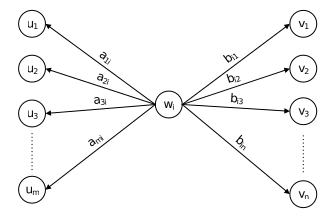
\includegraphics{layeredGraphOuterProduct.svg.png} 
  \caption[Rappresentazione grafica della componente $a_{*i} \cdot b_{i*}$ del calcolo di C mediante Outer-product]
  \decoRule \label{fig:layeredGraphOuterProduct}
\end{figure}
Per la formulazione Outer-product \ref{fig:layeredGraphOuterProduct}
è possibile identificare le coppie di vertici connesse a
partire dai nodi di W che, per matrici sufficientemente sparse,
può essere un'operazione più veloce rispetto all'Inner-product.\\
%TODO si complica l'accumulazione dei risultati intermedi
%%row-by-row
\begin{figure}[h!]
  \centering 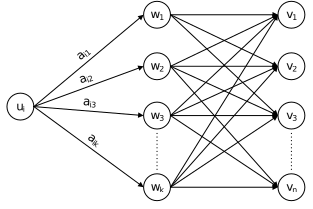
\includegraphics{layeredGraphRowByRow.svg.png} 
  \caption[Rappresentazione grafica della componente $a_{i*} \cdot B$ del 
     calcolo di C mediante formulazione row-by-row]
  \decoRule \label{fig:layeredGraphRowByRow}
  
\end{figure}
Per la formulazione Row-by-row \ref{fig:layeredGraphRowByRow}
le coppie di vertici d'interesse per il risultato di C sono identificabili 
a partire da attraversamenti del grafo indipendenti a partire dai vertici di U verso V.\\
%%col-by-col
Nel caso col-by-col vi è un attraversamento del grafo dai nodi di V a U, 
isomorfico rispetto al caso Row-by-row\\


\section{Determinazione della dimensione matrice risultante} \label{ChExistingTecqs:symbMul}
Una caratteristica comune degli algoritmi per la moltiplicazione parallela di matrici sparse è 
quella di preferire pre-allocazioni per $C$ e $\hat{C}$ 
invece di usare (ri)allocazioni dinamiche durante la computazione parallela del prodotto.\\
È possibile giustificare questa tendenza considerando genericamente algoritmi paralleli implementati con 
\label{ChExistingTecqs:openMP_for_philosophy}
direttive OpenMP come \verb|#pragma omp parallel for|, che permettono di effettuare una 
parallelizzazione di cicli, noto precedentemente il numero di iterazioni da suddividere tra i thread. \\
In questo contesto, allocazioni dinamiche richiedono la possibilità di poter uscire precedentemente dal ciclo parallelizzato
data la possibilità di fallimento di una (ri)allocazione, il che è contrario alla filosofia di parallelizzazione OpenMP
(per quanto siano disponibili costrutti per una uscita anticipata, che però richiedono una speciale configurazione, disabilitata di default per 
 motivi di performance \ref{ompSpec} )\\
Si considereranno quindi solo implementazioni per SpMM che richiedono il numero di \nnz di $C$ e $\hat{C}$ per 
effettuarne una pre-allocazione.\\

Il numero di \nnz delle righe del risultato dell'operazione di SpMM può essere determinato:\\ %%TODO bigO costs add?
sia con un UpperBound con un basso costo computazionale \\ %O(A.NZ * 2 ) accesso elemento + accesso B.IRP riga corrispondente
sia con in una modalità accurata con maggiore costo computazionale.\\ %[RBtree] || IDXMAP O(A.NZ * B.maxRowLen [* log(A.maxRowLen*B.maxRowLen)] );

\label{ChExistingTecqs:spMM_symb_num_naming}
Il calcolo (di un bound superiore) del numero di numero di \nnz di $C$ e $\hat{C}$ viene tipicamente 
denominato Prodotto Simbolico o fase simbolica, 
viceversa il calcolo effettivo dei \nnz invece Prodotto Numerico o fase numerica.\\

\subsection{UpperBound}	\label{ChExistingTecqs:symbUpperBound}
Un UpperBound sulla lunghezza di una riga risultante a SpMM è computabile come riportato nell'algoritmo 4 di \cite{sysReviewChi}.\\
In questa soluzione, ispirandosi a una formulazione row-by-row di SpMM, 
si determina la dimensione massima di ogni riga della matrice risultante come:\\
$ | I_i(C) |~\leq~\sum\limits_{ j \in I_i(A) }  | I_j(B) | $.\\
Nel caso di allocare la matrice mediante UpperBounds, è necessario effettuare anche una operazione di copia finale,
per riordinare le righe o raccoglierne i \nnz prodotti nella matrice risultate all'operazione di SpMM.\\

\subsection{Prodotto Simbolico Accurato}
L'operazione di determinare esattamente la dimensione della matrice prodotta da SpMM
è denominata in vari articoli Prodotto Simbolico e 
la seguente operazione di moltiplicazione dei vari elementi non zero è denominata Prodotto Numerico.\\

Un approccio tipico per determinare la dimensione di una riga risultante al operazione di SpMM, 
è quella di mantenere in una struttura di ricerca gli indici corrispondenti 
ai \nnz risultanti alle operazioni di prodotto, senza effettuare le costose 
operazioni di moltiplicazione floating point tra gli elementi non zero.\\
%TODO ad esempio come riportato in \ref{RITROVA ARTICOLO CHE DESCRIVE IL PRODOTTO SIMBOLICO}

\section{Algoritmi}
%%SRC STUDIES = Gustavson
Molte delle ricerche riguardo SpMM sono basate sull'algoritmo di Gustavson \cite{gustavson},
un algoritmo sequenziale basato sulla formulazione Row-by-row, riportate in forma di pseudo-codice 
in \ref{figCode:gustavsonRigheSysSurvey} e graficamente in \ref{fig:gustavsonRigheGraphicalIntel}.\\

\begin{figure}[h!]
  \caption[pseudo-codice dell'algoritmo di Gustavson]
  \centering 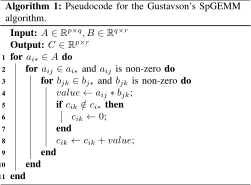
\includegraphics{gustavsonRigheSysSurvey.svg.png} \decoRule
  \label{figCode:gustavsonRigheSysSurvey}
\end{figure}
\begin{figure}[h!]
  \caption[rappresentazione grafica di una iterazione dell'algoritmo di Gustavson]
  \centering 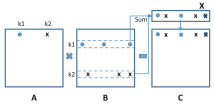
\includegraphics{gustavsonRigheGraphicalIntel.svg.png} \decoRule
  \label{fig:gustavsonRigheGraphicalIntel}
\end{figure}
È possibile notare come nell'algoritmo vi sia l'esigenza di accumulare le righe
risultanti della matrice C. Meccanismi efficienti per realizzare questa
funzionalità sono analizzati successivamente in \ref{ssec:gustavsonDerivate} %TODO FIX REF
\\


\section{Algoritmi paralleli con formulazione multidimensionale} 
Gli algoritmi paralleli risolutivi del prodotto tra matrici possono essere
classificati in base al partizionamento del carico di lavoro sui processi.\\
\begin{figure}[h!]
  \centering \includegraphics{pMM_cube.svg.png} 
  \caption[Rappresentazione grafica dell'assegnamento dei task per la risoluzione
      di SpMM in 1,2 e 3 dimensioni]\decoRule \label{fig:pMM_cube}
\end{figure}
%%WORKCUBE INTRO
L'assegnamento dei sotto problemi può essere visualizzato in un cubo di lavoro W \ref{fig:pMM_cube}
in cui ogni moltiplicazione di elementi \nnz $a_{i,k}*b_{k,j}$ è rappresentabile
con voxel $W(i,j,k)$ \cite{cartesianPartitioningModels}.
Le proiezioni $W(i,j,k)$  sulle facce del cubo relative alle matrici A e B 
hanno elementi \nnz e determinano il pattern degli elementi \nnz sulla matrice C.
%WORKCUBE NOTATIONS
\label{ChExistingTecqs:workCube}
I sottoinsiemi dei voxel di W ottenuti fissando uno o due indici sono denominati:
\begin{itemize}
  \item Layers: W(i,:,:),W(:,j,:),W(:,:,k)
  \item Fibers: Intersezioni di Layers relativi a indici diversi, e.g. W(i,j,:)
  \item Cuboid: Sottoinsiemi di W con tutte le dimensioni minori delle 
   dimensioni delle matrici corrispondenti
\end{itemize}

\subsection{Matrici ipersparse e rappresentazione DCSC}
È possibile definire una matrice sparsa A, come {\bf ipersparsa }se $nnz(A)$ è
inferiore alla sua dimensione più grande N \cite{2dNewIdeas} \\ %TODO newIdeas 14.2.2 x matrici quadrate
Tipicamente questa tipologia di matrici è rara nell'algebra lineare numerica.
Infatti, nella soluzione di sistemi lineari, le matrici sono quadrate, ed avere un numero di nonzeri inferiore alla dimensione 
vorrebbe dire che alcune equazioni non hanno coefficienti, 
il che nei problemi provenienti da equazioni differenziali chiaramente non ha senso.
Tuttsvia, questa tipologia di matrici trova applicazioni nel partizionamento di matrici sparse 
e nel processamento grafi, particolarmente se in parallelo.\\

Data una suddivisone bidimensionale di una matrice sparsa, %TODO quadrata
per un processamento parallelo in una griglia di p processi, si ha che ogni processo
verrà assegnato ad una matrice di dimensione circa $(n/\sqrt{p})~x~(n/\sqrt{p})$. %TODO ~~
L'occupazione globale di spazio di memoria sarà pari a 
$O(nnz + p \cdot n/\sqrt{p}) = O(nnz + n \cdot \sqrt{p})$ con CSC che è maggiore
dell'occupazione totale della matrice in un singolo processo $O(n + nnz)$.\\
Allo scalare del numero di processi p, il termine $n\sqrt{p}$ domina $nnz$.\\
%TODO The ineffciency of CSC leads to a more fundamental problem: any algorithm that
%uses CSC and scans all the columns is not scalable for hypersparse matrices. 
%Even without any communication at all, such an algorithm cannot scale for $n\sqrt{p} > \max{flops,nnz}$

Per queste ragioni è possibile utilizzare la rappresentazione \\
{\bf D}ouble{\bf C}ompressed{\bf S}parse{\bf C}olumns,\ref{fig:DCSCvsCSC}
che ha un'occupazione di memoria pari ad $O(nnz)$
eliminando eventuali ripetizioni nell'array di puntatori delle colonne (JC) nel formato CSC.
È possibile favorire un rapido accesso alle colonne della matrice mediante un
array ausiliario di indici delle colonne \nnz
%TODO qualche spiegazione ulteriore
\begin{figure}[h!]
  \caption[confronto delle rappresentazioni DCSC e CSC ]
  \centering 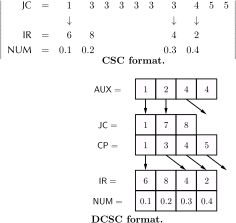
\includegraphics{DCSCvsCSC.svg.png} \label{fig:DCSCvsCSC}
\end{figure}

\subsection{Moltiplicazione tra matrici ipersparse rappresentate con DCSC}
\label{ssec:hypersparseMM}
Segue la descrizione di un algoritmo risolutivo per la moltiplicazione tra matrici
ipersparse \cite{2dNewIdeas}, basato su una formulazione outer-product ed
utilizzato in alcuni algoritmi SpMM.\\
lo pseudo-codice dell'algoritmo è riportato in \ref{figCode:hypersparseMM} 


{\bf fase di preprocessamento} \\
viene effettuata una trasposizione di B, così da avere un indicizzamento rapido delle righe di B
in formato DCSC, necessario per la
formulazione outer-product.\\ 
%costo di trasposizione varia tra $O(n + nnz(B) \to nnz(B) lg nnz(b)) in base all implementazione
Viene effettuata l'intersezione tra gli indici delle colonne non zero di A e
delle righe non zero di B, identificando così il set $Isect = A.JC \cap B^T.JC$ degli
indici che partecipano all'outer-product.\\
\\
Successivamente vengono effettuati $|Isect|$ prodotti cartesiani \ref{fig:hypersparseMMGraphical} 
generanti matrici $a_{*i} \cdot b_{i*}$, i cui elementi è possibile mettere in biiezione 
con la lista di indici $(r_{id},c_{id})$ derivante dal prodotto cartesiano tra gli indici
di riga non zero della colonna i-esima di $B^T$ e gli indici di riga non zero 
della colonna i-esima di $A$.\\
La matrice risultante C può essere ottenuta mediante l'unione di queste liste,
sommando i contributi degli elementi aventi gli stessi indici in liste
diverse.\\
Per implementare la costruzione di C dagli outer-products
è utilizzata una coda con priorità contenete elementi relativi ai
prodotti cartesiani per le colonne di $A$ e le colonne di $B^T ~\in~ Isect$, 
aventi per chiave $(r_{id},c_{id})$ e per valore il prodotto relativo e l'indice
della colonna di $A$ o $B^T$ relativa.\\
Verrà ripetutamente estratto il minimo dalla coda e reinserito
l'elemento successivo dalla lista di indici di relativa, sommando i
contributi di elementi con la stessa chiave.
I risultati verranno accumulati in uno stack mediante una rappresentazione
matriciale a coordinate degli elementi % TODO CHECK COO LIKE STACK ACCUMULATE
per poi essere convertiti nella matrice finale C in formato DCSC.\\

La complessità computazionale dell'algoritmo è $O(nzc(A) + nzr(B) +flops \cdot lg( ni))$
dove $ni$ è la dimensione della coda con priorità e $flops$ è il numero di
operazioni aritmetiche necessarie per il prodotto di A e B.\\

\begin{figure}[h!]
  \centering 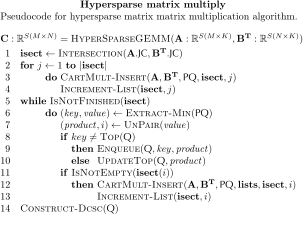
\includegraphics{hypersparseMM.svg.png}
  \caption[Algoritmo sequenziale per SpMM tra matrici ipersparse] \decoRule \label{figCode:hypersparseMM}
\end{figure}

\begin{figure}[h!]
  \centering \includegraphics{hypersparseMMGraphical.svg.png}
  \caption[Rappresentazione grafica del prodotto cartesiano 
   a supporto di hypersparseMM ] \decoRule \label{fig:hypersparseMMGraphical}
\end{figure}


\subsection{Algoritmi con un partizionamento 2D}

\subsubsection{Derivati di Gustavson} \label{ssec:gustavsonDerivate}
Una parallelizzazione della formulazione per righe dell'algoritmo di Gustavson è
descritta in \cite{intelSpMMDenseAccumulator}, sfruttando la
rappresentazione di matrici sparse in formato CSR.  \label{ssec:intelSpMMDenseAccumulator}
Lo pseudocodice dell'algoritmo è riportato in \ref{figCode:gustavsonRigheBlocksIntel}
e una sua rappresentazione grafica è raffigurata in
\ref{fig:gustavsonRigheBlocksGraphicalIntel}\\
%Partizionamento = Gustvason a blocchi
Viene effettuato un partizionamento delle righe di A e delle colonne di B e 
coppie di partizioni corrispondenti vengono utilizzate per calcolare un
blocco bidimensionale della matrice risultante C.\\
%accumulatore denso X
In accordo con la formulazione per righe dell'algoritmo di Gustavson, vengono
accumulati i contributi degli elementi \nnz delle righe di A e corrispettive porzioni
delle righe di B relative al calcolo di un blocco di C. 
Per effettuare efficientemente questa operazione, i vettori sparsi risultanti
dalle iterazioni dell'algoritmo, vengono accumulati in vettore denso X, 
semplicemente sommandone le componenti \nnz nelle relative locazioni di X.\\
%alternative memory efficient con overhead
In questa formulazione del problema, una soluzione di accumulazione 
alternativa potrebbe essere quella di accumulare i contributi per una riga di C 
utilizzando una hash-table di elementi aventi per chiave l'indice di colonna. 
Tuttavia, quest'approccio ha lo svantaggio di avere l'overhead relativo alla 
computazione delle funzioni hash e gestione di eventuali liste di collisione.\\
%implementazione conversione
Al termine del calcolo di una riga di un blocco di C, l'accumulare X viene
convertito in una riga CSR con l'ausilio di un ulteriore vettore di indici di
elementi \nnz sommati in X.\\
%Nota su partizionamento -> MENO cache miss su X
Utilizzando un partizionamento delle colonne di B è possibile partizionare anche
l'accumulatore X relativo ad una riga risultante di C. In questa maniera si
riduce il numero di cache line toccate dagli aggiornamenti di X, riducendo il
numero di cache miss relativi al ciclo interno dell'algoritmo.\\
Gli autori dell'algoritmo hanno verificato la riduzione di cache miss
utilizzando degli hardware counter per verificare il numero di cache miss L2
(tipicamente catturati dalla cache LLC) al variare del partizionamento di B % TODO QUANTIFICAZIONE?
%%Valutazione sul partizionamento di B -> X
%svantaggi
Tuttavia il partizionamento di B in rappresentazioni CSR separate, 
oltre che comportare un overhead computazionale, può comportare svantaggi in
termini di banda di memoria durante la lettura dei blocchi di B, che possono
essere notevolmente più sparsi della matrice originaria. %TODO link a ipersparse
%quantificazione euristica beneficio
Un beneficio dal partizionamento di B e di X, contro gli overhead citati, è
presente quando si ha certezza che per una significativa porzione delle righe
risultanti di C, l'occupazione dei non zeri, corrispondenti agli aggiornamenti
dell'accumulatore X, è maggiore della dimensione della cache L2.\\
Per quantificare il numero di \nnz nelle righe risultanti di C viene utilizzata
una metrica basata sulla stima di \nnz in $c_{i*}=e\_nnz(i)$ di
\cite{intelSpMMDenseAccumulator} %TODO SOURCE ARTICLE OF ESTIMATE
dove si partiziona B se
$e\_nnz = \frac{\sum\limits_{i:e\_nnz(i) > L2\_FP\_WORDS} e\_nnz(i)}
{\sum\limits_{i=1}^m e\_nnz(i)} ~>~0.3$\\
%TODO scheduling dinamico -> load balancing con perizioni piccole t.c. #partizioni = 6-10 X #threads
\begin{figure}[h!]
  \centering 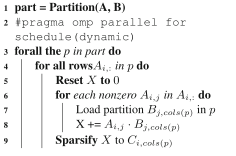
\includegraphics{gustavsonRigheBlocksIntel.svg.png}
  \caption[adattamento parallelo dell'algoritmo di Gustavson] \decoRule \label{figCode:gustavsonRigheBlocksIntel}
\end{figure}
\begin{figure}[h!]
  \caption[rappresentazione grafica dell'adattamento parallelo dell'algoritmo di Gustavson] 
  \centering \includegraphics{gustavsonRigheBlocksGraphicalIntel.svg.png} \label{fig:gustavsonRigheBlocksGraphicalIntel}
\end{figure}

L'uso di un vettore denso per operazioni tra matrici sparse è stato 
affrontato originariamente da \cite{SPA_mathlab}.\\

\subsubsection{Dense SUMMA} %versione base C=AB
Un partizionamento bidimensionale della risoluzione del prodotto tra matrici
dense è realizzato dell'algoritmo parallelo SUMMA \cite{denseSumma} che è alla
base di una sua controparte per matrici sparse \cite{sparseSUMMA}.\\
Il calcolo di $C=AB$ è suddiviso in sottomatrici assegnate a processi organizzati 
in una griglia bidimensionale di dimensione  $p_r x p_c$.\\
È possibile calcolare un blocco della matrice C come:
$C_{ij} =  \overbrace{\left(  A_{i1} | \dots |  A_{ip_c} \right)}^{\tilde{A^{i*}} }
~\cdot~ \overbrace{\left( 
        \begin{array}{c} B_{1j} \\ \vdots \\  B_{p_r j}
        \end{array} \right)} ^{\tilde{B^{*j}}} $\\
dove si usa la notazione:
\begin{itemize}
  \item $\tilde{a_{*l}}^{i*} \in \tilde{ A^{i*}}$ rappresenta 
    la colonna l-esima nella riga i-esima nella decomposizione a blocchi di A
  \item $\tilde{b_{l*}}^{*j} \in  \tilde{B^{*j}}$ rappresenta 
    la riga l-esima nella colonna j-esima nella decomposizione a blocchi di B.
\end{itemize}  
Applicando la formulazione outer-product su $\tilde{ A^{i*}}$ e $\tilde{B^{*j}}$
si ha che $C_{ij}=\sum\limits_{l=1}^{k}\tilde{a_{*l}}^{i*} \cdot \tilde{b_{l*}}^{*j}$\\
Considerando un partizionamento delle matrici in sottomatrici all'interno della
griglia di processi %assegnate in maniera tale che  ... 
si può eseguire l'operazione MM in parallelo come riportato dallo pseudocodice
in \ref{figCode:denseSUMMA}\\
\begin{figure}[h!]
  \centering 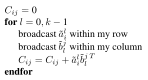
\includegraphics{denseSUMMA.svg.png}
  \caption[esecuzione dense SUMMA sul processo $P_{ij}$] \decoRule \label{figCode:denseSUMMA}
\end{figure}
Nell'articolo originale vengono discussi miglioramenti a questa formulazione
basati su uno scambio di dati tra i processi in un sistema a memoria distribuita
mediante una comunicazione ad anello 
riformulazione del calcolo di $C_{ij}$ utilizzando blocchi di
colonne di $\tilde{ A^{i*}}$ e righe di $\tilde{B^{*j}}$.\\

\subsubsection{Sparse SUMMA}
Un partizionamento bidimensionale del problema SpMM è realizzato
dall'algoritmo Sparse SUMMA \cite{sparseSUMMA}, derivato dalla sua
controparte per matrici dense.\\
%SPARSE SUMMA
È riportato lo pseudo-codice dell'algoritmo sparseSUMMA 
in \ref{figCode:sparseSUMMA} e una sua iterazione graficamente in
\ref{fig:sparseSUMMAIteration}.\\
Le matrici sono divise in blocchi e rappresentante in formato DCSC,
trasponendo la matrice B per avere un indicizzamento rapido delle sue righe.\\
Procedendo in blocchi di colonne di una sottomatrice di A e della corrispettiva
sottomatrice di $B^T$, lungo la dimensione comune di A e B,
vengono calcolati in parallelo le sottomatrici $C_{ij}$, 
utilizzando l'algoritmo hypersparseMM \ref{ssec:hypersparseMM}.\\
Il costo computazionale dell'algoritmo è 
$O(\frac{dn}{\sqrt{p}}+\frac{d^2n}{p}lg(\frac{d^2n}{p}))$
%TODO CONSIDERAZIONE SU EFFICIENZA ALLO SCALARE DI p ... cmq no speedup bounds!
\begin{figure}[h!]
  \caption[SparseSUMMA, per una risoluzione parallela di SpMM con un partizionamento 2D]
  \centering \includegraphics{sparseSUMMA.svg.png} \decoRule \label{figCode:sparseSUMMA}
\end{figure}
\begin{figure}[h!]
  \caption[esecuzione di un iterazione dell'algoritmo sparseSUMMA]
  \centering \includegraphics{sparseSUMMAIteration.svg.png} \decoRule \label{fig:sparseSUMMAIteration}
\end{figure}

\subsection{Algoritmi con un partizionamento 3D}
Un partizionamento tridimensionale del problema SpMM è realizzato dall'
algoritmo Split-3D-SpMM \cite{Split3DSpMM}, dove al partizionamento
bidimensionale descritto precedentemente, viene aggiunto una ulteriore
suddivisione delle sottomatrici in blocchi nella terza dimensione della griglia di processi.
%TODO CONSIDERAZIONI su overhead mem per C -> sparsity-structure dependent ->
%sfruttabile bene la sparsità del risultato in meno occupazione di memoria
Il partizionamento delle matrici è rappresentabile sul cubo di lavoro W come
riportato in figura \ref{fig:workCube3D}, dove il processo P(i,j,k) possiede la
porzione della matrice di A: 
$A(im/p_r:(i+1)m/p_r - 1, jn/p_c + kn/(p_c p_l ) : jn/p_c + (k + 1)n/(p_c p_l) - 1)$  \\
\begin{figure}[h!]
  \caption[rappresentazione 3D della suddivisione della computazione SpMM]
  \centering \includegraphics{workCube3D.svg.png} \decoRule \label{fig:workCube3D}
\end{figure}
L'algoritmo è riportato nello pseudo-codice \ref{figCode:Split3DSpMM} e una
sua iterazione è raffigurata graficamente in \ref{fig:Split3DSpMMIteration}.\\

In maniera simile al caso di sparseSUMMA %TODO \ref{sparseSummaDescriptionStart}
si procede in parallelo calcolando il prodotto di sotto blocchi corrispondenti
alle sottomatrici di A e B, accumulando risultati intermedi la cui collocazione
è relativa all'intera fiber W(i,j,:).
Infine i risultati intermedi dei processi P(i,j,:), vengono distribuiti lungo la fiber
W(i,j,:), sommando i contributi relativi agli stessi indici.
\begin{figure}[h!] 
  \caption[Split3DSpMM, per una risoluzione parallela di SpMM con un partizionamento 3D
     nel caso semplificato di una griglia di processi $\sqrt{p/c}~x~\sqrt{p/c}~x~c$]
  \centering 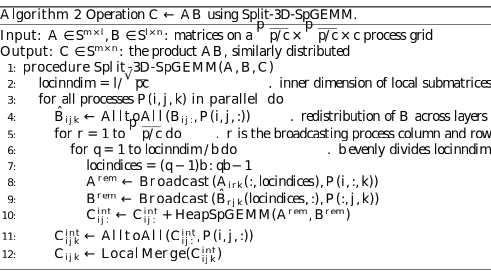
\includegraphics[width=1.0\textwidth]{Split3DSpMM.svg.png} \decoRule \label{figCode:Split3DSpMM}
\end{figure}
\begin{figure}[h!]
  \caption[esecuzione di un iterazione dell'algoritmo Split3DSpMM]
  \centering 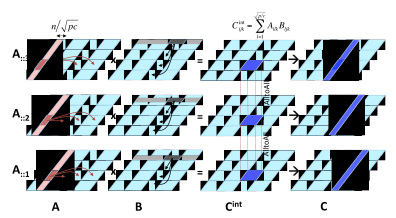
\includegraphics[width=1.0\textwidth]{Split3DSpMMIteration.svg.png} 
  \decoRule \label{fig:Split3DSpMMIteration}
\end{figure}

\section{Algoritmi paralleli basati su formulazione Outer-Product}
%\item Outer-product \qquad $C = \sum\limits_{i=1}^k  a_{*i} \otimes  b_{i*}$		
Implementazioni di SpMM basate su formulazioni di Outer-Product, godono di una
potenziale migliore località spaziale dei \nnz acceduti durante il prodotto,
come spiegato in \cite{ESC}.\\
\label{ChExistingTecqs:gustavsonDerivateBadAccessLocalityNNDominantMatrix}
Considerando rispettivamente formulazioni row-by-row e col-by-col per SpMM e denominando 
la matrice dominante nei prodotti rispettivamente A e B,
si ha una buona località spaziale per le matrici dominanti e risultanti ma non per quelle non dominanti.
Questo è dovuto al fatto che la matrice non dominante deve essere acceduta per righe o colonne 
in un ordine derivato dal pattern di sparsità dei non zeri delle matrici dominanti, che è assimilabile ad un ordine casuale.\\

Nel caso row-by-row ad esempio, si può avere un cattivo uso della cache in scenari dove:\\
una riga di B deve essere riletta varie volte, ma l'ordinamento degli accessi alle righe di B causa
che, il più delle volte, la riga non sia in cache quando necessario.\\
In questi casi si ha che formulazioni row-by-row o col-by-col causano uno spreco di banda di memoria,
il che è particolarmente critico per un problema memory bound come SpMM.\\
%%OuterProduct visual
\begin{figure}[h!]
  \centering 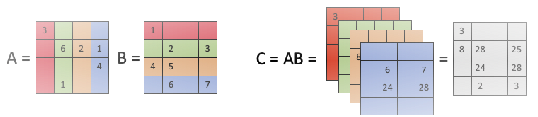
\includegraphics{imgs/outerProductExampleVisual_ESC.svg.png}
  \caption[Visualizzazione di un prodotto tra matrici 4x4 mediante Outer-Product]
  \decoRule \label{fig:outerProductExampleVisual_ESC}
\end{figure}

\subsection{ESC - PropagationBlocking}
Una soluzione per l'operazione di SpMM mediante Outer-Product è riportata in \cite{ESC},
dove viene usato un algoritmo basato sul generale approccio risolutivo Expand-Sort-Compress, %TODO cerca di piu ESC in generale
applicato ad una formulazione Outer-Product per SpMM.\\

Le principali fasi dell'algoritmo sono:
\begin{itemize}
	\item $\hat{C}~\leftarrow~$Symbolic(A,B) \\ Allocazione dei risultati intermedi al prodotto mediante un UpperBound
	\item $\hat{C}~\leftarrow~$Expand(A,B)	 \\ Esecuzione dei prodotti a rango 1 della formulazione Outer-Product in formato COO
	\item Sort($\hat{C}$) 					 \\ Ordinamento mediante radix-sort dei prodotti intermedi mediante le loro coordinate risultanti
	\item $C~\leftarrow~$Compress($\hat{C}$) \\ unione dei risultati intermedi, sommandoli nella matrice finale
\end{itemize}

%%Algo Steps bigPic
\begin{figure}[h!]
  \centering 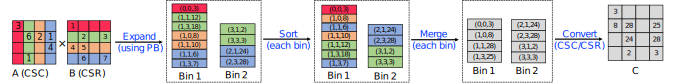
\includegraphics{OuterProduct_PBAlgoritmExample_ESC.svg.png}
  \caption[Rappresentazione grafica degli step principali dell'algoritmo] 
  \decoRule \label{fig:OuterProduct_PBAlgoritmExample_ESC}
\end{figure}

\subsubsection{Symbolic -- UB estimate}
Analogamente a quanto descritto precedentemente in \ref{ChExistingTecqs:openMP_for_philosophy}, 
preferendo una preallocazione delle strutture intermedie necessarie rispetto ad effettuare (ri)allocazioni dinamiche, 
viene calcolata la dimensione dei risultati intermedi che corrisponde ad un UpperBound della dimensione finale del risultato.\\
Seguendo un approccio Outer-Product per SpMM, il numero di \nnz al termine della fase Expand è pari ad:\\
$ \sum\limits_{i = 1}^k  | I^i(A) | *| I_i(B) | $ \\ % flops + = nnz(B(i, :)) × nnz(A(:, i))
 
\subsubsection{Expand}
In questa fase vengono effettuati i prodotti richiesti dalla formulazione Outer-Product, 
salvando i non zeri come tuple con il risultato numerico e le coordinate di righe e colonne (formato COO).\\
Per questioni di efficienza è necessario che la matrice A sia in un formato con colonne contigue (CSC) 
e B in un formato con righe contigue (CSR).\\
Queste tuple vengono generate e raggruppate in parallelo in bin in base agl'indici di riga dei corrispondenti elementi di A.\\
Per una maggiore efficienza ogni thread mantiene una copia locale di tutti i $m$ bin possibili, 
effettuando periodicamente una operazione di \emph{flush} dei dati locali nei bin globali.\\ 

\begin{figure}[h!]
  \centering \includegraphics{OuterProduct_PBAlgo_BinsExample_ESC.svg.png}
  \caption[Rappresentazione grafica delle operazioni di flush periodiche dei bin locali ai thread nei bin globali]
  \decoRule \label{fig:OuterProduct_PBAlgo_BinsExample_ESC.svg.png}
\end{figure}

%PropagationBlocking Explaination ... TODO non menzionato esplicitamente nel paper... interpolato da qua e la xD
Il termine "PropagationBlocking" deriva da questa organizzazione dei prodotti in Bin locali e globali, 
consentendo insieme alle fasi successive una somma efficiente dei valori 
corrispondenti allo stesso elemento \nnz nella matrice risultante.\\

\subsubsection{Sort}
Si effettua un sorting delle tuple prodotte in $\hat{C}$ nei bin globali nella fase precedente,
ordinandole in base ai campi relativi alle coordinate di righe e colonne.\\
Gli autori dell'articolo asseriscono di usare una versione inplace di radix-sort, 
che raggruppa le chiavi in base alla posizione del byte più significativo 
(richiedendo cosi un numero di passate sui dati proporzionale al numero di byte nelle chiavi),
dando performance migliori rispetto ad algoritmi basati su comparazioni per chiavi piccole.\\
Utilizzando un numero di bin tale da averene la maggior parte in dimensione tale 
da poter entrare in cache L2 o L3 è possibile effettuare il sorting in cache, 
attenuando il costo dovuto alle riletture dei dati per l'operazione di ordinamento.

\subsubsection{Compress}
Si sommano tutte le tuple aventi stesse cordinate di riga e colonna, corrispondenti allo stesso elemento non zero
nella matrice risultante.\\
Grazie all'ordinamento effettuato nella fase precedente, è possibile completare questa fase con una singola
scansione di tutti i Bin globali.\\


Per facilitare le fasi di Sort e Compress, il numero di bin globali può essere determinato nella fase simbolica 
dividendo il numero di tuple attese per la dimensione della cache L2 del dispositivo di calcolo.
Questo consente che i bin globali nelle ultime 2 fasi possano entrare in cache L2, 
migliorando l'utilizzo della memoria durante l'esecuzione in parallelo.\\









%%Figure options
%%h 	Place the float here, i.e., approximately at the same point it occurs in the source text (however, not exactly at the spot)
%%t 	Position at the top of the page.
%%b 	Position at the bottom of the page.
%%p 	Put on a special page for floats only.
%%! 	Override internal parameters LaTeX uses for determining "good" float positions.
%%H 	Places the float at precisely the location in the LaTeX code. Requires the float package, though may cause problems occasionally. This is somewhat equivalent to h!.
		%soluzione esistenti in letteratura
\chapter{Implementazioni OpenMp: Prodotto Simbolico}
\label{ChSymbProduct}\label{chSpMMSymb}
In questa sezione si descrivono alcune implementazioni che ho realizzato per il calcolo del 
\nnnz del prodotto tra matrici sparse.\\
Come descritto in \ref{ChExistingTecqs:symbUpperBound}, è consueto utilizzare la terminologia di prodotto simbolico
per indicare il calcolo esatto della dimensione della matrice risultante all'operazione di SpMM.\\
%naming agree
Nel seguito si indicherà con prodotto simbolico, la generale operazione di determinare, 
con un bound o con precisione, la dimensione del Prodotto tra matrici sparse.\\
%TODO ANCHE IN MAIN O INTRODUZIONE O BREVE DESCRIZIONE DI OGNI CAPITOLO?
Come verrà descritto nel dettaglio in \ref{chSpMMAux:multiImpl}, 
al fine di avere la massima efficienza nella compilazione 
di multiple implementazioni dello stesso codice, per supportare l'integrazione 
di tutto il lavoro in un progetto fortran come AMG4PSBLAS  \amgforpsblas 
sono presenti nei frammenti di codice macro come \verb|CAT OFF_F|,
necessarie ad ottenere molteplici versione del codice a tempo di pre processamento.\\
%-- Intro END ---------------------------------------------------------------------------

\label{chSpMMSymb:outputDetailLevel} %output diversi del prodotto simbolico in base al tipo di fase num.
In base al tipo di implementazione del prodotto numerico e di partizionamento dei dati tra i thread,
è necessaria una fase simbolica di SpMM per calcolare il \nnnz a livello di:\\
\begin{enumerate}
	\item	
		intere matrici $C$ e $\hat{C}$,\\
	\item 	righe di $C$ e $\hat{C}$
	\item 	partizioni di colonne in righe di $C$ e $\hat{C}$
\end{enumerate}
Il livello di output prodotto da ogni livello può essere inclusivo di quello prodotto dal livello inferiore.\\
La necessità di avere una predizione della dimensione del risultato con un dettaglio differente 
è dovuta al tipo di implementazione usata per il Prodotto Numerico e 
sarà descritta successivamente in \ref{chSpMMNum:funcsMultiImplePurpose}.\\
La numerazione appena introdotta per il livello di dettaglio dell'output del prodotto simbolico 
sarà riferita nel seguito.\\

\section{UpperBound} \label{chSpMMSymb:UpperBound}
Come descritto in \ref{ChExistingTecqs:symbUpperBound}, la determinazione di un limite superiore al \nnnz 
del risultato di SpMM è computabile rapidamente e semplicemente.

Nel caso di dover determinare un prodotto simbolico a livello 1 o 2 %(secondo la numerazione appena introddota\ref{chSpMMSymb:outputDetailLevel} )
si ha un costo computazionale proporzionale al \nnnz di $A$.\\

Nel caso di dover calcolare un bound per ogni partizione di colonne di ogni riga di $C$ e $\hat{C}$,
per implementazioni della fase numerica con partizionamento bidimensionale delle matrici, ho utilizzato
il seguente approccio.\\
Un bound superiore della dimensione della k-esima partizione di colonne della riga i di $C$ 
è calcolabile restringendo la formula $ | I_i(C) |~\leq~\sum\limits_{ j \in I_i(A) }  | I_j(B) | $
all' sottoinsieme di elementi \nnz relativi della k-esima partizione di colonne di B.\\
Segue l'implementazione di questa operazione.\\
\begin{lstlisting}
/* 
 * return matrix @A.M x @gridCols of upper bounded num of non zeros
 * for each of the @gridCols col partitions of the output matrix AB = @A * @B rows
 * also appended at the end for the cumulative total size of the matrix AB 
 */
inline idx_t* CAT(spMMSizeUpperboundColParts_,OFF_F)
  (spmat* A,spmat* B,ushort gridCols,idx_t* bColPartOffsets){
    idx_t* rowPartsSizes = calloc((A->M*gridCols +1),  sizeof(*rowPartsSizes));
    if (!rowPartsSizes){
        ERRPRINT("rowPartsSizes calloc errd\n");
        return NULL;
    }

    idx_t fullMatBound = 0;
    #pragma omp parallel for schedule(static) reduction(+:fullMatBound)
    for (idx_t r=0;  r<A->M; r++){
        //for each A.row -> sum B.colParts lens     
        for (idx_t jj=A->IRP[r]-OFF_F,j,rlen;  jj<A->IRP[r+1]-OFF_F; jj++){
            j = A->JA[jj] - OFF_F;
            for (idx_t gc=0,bPartID=IDX2D(j,gc,gridCols);  gc < gridCols; gc++,bPartID++){
                rlen = bColPartOffsets[bPartID+1] - bColPartOffsets[bPartID];
                rowPartsSizes[ IDX2D(r,gc,gridCols) ]   += rlen;
                fullMatBound    += rlen;
            }
        }
    }
    rowPartsSizes[ A->M*gridCols ]  = fullMatBound;
    return rowPartsSizes;
}
\end{lstlisting}
Nella funzione precedente viene sfruttato un partizionamento 2D di B mediante una matrice di offset, \vvv{bColPartOffsets},
dove l'elemento $i,j$ è l'indice dell'elemento \nnz iniziale della 
j-esima partizione di colonne della i-esima riga.
Questa struttura di supporto è descritta nel dettaglio insieme ad altre metodologie di partizionamento 
per matrici sparse in \ref{chSpMMAux:CSR2DPARTI}.\\
Il bound sulla \vvv{gc}-esima partizione della \vvv{r}-esima riga di $C$ 
è calcolato a riga 21, come precedentemente descritto.\\ 
\label{chSpMMSymb:OMPSetupCosts}
Per ogni livello di dettaglio del calcolo del prodotto simbolico, viene calcolata anche la dimensione
totale della matrice $C$, mediante la riduzione offerta da OpenMp con la clausola \vvv{reduction(+:..)}.\\
In generale l'overhead relativo ai vari componenti di OpenMp da istanziare per effettuare solamente
una operazione di riduzione possono precludere un beneficio prestazionale per input piccoli.
Tuttavia, l'uso di questa clausola all'interno di un ciclo parallelizzato più ampio può ammortizzare
l'overhead di inizializzazione di OpenMp, dando un beneficio di performance.\\
%Per comodità come ultimo elemento dell'array di output dell'operazione, 


\section{Calcolo Accurato}
Per il prodotto simbolico accurato, focalizzandomi su algoritmi derivati 
da quello di Gustavson \cite{gustavson} con formulazione row-by-row 
ho realizzato implementazioni per tutti i livelli di dettaglio descritti precedentemente in \ref{chSpMMSymb:outputDetailLevel}.\\
Mi sono basato principalmente su due strutture ausiliarie per mantenere 
gli indici degli elementi \nnz risultanti dall'operazione di SpMM:\\
\begin{itemize}
	\item RedBlack trees, con un nodo per elemento risultante \nnz 
	\item dei set indicizzati di flag, con un elemento \vvv{true} per elemento risultante \nnz, 
	sottoforma di
	\begin{itemize}
		\item un insieme di bitmap 
		\item un array di byte
	\end{itemize}
\end{itemize}
Per ogni funzione esportata dal modulo del Prodotto Simbolico accurato è presente una variabile 
per scegliere la versione dell'implementazione con la struttura ausiliaria di ricerca desiderata.\\

\subsection{Strutturazione delle funzioni per supportare diverse implementazioni di Prodotto Numerico}
Computare il Prodotto Simbolico in parallelo necessita in primis di effettuare una 
allocazione iniziale delle varie strutture di supporto al fine di evitare allocazioni dinamiche
come precedentemente descritto in \ref{ChExistingTecqs:openMP_for_philosophy}.\\
In seguito, è possibile determinare concorrentemente dei sotto insiemi del Prodotto Simbolico, con un
livello di dettaglio di output adeguato alle esigenze dell'implementazione del Prodotto Numerico scelta.\\
Dato l'obbiettivo di supportare implementazioni con formulazione \rowbyrow, ho deciso di usare 
il calcolo del Prodotto Simbolico di una singola riga della matrice risultante 
come elemento base di parallelismo ed operazione da assegnare ai singoli thread.\\
\label{chSpMMSymb:accurateBaseBlock}	%symbRow = base building block
Conseguentemente, la funzione che realizza questa operazione è alla base di tutte le funzioni
più avanzate per realizzare il Prodotto Simbolico per la moltiplicazione tra 2 o 3 matrici.\\

Di seguito viene rappresentata schematicamente la strutturazione delle funzioni per ottenere tutte le implementazioni
necessarie del problema in oggetto, dove una freccia direzionata tra 2 funzioni $a \rightarrow b$ indica che $a$ chiama $b$.\\
\begin{figure}[h!]
  \caption[Rappresentazione schematica delle dipendenze delle funzioni appartenenti al modulo del Prodotto Simbolico]
  \centering 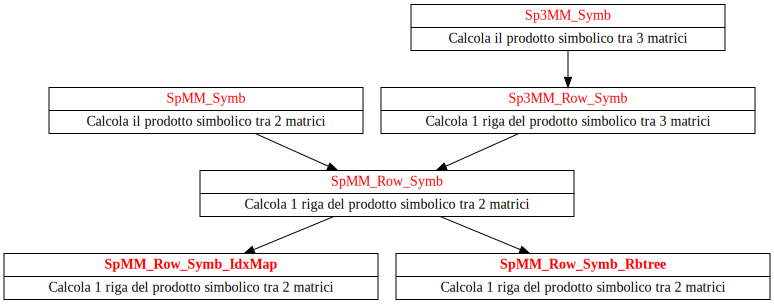
\includegraphics[width=\linewidth,keepaspectratio]{symbProductFunctionDiagram.dot.svg.png} \decoRule
  \label{figCode:symbProductFunctionDiagram}
\end{figure}
\label{SpMM_Row_Symb_}
È possibile notare come la funzione per determinare una riga del prodotto simbolico tra 2 matrici,
\verb|SpMM_Row_Symb_|, sia alla base di tutte le altre.\\ %TODO TRIVIAL?

\subsubsection{Generazione efficiente di versioni differenti di ogni implementazione}
%per Massimizzazione del riuso del codice e dell'efficienza} %TODO better title end?
Il prodotto numerico necessità dei diversi livelli di informazione sulla matrice risultante 
introdotti precedentemente (\ref{chSpMMSymb:outputDetailLevel}
per poter essere implementato con determinati approcci, come verrà descritto nel dettaglio in \ref{chSpMMNum:funcsMultiImplePurpose}.\\

Al fine di massimizzare l'efficienza delle implementazioni e il riuso del codice scritto per generare i vari livelli di output necessari
ho esteso il meccanismo che ho realizzato originariamente per supportare l'integrazione il mio lavoro in un progetto fortran, 
per ottenere varie versioni di ogni funzione relativa al prodotto simbolico.

Mediante un approccio basato su direttive del pre-processore C e molteplici \verb|#include| dei file sorgenti cite{cpp11.2},
sono riuscito ad ottenere automaticamente da una singola funzione sorgente scritta molteplici versioni della stessa,
dove viene modificata la segnatura sorgente nel suffisso del nome e nei parametri.
I dettagli a riguardo di questa tecnica saranno analizzati in \ref{chSpMMAux:multiImplMany}.\\
\label{chSpMMSymb:outputDetailLevel_coreFuncsVersions}
Di seguito le principali versioni alternative delle funzioni per eseguire la fase simbolica di SpMM e Sp3MM.\\
\begin{itemize}
	\item	\verb|OutIdxs_|:
	verranno ritornati, oltre che il \nnnz di ogni (partizione di) riga della matrice risultante,
	anche i relativi indici degli elementi non zero. %della matrice risultante
	\\ \\
	Queste versioni sono necessaria per calcolare il triplo prodotto simbolico,
	come verrà descritto in \ref{chSpMMSymb:Sp3MMSymb}.\\
	Inoltre, sono utili anche ad ottenere direttamente gli indici 
	degli elementi \nnz della matrice risultante (di cui i valori effettivi corrispondenti verranno computati nella fase numerica).\\

	\item	\verb|ColParts_|
	verranno ritornati, oltre che il \nnnz di ogni riga della matrice risultante,
	anche la loro distribuzione per ogni partizione di colonne di ogni riga. %della matrice risultante,
	\\ \\ 
	Queste versioni sono necessaria per eseguire SpMM con un partizionamento bidimensionale dei dati
	come verrà descritto in \ref{chSpMMNum:parti2D}.\\

\end{itemize}

% TODO TODO branch predictors (su path perfettamente predicibile \forall thread) + OutOfOrder exe possono rendere overhead di implementazione 
% TODO TODO con flag per livello dettaglio output e serie di if espliciti sostanzialmente con stesse performance di versione con multiple implementazioni
% TODO TODO tuttavia l'assenza di quei branch nei sorgenti può portare a maggiori ottimizzazioni in compilazione. uncomment ready ;)
%%\subsubsection{Confronto con un semplice approccio funzionale}

\label{chSpMMSymb:funcsMultiImpleVSmanualMultiFunc}
%%Nel caso di implementare la funzione \verb|SpMM_Row_Symb_|, alla base del Prodotto Simbolico accurato \ref{chSpMMSymb:accurateBaseBlock},
%%è possibile paragonare questa metodologia implementativa ad un approccio funzionale in cui le varie versioni 
%%necessarie sono implementate in una funzione singola, componendo sotto funzioni ausiliarie e blocchi di codice su necessità con l'ausilio di \vvv{if}.
%%La speculatività dei processori moderni mediante branch predictor e esecuzione OutOfOrder può portare questa soluzione alternativa ad avere
%%potenzialmente a performance simili rispetto a quelle ottenibili da un codice in cui le istruzioni di branch sono assenti.
%%Tuttavia, la mia soluzione basata su implementazioni multiple, produrra un codice con meno branch, e di conseguenza più ottimizzabile in compilazione.\\

Quest approccio implementativo può portare a diversi benefici, come:
\begin{itemize}
	\item In casi in cui si debba traversare una struttura di indici di supporto
		  è possibile,  con una singola passata, 
		  sia copiare gli indici che tenerne traccia della loro distribuzione in partizioni separate 

	\item Considerando un'altra soluzione, basata su una singola funzione che realizza le varie  %TODO remove?
		  funzionalità richieste per il tipo di output necessario mediante delle condizioni su dei flag come approccio implementativo alternativo.\\
		  Il codice prodotto dal mio approccio implementativo, in seguito alla fase di pre processamento, gode di:
	\begin{itemize}
		\item assenza di tutte le extra istruzioni di branch richieste dall'approccio alternativo. 
			  In questo modo è potenzialmente più ottimizzabile in fase di compilazione.
			  %Tuttavia, escludendo queste ottimizzazione di compilazione, a livello teorico 
			  %la speculatività dei processori moderni mediante branch predictor e OutOfOrder execution, può portare a performance simili
		\item l'uso di meno argomenti per chiamare alcune versioni generate 
			  %% TODO TODO TODO TODO ?? ,che per molte architteture si traduce in meno passaggio dati tra memoria e registri.\\
		\item l'esclusione completa delle istruzioni non necessarie ad ogni versione generata.
	\end{itemize}
\end{itemize}
%symb phase generic description via idx keeper ... row by row based\\
Il Prodotto Simbolico accurato tra 2 matrici $C=A*B$ è realizzato seguendo l'approccio \rowbyrow già descritto: 
mantenendo il conto, senza ripetizioni, degli indici di colonna degli elementi \nnz delle righe di B relativi agli indici di colonna di una riga di A.\\
\label{chSpMMSymb:SpMM_Row_Symb_targetBaseFunc}
Di seguito la realizzazione specifica delle varie versioni della calcolo di una riga del prodotto simbolico
,la funzione \verb|SpMM_Row_Symb_| vista precedentemnte in \ref{SpMM_Row_Symb_},
in base alla struttura di supporto usata per mantenere gli indici degli elementi non zero. 
%la determinazione degli indici degli elementi \nnz di una riga di C (funzione alla base della realizzazione parallela del Prodotto Simbolico, \ref{chSpMMSymb:accurateBaseBlock})

\subsection{Uso di RedBlack tree} \label{chSpMMSymb:usoRBTree}
Usare in parallelo una implementazione di PriorityQueue è un approccio comune
per gestire il mantenimento degli indici \nnz per il Prodotto Simbolico, come fatto da \cite{SpMM_KNL_Multicore_symbsSols}.\\
%Dato il pattern di accesso write-mostly %TODO better CHECKKKK ANd explain
%della fase simbolica dell'operazione di SpMM ho deciso di utilizzare dei RedBlack tree piuttosto che degl'alberi AVL.\\
Tra le varie possibilità disponibili, ho scelto di usare una implementazione di RedBlack tree.\\
L'implementazione dei RedBlack l'ho ricavata personalmente dalla implementazione disponibile nel kernel Linux 5.10.85 (LTS),
mediante un processo di porting in user-space.\\
Il porting in userspace che ho realizzato dei RedBlack tree di linux è disponibile nella mia pagina: \url{https://github.com/andreadiiorio/redblackTree_linux_userspace}.
Dettagli specifici dell'implementazione dei RedBlack tree e del loro processo di adattamento saranno trattati successivamente in \ref{chSpMMAux:linuxRBTree}.\\
%Implementazioni con RBtree 

%operativamente uso:
Per realizzare la funzione target \verb|SpMM_Row_Symb_| con i RedBlack tree in parallelo ho assegnato al thread in esecuzione: 
1 riga di A (corrispondente alla riga target di C) ed 
un RedBlack tree allocato con un numero di nodi sufficiente per la riga più lunga di C.
La riga più lunga della matrice risultante, necessaria per l'implementazione parallela target
è determinata con una riduzione sul risultato di un UpperBound  del prodotto simbolico (visto in \ref{chSpMMSymb:UpperBound}),
con livello informativo dell'output 1 (rispetto alla numerazione introdotta in \ref{chSpMMSymb:outputDetailLevel}).\\
Durante la scansione degli indici $i$ degli elementi \nnz di B, corrispondenti agli elementi \nnz di una riga di A, 
viene effettuato un inserimento di un nuovo nodo con chiave $i$ nel RedBlack tree, se tale chiave non è stata già inserita.
Ogni inserimento avvenuto incrementa il contatore degli elementi \nnz della riga target di C.\\
Per implementare le versioni della funzione target che ritornino anche 
gli indici \nnz effettivi della riga di C (\verb|OutIdxs_|) e la loro distribuzione in partizioni di colonne (\verb|ColParts_|) è sufficiente effettuare 
una singola scansione ordinata delle chiavi $k$ inserite nel RedBlack tree prodotto, andando a salvare $k$ e/o incrementare un contatore
relativo alla partizione di colonne contente $k$.\\
%altro remark di vantaggio = singola passata di rbtree dato l'approccio multi implementazione con cpp
Come già detto la scansione è singola e senza branch relativi a quale versione di \verb|SpMM_Row_Symb_| si sta eseguendo grazie all'approccio
di generazione automatica di diverse implementazioni mediante pre processore.\\
\label{OUT_IDXS_RBTREE_NODES}
Nel caso di eseguire una versione della funzione in oggetto
 che ritorni gli indici degli elementi \nnz della riga risultante, %con \verb|OutIdxs_| nel suffisso del nome,
 il salvataggio della chiave $k$ del RedBlack tree generato,
può avvenire in un array di supporto, allocato precedentemente alla funzione, o 
in alternativa può essere ordinato l'array di nodi RedBlack tree dato in input, \emph{inplace}, 
contenente gli indici degli elementi \nnz della riga target di C come chiavi.\\
%example: building block func signature.
\begin{lstlisting}
static inline idx_t CAT4(SpMM_Row_Symb_Rbtree,OUT_IDXS,COL_PARTS,OFF_F)
  (
   idx_t* aRowJA, idx_t aRowLen, spmat* b,rbRoot* root, rbNode* nodes
   #if _OUT_IDXS  == TRUE && !defined OUT_IDXS_RBTREE_NODES 
   ,idx_t* outIdxs
   #endif
   #if _COL_PARTS == TRUE
   ,ushort gridCols,idx_t* rowColPartsLens
   #endif
  )
\end{lstlisting}
Nel frammento di codice precedente è possibile vedere come la segnatura della funzione in analisi vari in base alla versione da realizzare.
In particolare, il salvataggio degli indici \nnz degli elementi della riga target di C (versione \verb|OutIdxs_|), avviene sull'array di supporto 
\verb|outIdxs| a meno che sia definita la macro di configurazione \verb|OUT_IDXS_RBTREE_NODES|, che comporterà il riordinamento inplace del vettore di 
nodi RedBlack tree \vvv{nodes}, contente gli indici target come chiavi.\\


\subsection{Uso di bitmap di indici o array di flag} \label{chSpMMSymb:structFlagSet}
Usare una struttura contente un insieme di flag per indicare l'appartenenza di indici è un approccio alternativo ai RedBlack
per realizzare la funzione target \verb|SpMM_Row_Symb_| descritta in \ref{chSpMMSymb:SpMM_Row_Symb_targetBaseFunc}, 
potenzialmente con dei benefici prestazionali per alcune versioni.\\
Analogamente al caso dei RedBlack tree, viene assegnato al thread in esecuzione 
1 riga di A, corrispondente alla riga target di C e 
un set di flag, inizializzati a false, di dimensione pari al numero di colonne $N$ di C,
sufficiente a contenere entries per ogni possibile indice della riga target di C.\\
Durante la scansione degli indici di colonna $i$ degli elementi \nnz di B, corrispondenti a una riga di A, 
viene posto a true l'i-esimo flag e, se non era precedentemente posto false, viene anche incrementato il 
contatore degli elementi \nnz della riga target di C.\\
%macro config per scegliere struttura per set di flag
La struttura contenete il set di flag relativi agli elementi \nnz di una riga di C 
è definita nel tipo \verb|nnz_idxs_flags_t| ed è 
configurabile a tempo di compilazione mediante la macro di configurazione \verb|SPVECT_IDX_BITWISE|.
\subsubsection{bitmap di indici}		\label{chSpMMSymb:bitmapsUse}
Se la macro di configurazione \verb|SPVECT_IDX_BITWISE| è settata a \vvv{TRUE}, l'approccio usato sarà quello 
di salvare ogni indice di elementi \nnz all'interno di un insieme di bitmaps.\\
Ogni indice da inserire sarà mappato in un bit specifico, da asserire ad 1, all'interno di una delle variabili del set di bitmaps.
%bitmap sizeing
Nel caso peggiore il set di indici da inserire varia in $(0,N)$, dove $N$ può essere molto grande.\\ 
Usando varibili di dimensione $b$ bits è necessario allocarne al più $\left\lceil \frac{N}{b}  \right\rceil$
per essere in grado di poter mappare l'intero set di indici.\\

Questo approccio è usato sia nel Prodotto Simbolico che Numerico e dettagli ulteriori sull'inserimento e controllo 
di indici nelle bitmaps saranno analizzati in \ref{chSpMMAux:bitmapInsert}.\\
Nel caso di dover realizzare efficientemente la versione \verb|OutIdxs_| ( descritta in \ref{chSpMMNum:funcsMultiImplePurpose} )
della funzione target, è necessario utilizzare una struttura di supporto per salvare tutti gli indici degli elementi \nnz
 che sono stati effettivamente inseriti in una bitmap.
Per per ottemperare a questa necessità ho implementato 2 soluzioni, selezionabili a tempo di compilazione con
la macro di configurazione \verb|IDX_RMUL_SYMB_RBTREE|.\\
\begin{itemize}
	\item se \verb|IDX_RMUL_SYMB_RBTREE| è configurata a \vvv{TRUE}, tutti gli indici da salvare saranno 
		  inseriti in un RedBlack tree, per poi essere successivamente salvati ordinatamente nel array, pre allocato, 
		  da ritornare.
	\item se \verb|IDX_RMUL_SYMB_RBTREE| è configurata a \vvv{FALSE}, tutti gli indici da salvare saranno inseriti
		  (in ordine casuale dipendente dai non zeri delle matrici considerate) direttamente nell'array da ritornare
		  per poi essere ordinati.
\end{itemize}
Entrambi questi approcci hanno un costo computazionale pari a $O(n log n)$ dove n è il numero di indici inseriti.\\

\subsubsection{array di flag}
Alternativamente, se la macro di configurazione \verb|SPVECT_IDX_BITWISE| è settata a FALSE, 
ho realizzato anche un più semplice approccio basato su un array di $N$ $char$, 
dove l'indice di colonna da inserire $i$ corrisponde all $i$-esimo elemento dell'array che avrà valore non zero.\\
La gestione della versione \verb|OutIdxs_| della funzione target è analoga al caso precedente.\\  %trivial?

\subsection{Sp3MM: Calcolo simbolico diretto del triplo prodotto} \label{chSpMMSymb:Sp3MMSymb}
Dato che il problema orinario da risolvere è il triplo prodotto tra matrici sparse per applicazioni come 
amg4psblas \cite{AMG4PSBLAS}, ho deciso di cercare di supportare anche la moltiplicazione diretta 
tra 3 matrici sparse, con un'estensione della formulazione \rowbyrow.\\
Seguendo la notazione introdotta inizialmente in \ref{notazione}, l'approccio seguito è derivato da quello seguito da \cite{Sp3MM4AMG}.\\
Una volta computata la riga $\left(R\cdot AC_i\right)_{r*}$ con la versione \verb|OutIdxs_| di \verb|SpMM_Row_Symb_|, 
questa viene riutilizzata direttamente e con lo stesso approccio \rowbyrow,
per computare la riga relativa della matrice risultante ${AC_{i+1}}_{r*}$.\\ 
Le versioni \verb|OutIdxs_| sono necessarie per ottenere  gli indici di colonne della riga $\left(R\cdot AC_i\right)_{r*}$,
indispensabili per reiterare la formulazione \rowbyrow sulla matrice $P$.\\
L'operazione appena descritta è eseguita in parallelo per ogni riga di $AC_{i+1}$.\\
%Determinare la quantità di elementi \nnz è possibile incontrare durante i primi prodotti tra le righe di $R$ e $AC_i$ è necessario 

\subsection{Pro e contro UpperBound o Prodotto simbolica Accurato} \label{chSpMMSymb:UB_VS_SYMBACC}
La analisi delle differenze prestazionali di implementazioni di SpMM con fase Simbolica Accurata o UpperBound
sarà analizzata in seguito nel capitolo dedicato all'analisi delle performance \ref{ChPerf}.\\
Di seguto qualche considerazione di carattere generale che è possibile trarre dall'analisi di questi approcci differenti.\\
\begin{enumerate}
	\item L'UpperBound gode sicuramente di un costo computazione nettamente inferiore 
	      rispetto a qualsiasi implementazione di Prodotto Simbolico accurato.\\
	\item Tuttavia, questo vantaggio iniziale per soluzioni basate su UpperBound, 
		  è associato alla necessità di dover salvare tutti i risultati intermedi in una struttura temporanea,
		  di cui è necessario effettuare una copia nella matrice risultante.
	\begin{enumerate}
		\item Viceversa il Prodotto Simbolico accurato permette di poter salvare tutti i risultati intermedi,
			  ottenuti durante la fase Numerica, direttamente nella matrice risultante.
	\end{enumerate}
	\item Il Prodotto Simbolico  accurato di $A \cdot B$, 
		  basato su una formulazione derivata da gustavson \cite{gustavson}, ad esempio \rowbyrow,
		  soffre di un ulteriore svantaggio dovuto a dover accedere le righe $B$ in un ordine casuale, derivato 
		  dagli indici degli elementi \nnz della riga corrispondente di A.\\
		  Questo causa potenzialmente un cattivo uso della memoria, come analizzato da 
		  \cite{Sp3MM_for_AMG} ed indirettamente da \cite{ESC}.
	\begin{enumerate}
		\label{chSpMMSymb:UB_VS_SYMBACC_rowbyrowContiguousCopyBack}
		\item Viceversa, il costo addizionale legato allo svantaggio dell'uso di UpperBound menzionato al punto 2,
			  nel caso di una formulazione derivata da gustavson, comporta la copia di risultati intermedi 
			  nella matrice risultante in maniera contigua, come osservato da \cite{Sp3MM_for_AMG}
	\end{enumerate}
	\item In generale, l'overhead di memoria causato dall'UpperBound, potrebbe essere tale da rendere impossibile 
		  sfruttare su GPU una fase simbolica basata su UpperBound. %come osservato da \cite{TODO ritrovalo}
\end{enumerate}
		%tecq symb product
\chapter{Implementazioni OpenMp: Prodotto Numerico}
\label{Chapter3}
%%%% 	ORGANIZZAZIONE
%{Accumulatore denso per i prodotti intermedi}	% breve remark da ch1, flags set per gestione inserimenti idx dups free, snippet di versione con partizionamento
%	{Trasformazione da un accumulatore denso in un vettore sparso}  % brevemenete approccio x passare (efficientemente) da formato denso a sparso
%		XXXX {Allocazione vettori sparsi intermedi} <-> integrare in:	Assegnamento dinamico di spazio per \nnz intermedi ai thread
%{Implementazioni con fase simbolica determinata con UpperBound}	giusto intro?
%   {Assegnamento dinamico di spazio per \nnz intermedi ai thread}  *alloc like atom x assegnare spazio pre allocato ai thread
%   {Assegnamento statico  di spazio per \nnz intermedi ai thread}	approccio con pre divisione (leggero overhead)
									%TODO CONFRONTO TRA I 2 -> teoricamente eguali (meno leggero overhead 2nd) a patto di dare ad ogni thread abbastanza spazio contiguo da fillare (false cache sharing)
%   {Consolidamento risultati intermedi nel risultato finale}	% mergeRows brevemente
%{Implementazioni con fase simbolica accurata} % remark sparisify diretto, implementato con funzione alla base del caso sparsify x versione UpperBound

	%dell'effettivo menziona il come è fatto con snippet semplificato
%{SpMM: Partizionamento monodimensionale}
%{SpMM: Partizionamento bidimensionale}

%{Sp3MM: Calcolo numerico diretto del triplo prodotto tra matrici}, remark approccio rowbyrowbyrow, ...?, snippet

%%%%

%----------------------------------------------------------------------------------------

Prendendo spunto dalle caratteristiche principali degli algoritmi descritti precedentemente in \ref{ChExistingTecqs}, 
in questa sezione vengono descritte implementazioni parallele derivate da gustavson \cite{gustavson} 
con formulazione row-by-row \ref{ChExistingTecqs:formulazioni} per il prodotto numerico tra matrici sparse con OpenMP, 
utilizzando diverse metodologie.
Estendendo l'approccio \rowbyrow, ho realizzato anche una versione per computare un triplo prodotto numerico direttamente.\\
%summing, organizzazione capitolo
In questo capitolo ho organizzato i contenuti per trattare prima dei componenti di supporto e configurazioni del prodotto numerico,
tra cui la differente gestione della memoria in base a quale tipo di prodotto simbolico si sta usando \ref{chSpMMSymb:UpperBound}.\\


\section{Accumulatore denso per le moltiplicazioni scalari intermedie} \label{chSpMMNum:scSparseVectMulPart}
%spiegazione dell'uso acc denso
Come precedentemente visto, una formulazione \rowbyrow di SpMM prevede di computare una riga di $C$ 
mediante la somma di moltiplicazioni scalari intermedie.\\
Analizzando gli ottimi risultati ottenuti da \cite{intelSpMMDenseAccumulator} precedentemente in 
\ref{ssec:intelSpMMDenseAccumulator}, ho deciso di sfruttare l'idea di utilizzare un accumulatore denso per 
sommare le moltiplicazioni scalari intermedie.\\
%double insert by intel paper...
Riguardo la determinazione degli indici di colonna degli elementi \nnz calcolati mediante l'accumulatore denso,
l'articolo menzionato \cite{intelSpMMDenseAccumulator} non specifica l'approccio usato nel dettaglio, 
ma solo che è possibile mantenere efficientemente gli indici inserendoli in un array quando l'elemento relativo nell'accumulatore denso era zero.\\
Tuttavia, quest'approccio è potenzialmente soggetto a reinserimenti di stessi indici in scenari in cui:
i valori \nnz della riga in uso di A comportano un particolare sequenziamento nelle somme delle moltiplicazioni scalari che portano
in una determinata entry dell'accumulatore denso a passare da zero a una serie di valori che 
passano nuovamente per zero (numerico). Date che la entry è tornata a zero, sommandoci un qualsiasi altro valore \nnz 
comporterà di dover reinserire il corrispondente indice.\\
%need my approch
Per quanto questo scenario è discretamente improbabile, %dato che lo zero numerico si ...
nel gestirlo si richiede di dover eliminare gli indici duplicati.\\
Al fine di evitare questa necessità, che potenzialmente richiede una ulteriore passata su tutti gli indici inseriti,
ho deciso di riutilizzare l'idea del set di flag usata per il prodotto simbolico in \ref{chSpMMSymb:structFlagSet}.\\
Ogni indice di colonna di elemento \nnz considerato durante la moltiplicazione scalare richiesta dalla formulazione \rowbyrow, 
verrà inserito in maniera del tutto analoga al caso del prodotto simbolico, incrementando un contatore se l'indice 
non era gia nella struttura ausiliaria di ricerca.\\
Le implementazioni delle bitmap per gestire set di flag saranno descritte in \ref{chSpMMAux:bitmapInsert}.\\
%TODO deconfusiona: reamrk o + ref a fatto che scSparseMul = moltiplicazione scalare è il 1° base step di \rowbyrow 
\begin{lstlisting}
typedef struct{
    double*  v;                     //nnz dense accumulator		(sparsellly filled)
    idx_t*   nnzIdx;                //v's nnz value's indexes		(contiguosily filled)
    idx_t    vLen;
    SPVECT_IDX_DENSE_MAP nnzIdxMap; //nnzIdx's indexed inserted flag set struct
} ACC_DENSE;
\end{lstlisting}
Nel frammento di codice precedente è riportata la struttura utilizzata come accumulatore denso per una riga della matrice risultante $C$.\\
In \vvv{v} saranno accumulati i valori \nnz relativi ad  ed i corrispondenti indici di colonna 
saranno copiati consecutivamente in \vvv{nnzIdx} e settati a \vvv{true} in \vvv{nnzIdxMap}.

\subsection{Trasformazione dell'accumulatore denso in un vettore sparso}	\label{chSpMMNum:sparsify}
L'accumulatore denso calcolato precedentemente deve essere trasformato in un formato sparso per poter essere 
inserito nella matrice target.\\
Per fare questa operazione di \emph{sparsificazione} efficientemente viene utilizzato il vettore degli indici di \vvv{nnzIdx},
come mezzo per accedere solamente alle locazioni dell'accumulatore denso \vvv{v} di interesse,
%Gli indici in \vvv{nnzIdx} si possono accedere direttamente con una \vvv{memcpy}.
%I relativi valori numerici in \vvv{v} devono essere acceduti in un ciclo scansionando gli indici in \vvv{nnzIdx},
come effettuato nel ciclo a riga 4 della seguente funzione.\\
\begin{lstlisting}
static inline void _sparsifyUB(ACC_DENSE* accV,SPACC* accSparse,idx_t startColAcc){
    idx_t nnz = accV->nnzIdxMap.len;
    sort_idx_t(accV->nnzIdx,nnz); //sort nnz idx for ordered write
    for (idx_t i=0,j;    i < nnz;   i++){
        j =  accV->nnzIdx[i];
        accSparse -> JA[i] = j + startColAcc;
        accSparse -> AS[i] = accV->v[j];
    }
    accSparse -> len = nnz;
}
\end{lstlisting}
Nel frammento di codice precedente è possibile notare anche come sia gestita 
la possibilità di convertire un accumulatore denso relativo ad una partizione di riga della matrice risultante, 
gestendo un shifting degli indici di colonna \nnz relativi mediante la variabile \vvv{startColAcc} a riga 6
(necessario per partizionamenti bidimensionali del lavoro come verrà approfondito in \ref{chSpMMNum:parti2D} ).\\
%sort need
Ordinando \vvv{nnzIdx} prima della sua copia nella struttura di destinazione, 
serve a produrre una matrice sparsa in output con indici degli elementi \nnz ordinati.
La necessità di tale operazione dipende dall'uso della matrice successivo al prodotto 
e nel caso CSR la distizione tra formato ordinato e non è riportata da \cite{adaptiveTilingSpMM}.\\
\begin{figure}[h!]
  \centering 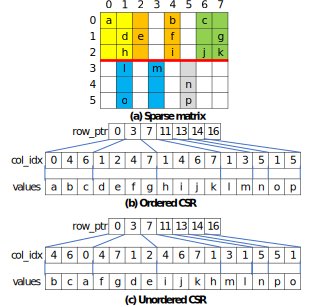
\includegraphics{csrOrderedAndUnordered.svg.png}
  \caption[Distinzione tra matrici CSR con indici di colonna in \vvv{JA} (non) ordinati]
  \decoRule \label{fig:layeredGraphInnerProduct}
\end{figure}
Il costo dell'ordinamento degli indici della matrice risultante è ammortizzato su ogni partizione di riga assegnata ad ogni thread.\\
Ho deciso di implementare l'ordinamento mediante l'implementazione di quicksort
presente nella \vvv{glibc} mediante la funzione \vvv{qsort}.\\


\section{Gestione della memoria in base al tipo di Prodotto Simbolico usato}
Come precedentemente detto in \ref{ChExistingTecqs:openMP_for_philosophy},
è sempre preferibile utilizzare pre allocazioni in luogo di allocazioni dinamiche 
in implementazioni parallele.\\
In base al tipo di fase simbolica effettuata, possono esserci diverse possibilità per 
pre-allocare la memoria per l'operazione di SpMM e successivamente assegnarne 
porzioni ai vari threads.\\
\subsection{Possibilità offerte al Prodotto Numerico, in base al livello di output del Prodotto Simbolico}
\label{chSpMMNum:funcsMultiImplePurpose}
I livelli di output del prodotto simbolico definiti in \ref{chSpMMSymb:outputDetailLevel}, 
permettono di effettuare il prodotto numerico con vari livello di 
partizionamento del lavoro e di uso della memoria:
\begin{itemize}
	\item un prodotto simbolico con output di livello 1 è sufficente a realizzare 
		  il prodotto numerico unicamente salvando i risultati intermedi in una struttura temporanea preallocata,
		  di cui porzioni vengono assegnate ai thread dinamicamente.
		  Dettagli di questo approccio saranno trattati a breve in \ref{chSpMMNum:mallocReplaceAssigns}
	\item un prodotto simbolico con output di livello 2 consente di effettuare il prodotto numerico
		  con partizionamento monodimensionale del lavoro, dove le righe della matrice risultante 
		  possono essere salvate in una struttura temporanea preallocata, di cui porzioni vengono assegnate 
		  staticamente ai thread o direttamente nella matrice risultante nel caso di prodotto simbolico accurato.
	\item un prodotto simbolico con output di livello 3 consente anche di effettuare il prodotto numerico
		  con un partizionamento bidimensionale del lavoro, dove similmente al punto precedente è possibile
		  scrivere le partizioni delle righe della matrice risultante direttamente 
		  in una struttura temporanea o nella matrice risultante se il prodotto simbolico è accurato.
\end{itemize}

\subsection{Uso di una fase simbolica determinata con UpperBound}
Nel caso di utilizzare una fase simbolica rapida basata su UpperBound in una implementazione parallela di SpMM
, come già menzionato in \ref{chSpMMSymb:UB_VS_SYMBACC},
è necessario utilizzare durante la fase numerica una struttura temporanea per salvare i risultati dei prodotti.\\
\label{chSpMMNum:UB_necessitaCopyBack}
Questa necessità è dovuta al fatto che ogni thread non ha informazione sulla esatta dimensione della porzione di
matrice da calcolare e quindi non può scrivere i suoi risultati direttamente nell'output dell'operazione di SpMM.\\
La struttura intermedia che ho utilizzato è composta da una coppia di aree di memoria
dimensionate con l'output della fase simbolica usata, destinate rispettivamente ai
valori dei \nnz e i relativi indici di colonna calcolati durante le moltiplicazioni scalari della fase numerica.\\
Nel seguito verranno indicate le aree per i \nnz e i relativi indici del risultato di SpMM rispettivamente come 
\emph{AS\_tmp JA\_tmp}.\\
\label{chSpMMNum:SPACC}	%keep track UB sparsified starts->lens for rowsMerge
Le partizioni di righe della matrice risultante calcolate verranno scritte da ogni thread
in aree contigue di questa struttura intermedia, salvandone gli indirizzi iniziali 
in questa struttura di supporto.\\
Per supportare l'operazione conclusiva di copia dei risultati intermedi nella matrice output all'operazione di SpMM 
(descritta in \ref{chSpMMNum:mergeRows}) viene utilizzata la seguente struttura:
\begin{lstlisting}
//Sparse vector accumulator
typedef struct{                                               
    double* AS;    //row part nnz values                                         
    idx_t*  JA;    //row part nnz indexes
    idx_t   len;   //rowLen
} SPACC;           
\end{lstlisting}
Nella struttura precedente, con una notazione CSR, si rappresenta un generico vettore sparso 
con \vvv{len} elementi \nnz in \vvv{AS} e relativi indici (di colonna nela caso CSR) in \vvv{JA}.
Il thread che avrà determinato una partizione di una riga della matrice target
scriverà i valori \nnz e i relativi indici in 2 blocchi di memoria della struttura temporanea,
annotandone i rispettivi indirizzi inziali nei puntatori \vvv{AS JA} e la lunghezza in \vvv{len}.\\
%dyn or static assign blocks
L'assegnazione delle aree di memoria della struttura intermedia per i risultati computati 
da ogni thread è gestita in modo dinamico o statico.
È possibile selezionare quest'ultimo approccio a tempo di compilazione in luogo dell'altro
definendo la macro \verb|SPARSIFY_PRE_PARTITIONING| con valore {TRUE}.\\

\subsubsection{Assegnamento dinamico di spazio per non zeri intermedi ai thread} \label{chSpMMNum:mallocReplaceAssigns}
Un approccio di assegnazione di porzioni di \emph{AS\_tmp JA\_tmp} simile ad effettuare allocazioni 
dinamiche, ma senza le criticità di performance citate in \ref{ChExistingTecqs:openMP_for_philosophy}
è il seguente.\\
\label{chSpMMNum:sparsifyMallocReplace}
Ogni thread che necessita di \emph{sparsificare} l'accumulatore denso determinato durante 
le moltiplicazioni scalari in un'area di memoria può incrementare {\bf{atomicamente}} un 
indice relativo alla fine dell'ultima area di memoria assegnata ad un qualsiasi altro thread,
catturandone il valore precedente.\\
\label{chSpMMNum:sparsifyMallocReplace_EASY_INTEGRATION_IN_EVERY_UB_PARTITIONING}
Questa soluzione di gestione dello spazio intermedio ha il vantaggio di richiedere quasi
nessuna informazione dal prodotto simbolico (è sufficiente un output di livello 1 secondo la numerazione descritta in \ref{chSpMMSymb:outputDetailLevel})
indipendentemente dal particolare tipo di partizionamento del lavoro che si sta utilizzando.\\
%code 
Segue la funzione per trasformare l'accumulatore denso in formato sparso con questo approccio.\\
\begin{lstlisting}
//row[Part] sparsified in a thread safe reserved area using atomics
static inline void sparsifyUBNoPartsBounds
  (SPMM_ACC* acc,ACC_DENSE* accV,SPACC* accSparse, ulong startColAcc){
    idx_t nnz = accV->nnzIdxMap.len;
    idx_t sparsifyStartV;
    sparsifyStartV = __atomic_fetch_add(&(acc->lastAssigned),nnz,__ATOMIC_ACQ_REL); 
    accSparse -> AS = acc->AS + sparsifyStartV;
    accSparse -> JA = acc->JA + sparsifyStartV;
    _sparsifyUB(accV,accSparse,startColAcc);
}
\end{lstlisting}
Nel frammento di codice precedente, è possibile vedere come a riga a 6 venga usata
la builtin di gcc \verb|__atomic_fetch_add| \cite{gcc10.1}
per riservare al thread corrente una porzione di memoria di \emph{AS\_tmp JA\_tmp}
a riga 7 e 8, per scrivere i risultati intermedi computati.\\
La primitiva \verb|__atomic_fetch_add| permette di incrementare una locazione 
di memoria, ritornandone il valore non incrementato.
Ulteriori dettagli su questo approccio e su alcune varianti saranno analizzati in \ref{chSpMMAux:atomicSegAssign}

\subsubsection{Assegnamento statico  di spazio per \nnz intermedi ai thread} \label{chSpMMNum:preSplitAS_JA_tmp}
Un'alternativa semplice all'approccio precedente (\ref{chSpMMNum:mallocReplaceAssigns}),
è quello di effettuare una suddivisione per ogni (partizione di) riga della matrice risultante
dello spazio allocato in \emph{AS\_tmp JA\_tmp}, così da consentire ad ogni thread 
di poter scrivere i propri risultati intermedi in una spazio non soggetto a race-conditions.\\
Per realizzare questo è necessario avere conoscenza di un UpperBound per ogni (partizione di)
riga della matrice risultante, e conseguentemente è necessario utilizzare un prodotto simbolico
con un livello di dettaglio dell'output di livello 2 (3), 
seguendo la nomenclatura introdotta nel capitolo precedente \ref{chSpMMSymb:outputDetailLevel}.\\

\subsubsection{Consolidamento risultati intermedi nel risultato finale} \label{chSpMMNum:mergeRows}
In conclusione all'operazione di SpMM con fase simbolica basata su UpperBound, 
è necessario raccogliere tutti i valori \nnz e i relativi indici,
calcolati nella struttura temporanea ( \emph{AS\_tmp JA\_tmp} ) nella matrice risultante di output.
Per fare questo è sufficiente copiare solo gli elementi \nnz scritti nella struttura temporanea
mediante le strutture ausiliare \vvv{SPACC}, descritte in \ref{chSpMMNum:SPACC}.\\
Segue la funzione per radunare tutti i risultati intermedi relativi a partizioni di righe della matrice 
risultante nell'output dell'operazione di SpMM.\\
\begin{lstlisting}
inline int mergeRowsPartitions(SPACC* rowsParts,spmat* mat,CONFIG* conf){
	//offsets for preparing copy 
    idx_t nzNum=0,j,rLen,idx,partsNum = mat->M * conf->gridCols;
    idx_t* rowsPartsOffsets; //partsNum offsets for each row's partitiong of mat
    for (idx_t r=0; r<mat->M; r++){	///count nnz entries offsets per row's part.
        for (j=0,rLen=0; j<conf->gridCols; j++){
            idx = IDX2D(r,j,conf->gridCols);
            rowsPartsOffsets[idx]=nzNum+rLen; //part start=prev accumulated end
            rLen += rowsParts[idx].len;
        }
        nzNum += rLen;
        mat->IRP[r+1] = nzNum;
		#ifdef ROWLENS
        mat->RL[r] = rLen;
		#endif
    }
    mat->NZ = nzNum;
	...
	//copy
    idx_t pLen; //omp for aux vars
    #pragma omp parallel for schedule(static) private(pLen)
    for (idx_t i=0;  i<partsNum; i++){
        pLen = rowsParts[i].len;
        memcpy(mat->AS + rowsPartsOffsets[i],rowsParts[i].AS,pLen*sizeof(*(mat->AS)));
        memcpy(mat->JA + rowsPartsOffsets[i],rowsParts[i].JA,pLen*sizeof(*(mat->JA)));
    }
    return EXIT_SUCCESS;
}
\end{lstlisting}
Come è possibile vedere nel frammento di codiceprecedente, l'operazione di copia dei risultati
intermedi nella matrice risultante è divisa in 2 fasi.\\
Tra riga 5 e 16, viene cumulata la dimensione di tutti i blocchi di \nnz computati
nel prodotto numerico in un vettore ausiliario \vvv{rowsPartsOffsets} e nella componente 
\vvv{IRP} della matrice risultante.\\
Successivamente la copia vera e propria avviene in parallelo 
a livello di singola partizione di riga risultante nel ciclo a riga 22 mediante delle \vvv{memcpy}.\\
Ad ogni iterazione si preleveranno i \nnz scritti nella struttura temporanea realativi
alla partizione $i~mod~ \verb|conf->gridCols|$-esima della $\left\lfloor \frac{i}{\text{conf} \rightarrow \text{gridCols}} \right\rfloor$
riga dalla struttura temporanea, copiandoli nella posizione appropriata della matrice risultante.\\



\subsection{Uso di una fase simbolica accurata}
Nel caso di utilizzare un Prodotto Simbolico accurato, è possibile \emph{sparsificare}
gli accumulatori densi ottenuti sommando le moltiplicazioni scalari \ref{chSpMMNum:scSparseVectMulPart}
direttamente nella matrice risultante.\\
Per fare questo è necessaria una piccola operazione di inizializzazione della matrice di output
andando a popolare il vettore \vvv{IRP}, con la cumulazione del \nnnz delle 
(partizioni di) righe determinato durante la fase simbolica.\\

%%%%%%%%%%%%%%%%%%%%%%%%  CORE NUMERICAL PRODUCT  %%%%%%%%%%%%%%%%%%%%%%%%%%%%%%
\section{Esecuzione del Prodotto Numerico}
In questa sezione verranno analizzate metodologie per effettuare l'operazione di SpMM in parallelo,
considerando vari approcci di suddivisione dei dati tra i thread.\\
%%%% diff _UB_ and _SymbNum_ version
Come già detto l'uso di una fase simbolica accurata o basata su UpperBound, discrimina la necessità 
o meno di dover utilizzare una struttura intermedia durante il prodotto numerico.
Oltre questo dettaglio non ci sono particolari differenze nelle due implementazioni della fase numerica
e per questo si analizzeranno nel seguito le implementazioni che sono supportate da un prodotto simbolico basato su UpperBound.\\
%rewind \rowbyrow + extra description + adattamento per partizionamento 2D
La formulazione \rowbyrow, come indicato in \ref{ChExistingTecqs:formulazioni}, 
calcola la riga $c_{i*}$ della matrice risultante sommando i vettori ottenuti dalle moltiplicazioni scalari tra:
gli elementi $a_{ik} \in a_{i*}$ della corrispondente riga della matrice $A$ e  
le righe di $b_{k*} \in B$ relativi agli indici di colonna $k$ degli elementi $a_{ik}$.
Questa operazione è esprimibile in maniera compatta come:\\
$c_{i*} = \sum\limits_{k \in I_i(A)}  a_{ik} \ast  b_{k*}$.\\
È possibile derivare il calcolo della partizione di colonne $c_z - c_w$ della riga $c_{i*}$
limitando le moltiplicazioni scalari $a_{ik} \ast  b_{k*}$ alle relative partizioni di colonne della matrice $B$. 
L'operazione appena descritta è esprimibile in maniera compatta seguendo la notazione introdotta \ref{notazione} come:\\
$c_{i~c_z-c_w} = \sum\limits_{k \in I_i(A)}  a_{ik} \ast  b_{k~c_z-c_w}$.\\

\subsection{Partizionamento monodimensionale}
Un semplice partizionamento delle matrici per parallelizzare SpMM, è quello di 
assegnare righe intere o blocchi di righe della matrice da calcolare $C$ ai thread.\\
%partitioning terminology
Nella terminologia introdotta precedentemente in \ref{ChExistingTecqs:workCube}, equivale ad
assegnare gruppi di Layers del cubo di lavoro ai vari threads.\\
Segue una parte del codice per effettuare l'operazione di SpMM con 
un partizionamento dei dati di blocchi di righe della matrice A e C:    \label{chSpMMNum:part1DGroup}
\begin{lstlisting}
    #pragma omp parallel for schedule(runtime) private(acc,startRow,block)
    for (b=0;   b < cfg->gridRows; b++){
        block		= UNIF_REMINDER_DISTRI(b,rowBlock,rowBlockRem);
        startRow	= UNIF_REMINDER_DISTRI_STARTIDX(b,rowBlock,rowBlockRem);
        acc			= accVects + omp_get_thread_num();
        for (ulong r=startRow;  r<startRow+block;  r++){
            for (ulong c=A->IRP[r]-OFF_F; c<A->IRP[r+1]-OFF_F; c++) 
                CAT(scSparseRowMul_,OFF_F)(A->AS[c], B, A->JA[c]-OFF_F, acc);
            //trasform accumulated dense vector to a CSR row, in a tmp storage struct
        	#if SPARSIFY_PRE_PARTITIONING == T
			_sparsifyUB(acc,outAccumul->accs+r,0);
			#else
        	sparsifyUBNoPartsBounds(outAccumul,acc,outAccumul->accs + r,0);
			#endif
            _resetAccVect(acc);   //rezero for the next A row
        }
    }
    ///merge sparse row computed before in output matrix
    if (mergeRows(outAccumul->accs,AB))    goto _err;
\end{lstlisting}
Nel frammento di codice precedente è possibile vedere come ogni thread determini 
il proprio blocco di righe su cui operare a riga mediante la macro \verb|UNIF_REMINDER_DISTRI_STARTIDX|,
che consente di determinare blocchi di dimensione il più uniforme possibile  
effettuando una suddivisione del resto della divisione intera tra il numero di righe e \vvv{cfg->gridRows},
ovvero il grado di partizionamento monodimensionale della matrice.
Maggiori dettagli e considerazioni a riguardo di quest'approccio di distribuzione saranno
descritti in \ref{chSpMMAux:UNIF_REMINDER_DISTRI}.\\
Nel ciclo a riga 6, il thread accumulerà le moltiplicazioni scalari nel suo accumulatore denso
determinato a riga 5, per poi \emph{sparsificarne} la riga risultante con
una politica di assegnamento statica o dinamica dello spazio temporaneo pre allocato,
rispettivamente a riga 11 o 13 (come affrontato rispettivamente in 
\ref{chSpMMNum:mallocReplaceAssigns} e \ref{chSpMMNum:preSplitAS_JA_tmp} ).\\
Dopo aver calcolato e \emph{sparsificato}, una riga della matrice risultante, è 
necessario resettare l'accumulatore denso relativo usato (riga 15).\\
Al termine del calcolo di tutte le righe, è necessario raccoglierle dallo spazio temporaneo usato
alla matrice risultante a riga 19 (come visto in \ref{chSpMMNum:mergeRows}).\\

\subsection{Partizionamento bidimensionale} \label{chSpMMNum:parti2D}
Un partizionamento 2D dell'operazione di SpMM è quello di assegnare ai threads 
blocchi bidimensionali della matrice C ottenuti dalla moltiplicazione di
blocchi di righe della matrice A e blocchi di colonne della matrice B.
Questa tecnica è stata rappresentata graficamente in \ref{fig:gustavsonRigheBlocksGraphicalIntel}.\\
%partitioning terminology
Nella terminologia introdotta precedentemente in \ref{ChExistingTecqs:workCube}, equivale ad
assegnare gruppi di fibers del cubo di lavoro ai vari threads.\\
%details now
In questo caso le moltiplicazioni scalari saranno limitate a partizioni di colonne di B,
conseguentemente è possibile utilizzare un accumulatore denso dimensionato sulla più grande
partizione di colonne di B da analizzare.\\
Ho deciso di seguire questo approccio per risparmiare allocazioni temporanee di memoria, 
al costo di dover gestire uno \emph{shifting} degl'indici introdotti nell'accumulatore denso
durante le operazioni di
somma di moltiplicazioni scalari e \emph{sparsificazione} degli accumulatori densi.\\
\label{chSpMMNum:csrColPartitioning}
Al fine di effettuare un partizionamento della matrice CSR B per blocchi di colonne 
ho realizzato due approcci, uno basato su una struttura ausiliaria di offset per accedere le partizioni della matrice originale
ed uno basato sul copiare la matrice in sotto matrici corrispondenti alle partizioni da accedere.
Dettagli sulle tecniche di partizionamento per colonne di una matrice CSR saranno analizzate
separatamente in \ref{chSpMMAux:csrColPartitioning}\\
Dal momento che il codice relativo all'uso di questi due approcci nel Prodotto Numerico è molto simile
segue una descrizione del caso più semplice basato sulla copia delle partizioni di B in sotto matrici.\\

\subsubsection{Partizionamento delle colonne di B in matrici separate}
Segue l'implementazione del Prodotto Numerico con partizionamento bidimensionale del lavoro,
sfruttando il partizionamento delle righe di A descritto in \ref{chSpMMNum:part1DGroup}
e il partizionamento per colonne di B che verrà descritto in \ref{chSpMMAux:csrColPartitioningAllocatd}
\begin{lstlisting}
    #pragma omp parallel for schedule(runtime) private(accV,accRowPart,...)
    for (tileID = 0; tileID < gridSize; tileID++){
        ///get iteration's indexing variables
        //tile index in the 2D grid of AB computation TODO OMP HOW TO PARALLELIZE 2 FOR
        t_i = tileID/cfg->gridCols;  //i-th row block
        t_j = tileID%cfg->gridCols;  //j-th col block
        //get tile row-cols group FAIR sizes
        rowBlock = UNIF_REMINDER_DISTRI(t_i,_rowBlock,_rowBlockRem); 
        startRow = UNIF_REMINDER_DISTRI_STARTIDX(t_i,_rowBlock,_rowBlockRem);
        startCol = UNIF_REMINDER_DISTRI_STARTIDX(t_j,_colBlock,_colBlockRem);
        
        colPart = colPartsB + t_j;
        accV = accVectors + tileID; 
         
        for (ulong r=startRow;  r<startRow+rowBlock;  r++){		///compute (A*B)[:t_i:][:t_j:]
            //iterate over nz col index j inside current row r
            //row-by-row restricted to colsubset of B to get AB[r][:colBlock:]
            for (ulong j=A->IRP[r]-OFF_F,c,bRowStart,bRowLen; j<A->IRP[r+1]-OFF_F; j++){
                //get start of B[A->JA[j]][:colBlock:]
                c = A->JA[j]-OFF_F; // column of nnz entry in A[r][:] <-> target B row
                bRowStart = colPart->IRP[c];
				#ifdef ROWLENS
                bRowLen   = colPart->RL[c];
				#else
                bRowLen   = colPart->IRP[c+1] - bRowStart;
				#endif
                CAT(scSparseVectMulPart_,OFF_F)(A->AS[j],colPart->AS+bRowStart,colPart->JA+bRowStart,
                    bRowLen,startCol,accV);
            }

            accRowPart = outAccumul->accs + IDX2D(r,t_j,cfg->gridCols);
			#if SPARSIFY_PRE_PARTITIONING == T
			_sparsifyUB(accV,accRowPart,startCol);
			#else
            sparsifyUBNoPartsBounds(outAccumul,accV,accRowPart,startCol);
			#endif
            _resetAccVect(accV);
        }
    }
    if (mergeRowsPartitions(outAccumul->accs,AB,cfg))  goto _err;
\end{lstlisting}
Ogni thread è delegato al calcolo di un blocco 2D della matrice C,
identificato dagl'indici \verb|t_i| \verb|t_j|, 
moltiplicando un blocco di righe della matrice A e un blocco di colonne della matrice B,
identificati dalle variabili in righe 8-12.\\
Come nel caso monodimensionale, i blocchi assegnati ai thread sono di dimensione il più possibile uniforme.\\
Nel ciclo a riga 15, il thread corrente computerà la \verb|t_j|-esima partizione della riga \verb|r| di C, 
in un accumulatore denso che verrà \emph{sparsificato} a riga 32-36,
tenendo traccia dell'indice inziale della partizione di B in \vvv{startCol} per gestire lo 
shifting degli indici necessario ad usare un accumulatore denso dimensionato alla 
partizione di riga più grande di B.\\
Infine, a riga 40, tutte le partizioni di righe calcolate verranno unificate dalla struttura 
temporanea \vvv{outAccumul} alla matrice di output \vvv{AB},
in maniera analoga al caso precedente monodimensionale.\\


\subsection{Sp3MM: Calcolo numerico diretto del triplo prodotto tra matrici} \label{chSpMMNum:directProduct}
Dato che il problema orinario da risolvere è il triplo prodotto tra matrici sparse per applicazioni come 
amg4psblas \cite{AMG4PSBLAS\_Git}, ho deciso di di supportare anche 
la fase numerica della moltiplicazione diretta tra 3 matrici sparse, con un estenzione della formulazione \rowbyrow.
%mediante un partizionamento 1D ed una fase simbolica basata su UpperBound.\\ %TODO SOLO EURISTICA FACILE TESTATA.
L'approccio che ho seguito è derivato dal lavoro di \cite{Sp3MM4AMG} 
ed è basato sul riuso diretto delle righe computate con la formulazione \rowbyrow,
per determinare le righe della matrice finale, senza l'ausilio di una matrice contente un'operazione di SpMM intermedia.\\ 
Nel seguito si seguirà la notazione introdota inizialmente riguardo il triplo prodotto tra matrici sparse (\ref{notazioneSp3MM}).\\
%Core summarizing steps for Sp3MM
Il primo passo per l'operazione di Sp3MM è calcolare la riga $\left( R \cdot AC_i \right)_{r*}$ 
sottoforma di accumulatore denso \vvv{accRAC}, sommando i risultati delle moltiplicazioni scalari relative alla formulazione \rowbyrow.\\
Successivamente, indicizzando \vvv{accRAC} esattamente come fatto nella \emph{sparsificazione} di SpMM (\ref{chSpMMNum:sparsify}),
è possibile ottenere la riga della matrice target ${AC_{i+1}}_{r*} = \left(R\cdot AC_i\cdot P\right)_{r*}$ 
reiterando l'operazione di SpMM tra la riga ottenuta sottoforma di accumulatore denso e la matrice $P$.\\
%code
Di seguito il blocco di codice principale per realizzare questa operazione.\\
\begin{lstlisting}
#pragma omp parallel for schedule(runtime) private(accRAC,accRACP,c)
for (ulong r=0;  r<R->M; r++){    //row-by-row-by-row formulation
    accRAC  = accVectorsR_AC  + omp_get_thread_num();
    accRACP = accVectorsRAC_P + omp_get_thread_num();
	//computing (tmp) R*AC r-th row
    for (idx_t j=R->IRP[r]-OFF_F; j<R->IRP[r+1]-OFF_F; j++)
        CAT(scSparseRowMul_,OFF_F)(R->AS[j], AC, R->JA[j]-OFF_F, accRAC);
    //forward the computed tmp row for the final matrix's row
    for (idx_t j=0; j<accRAC->nnzIdxMap.len; j++){
        c = accRAC->nnzIdx[j];    
        CAT(scSparseRowMul_,OFF_F)(accRAC->v[c],P,c,accRACP);
    }
\end{lstlisting}
Come è possibile vedere, la \vvv{r}-esima riga di $R\cdot AC_i$ ottenuta a linea 7 sotoforma di accumulatore denso,
viene immediatamente riusata per determinare la \vvv{r}-esima riga di $AC_{i+1}$ a linea 11,
indicizzandola come fatto dalle funzioni di \emph{sparsificazione} analizzate in precedenza,
nel ciclo a riga 9.\\
			%tecq num  product
\chapter{Componenti di supporto a Sp[3]MM}
In questo capitolo verranno analizzati diversi componenti ausiliari
sviluppati ed integrati per supportare le operazioni di SpMM e Sp3MM.\\
%%%%%%%%%%%%%%%%%%%%%%  CORE  -- >> << -- xD  %%%%%%%%%%%%%%%%%%%%%%%%%%%%%%%%%%
\section[Derivazione di molteplici implementazioni con PreProcessore C]	
{Derivazione automatica di molteplici implementazioni mediante PreProcessore C}	\label{chSpMMAux:multiImpl}
Sfruttando una serie di direttive del pre processore C, sono riuscito ad ottenere
per molte funzioni scritte nei sorgenti, varie versioni differenti ottenute a tempo di pre-processamento, 
accessibili in altre funzioni mediante una segnatura modificata.\\
La necessità principale di realizzare questo approccio è stato quello di supportare, con
un'alta efficienza, l'integrazione del codice C in un progetto fortran come \cite{PSBLAS3},
come verrà trattato a breve in \ref{chSpMMAux:fortranIntegrate}.\\
%PRO GENERAL CPP MULTI VERSION IMPLEMENTATIONS
I vantaggi di usare il pre processore per ottenere molteplici versioni di una funzione sono diverse:
\begin{itemize}
	\item	la possibilità di escludere completamente sezioni di codice non utili ad una versione
	\item	la possibilità di aumentare di molto il riuso del codice scritto
	\item	rispetto ad incapsulare in sotto funzioni le differenze delle varie versioni da ottenere
			rispetto ad una funzione  base:
	\begin{itemize}
		\item	si consente al compilatore di effettuare ottimizzazioni 
				su ogni versione ottenuta in seguito al pre processamento, non possibili a run-time,
				come ad esempio semplificare un offset pari a zero da applicare ad operazioni di indicizzazione
				%(come ad esempio usare una diversa indicizzazione all'interno di un applicazione Fortran
				%\ref{chSpMMAux:fortanIdxsDifferent} )
		\item	evitare istruzioni di branching addizionali nel codice, (come analizzato in \ref{chSpMMSymb:funcsMultiImpleVSmanualMultiFunc} )
				che potenzialmente permettono ulteriori ottimizzazioni a tempo di compilazione.\\
	\end{itemize}
\end{itemize}
Ho pubblicato un semplice esempio di questo approccio implementativo in \url{https://github.com/andreadiiorio/C_Compile_Multi_Implementation_Automatically}.\\
\voidLine
Per ottenere diverse implementazioni da una funzione è necessario:
\begin{itemize}
	\item	racchiudere le differenze richieste da ogni versione in una funzione \emph{base o generica} con una serie di direttive \verb|#if ... #endif| ,\\
			così da consentire al preprocessore l'aggiunta del codice necessario a modificare la funzione base.%ad una particolare versione.
	\item	Le diverse versioni della funzione \emph{generica} devono essere esportate ad altre funzioni mediante una segnatura differente.\\
			Per questo è possibile aggiungere un  suffisso al nome ed eventualmente argomenti addizionali alla funzione 
			\emph{base}, mediante la concatenazione di stringhe del pre-processore C.\\
			Un possibile approccio per supportare la concatenazione di stringhe e macro di configurazione
			in questo contesto è quello di usare la macro \vvv{CAT} del seguente blocco di codice.\\
			\begin{lstlisting}
#define _STR(s) #s
#define STR(s) _STR(s)

//Concatenate preprocessor tokens A and B WITHOUT   expanding macro definitions
#define _CAT(a,b)    a ## b
//Concatenate preprocessor tokens A and B           EXPANDING macro definitions
#define CAT(a,b)    _CAT(a,b)
			\end{lstlisting}
	\item	Le funzioni generiche devono essere racchiuse in un sorgente dedicato, ed incluse da un altro mediante \verb|#include|,
			per un numero di volte pari al numero di versioni che è necessario ottenere,
			ridefininendo le macro ausiliare di configurazione delle implementazioni differenti.
	\item	per avere esportate le dichiarazioni delle versioni differenti realizzate, è possibile reiterare l'approccio 
			appena descrito agli header files.
\end{itemize}
 
\subsection{Supporto integrazione in progetto Fortran} \label{chSpMMAux:fortranIntegrate}
Al giorno d'oggi esistono vari approcci per integrare un applicazione C in una Fortran e viceversa,
grazie agli standard del linguaggio Fortran 2003 e 2018, come descritto in \cite{modernFortranExplained}.\\
Una differenza sostanziale di questi due linguaggi è l'uso di una differente indicizzazione, 
dove il C è a base 0 e il Fortran è a base 1.\\
%need double indexing generic
È necessario tenere a mente questa differenza dato che in ogni formato di memorizzazione sparso di matrici 
sono presenti degli indici relativi alla posizione dei valori \nnz nella matrice.\\
%efficient approch
Per supportare l'integrazione di questo lavoro in \cite{AMG4PSBLAS},
è stato necessario supportare efficientemente un passaggio tra l'indicizzazione
dell'applicazione fortran a quella C per eseguire il prodotto, eseguendo poi il vicerversa 
nel ritorno all'applicazione chiamante.\\
Al fine di supportare efficientemente il cambio di questi indici 
ho sfruttato l'approccio descritto per ottenere 2 versione per ogni funzione,
una che accetti l'indicizzazione nativa del C e un'altra che accetti l'indicizzazione del Fortran,
mediante l'aggiunta di un suffisso numerico ad ogni nome di funzione %.\\
come nell'esempio successivo.\\ 
\begin{lstlisting}
spmat* CAT(spmmRowByRow_SymbNum_,OFF_F)(spmat* A,spmat* B, CONFIG* cfg){...}
\end{lstlisting}
Dalla funzione precedente, definita nel file \verb|Sp3MM_CSR_OMP_Symb_Generic.c| per eseguire il prodotto numerico con un partizionamento del lavoro 1D 
verranno ottenute due versioni distinte per supportare le due indicizzazioni in base al valore della macro \verb|OFF_F| al momento
dell'inclusione del sorgente.\\
La doppia indicizzazione è realizzata dall'uso della macro \verb|OFF_F| all'interno della funzione 
come costante sottratta ad ogni indice preveniente dal Fortran prima di utilizzarlo per indicizzare un qualsiasi vettore,
ed avrà valore \vvv{1} nella versione da usare in un'applicazione Fortran o \vvv{0} per una applicazione C.\\
Un vantaggio immediato di avere una versione dedicata all'indicizzazione C è quello di avere la certezza 
quasi assoluta che la correzione degli indici con il valore \vvv{0} in \verb|OFF_F| verrà ottimizzata via dal compilatore.\\
%defined interface
Inoltre, per favorire una interoperabilità tra le varie implementazioni per le operazioni di SpMM e Sp3MM 
ho definito le seguenti interfacce per le operazioni:
\begin{lstlisting}
typedef spmat* (*SPMM_INTERF )  (spmat*,spmat*,CONFIG*);
typedef spmat* (*SP3MM_INTERF)  (spmat*,spmat*,spmat*,CONFIG*,SPMM_INTERF);
\end{lstlisting}
Dove \vvv{spmat} è una struttura con campi per supportare varie rappresentazioni sparse 
come CSR o ELL, mentre \vvv{CONFIG} contiene la configurazione per le esecuzioni delle operazioni in oggetto,
come ad esempio la griglia di parallelizzazione del lavoro o il numero di thread da utilizzare.\\

Per supportare il lato Fortran dell'integrazione è stato sfruttato il modulo \verb|iso_c_binding| 
per definire le interfacce e strutture con controparte nel codice C, in un modulo di supporto.\\

\subsection{Generazione efficiente di diverse versioni di una funzione base}	\label{chSpMMAux:multiImplMany}
Estendendo la soluzione appena riportata per generare una coppia di implementazioni per gestire una doppia indicizzazione,
ho realizzato un supporto alla generazione di otto versioni differenti di una funzione generica nel modulo relativo al prodotto simbolico.\\
Per realizzare le varie combinazioni di versioni richieste di ogni funzione per generare i vari livelli di dettaglio dell'output 
del prodotto simbolico descritti in \ref{chSpMMSymb:outputDetailLevel_coreFuncsVersions},
ho usato il seguente approccio basato su redefinizioni di alcune macro di supporto:\\
\begin{lstlisting}
#define OFF_F 0
	///generate basic versions
	#include "Sp3MM_CSR_OMP_SymbStep_Generic.c"
	///generate outIdxs versions
	#define OUT_IDXS 	OUT_IDXS_ON	
		#include "Sp3MM_CSR_OMP_SymbStep_Generic.c"
	#undef  OUT_IDXS
	///generate colParts versions
	#define COL_PARTS	COL_PARTS_ON
		#include "Sp3MM_CSR_OMP_SymbStep_Generic.c"
		//generate outIdxs AND colParts versions
		#define OUT_IDXS 	OUT_IDXS_ON
		#include "Sp3MM_CSR_OMP_SymbStep_Generic.c"

	#undef OUT_IDXS
	#undef COL_PARTS
#undef OFF_F
#define OFF_F 1
...
\end{lstlisting}
Nel frammento di codice precedente vengono generate dal preprocessore C otto diverse versioni
della maggior parte delle funzioni definite nel sorgente \\ \verb|Sp3MM_CSR_OMP_SymbStep_Generic.c|
combinando la ridefinizione delle macro di configurazione \verb|OUT_IDXS COL_PARTS OFF_F|.\\

\section{Linux Kernel 5.10.85 RedBlack Tree Userspace porting} \label{chSpMMAux:linuxRBTree}
L'implementazione dei RedBlack Tree usati nel prodotto simbolico è ottenuta effettuando un porting in 
userspace dei moduli relativi del kernel Linux 5.10.85.\\
\subsection{RedBlack nel kernel Linux}
\begin{figure}[H]
  \centering \includegraphics[width=.7\linewidth,keepaspectratio]{Red-black_tree_example.svg.pdf}
  \caption{Rappresentazione grafica di un RedBlack Tree}
  \decoRule \label{fig:rbtree}
\end{figure}
I RedBlack Tree sono delle strutture di ricerca molto efficienti catalogabili come 
\emph{Alberi binari auto bilanciati}.\\%self//semi-balancing binary search tree
La loro formulazione comprende diversi vincoli strutturali, da mantenre in seguito ad ogni operazione di inserimento o cancellazione,
che garantiscono ottime proprietà di bilanciamento tra cui avere che:\\ %| path: root ⟶ foglia più lontana | ≤  2* | path: root ⟶ foglia più vicina |
la distanza tra la radice dell'albero e la foglia più lontana è minore o uguale della distanza tra la radice e la foglia più vicina.\\
Le proprietà di bilanciamento assieme ai vincoli strutturali garantiscono ai RedBlack Tree
un costo computazione logaritmico al numero di elementi inseriti per ogni operazione.\\
\voidLine
Il kernel del sistema operativo Linux usa i RedBlack Tree per vari scopi, tra cui:
\begin{itemize}
	\item	le regioni di memoria virtuale (VMAs) associate ad un processo
	\item	la gestione delle directory nel filesystem ext3
	\item	la gestione dei timer ad alta risoluzione attivi
	\item	la gestione dei pacchetti di rete nello scheduler \vvv{hierarchical token bucket}
	\item	il tracciamento delle richieste negli schedulers \verb|CFQ I/O| e \vvv{deadline}
	\item	la gestione dei pacchetti nel driver per CD/DVD
	\item	la gestione degli epoll file descriptors
	\item	la gestione delle chiavi crittografiche
\end{itemize}  
\cite{lwnAgumentedRBtrees,lwnRBtrees}
\voidLine
\label{chSpMMAux:memRegionRBTree}
Un esempio dell'importanza dei RedBlack Tree è il primo punto della lista precedente,
ovvero la gestione degli indirizzi associati ad un processo Linux.\\\
Lo spazio degli indirizzi di memoria virtuale di un processo in Linux è implementato mediante una serie
di intervalli di indirizzi denominati regioni di memoria, salvati sia in una lista collegata che in un RedBlack, contenuti
nel \vvv{Memory Descriptor} di un processo.\\
Per supportare una ricerca efficiente della regione di memoria associata o vicina ad un indirizzo
(e.g. \verb|find_vma( )| ) viene usato il RedBlack tree, 
mentre per operazioni di scansione completa dello spazio degli indirizzi viene utilizzata la lista collegata
\cite{ulk}.\\
\voidLine
Segue una rappresentazione schematica delle strutture relative alla gestione delle regioni di memoria, con
un focus sui RedBlack 
\begin{figure}[H]
  \centering 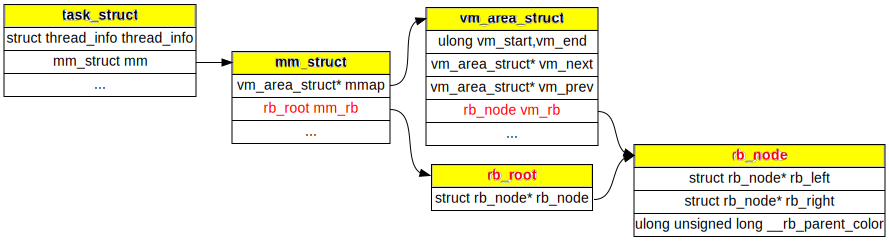
\includegraphics[width=.7\linewidth,keepaspectratio]{RBtreeInMMDesriptor.dot.colored.svg.pdf}
  \caption[RedBlackTree nella gestione degli address space in Linux]
  {Rappresentazione delle strutture usate per la gestione dello spazio degli indirizzi di un processo
			evidenziando la presenza dei RedBlack Tree}
  \decoRule \label{fig:RBtreeInMMDesriptor}
\end{figure}
Nella figura precedente è evidenziato come da un processo \vvv{p}(\verb|task_struct|) è possibile
accedere al suo \vvv{Memory Descriptor} associato (\verb|mm_struct|), contente le varie 
regioni di memoria (\verb|vm_area_struct|) relative ai vari intervalli di indirizzi 
collegati a \vvv{p}.\\
La gestione delle regioni di memoria è possibile sia mediante la strutturazione degli stessi 
in lista collegata (campi \verb|vm_next vm_prev| in \verb|vm_area_struct|),
sia mediante RedBlack tree grazie ai campi evidenziati in rosso in \ref{fig:RBtreeInMMDesriptor}
\voidLine
Dalle strutture \verb|rb_root rb_node| dei RedBlack appena mostrate è possibile notare l'assenza 
campi contenenti chiavi o puntatori a strutture nodo. 
Questo fatto è dovuto alla scelta di ottimizzare l'implementazione di queste strutture eliminando 
layers di indirezione inutili all'esecuzione delle funzionalità principali di questi alberi.
Da questa scelta degli sviluppati del kernel linux consegue la necessità di dover 
innestare le strutture \verb|rb_node| all'interno di delle strutture nodo contenti un campo chiave adeguato
ed dover implementare le funzioni di inserimento ed eliminazione nodi per ogni applicazione.
La navigazione da una struttura \verb|rb_node| alla struttura nodo che la contiene è effettuabile
semplicemente con la macro \verb|container_of| .\\%wrappata dalla macro \verb|rb_entry|

\voidLine
Le tipologie principali di RedBlack tree presenti nel kernel linux sono:	\label{linuxRBTree_}
\begin{enumerate}
	\item normali  		identificati da una radice di tipo \verb|rb_root|
	\item left-cached 	identificati da una radice di tipo \verb|rb_root_cached|
		caratterizzati dall'avere il nodo con chiave minima (più a sinistra nell'albero) salvato con un puntatore nella radice
	\item augmented		identificati da avere il suffisso \verb|_augmented| nelle operazioni associate,
		caratterizzati dall'avere salvati in ogni nodo \vvv{n} dei dati derivati dal contenuto del sotto albero con radice in \vvv{n}.\\
		Con questo tipo di RedBlack Tree è possibile implementare un supporto efficiente alla gestione di range come chiavi,
		e.g. Interval Tree \cite{rbtreeRst}
	\item latched		identificati dalle strutture radice e nodo rispettivamente \\ \verb|latch_tree_root latch_tree_node|
		utili a supportare proprietà di consistenza in esecuzioni concorrenti lock-less,
		mediante la tecnica basata su multiple versioni dei dati \emph{latch}
	%The latch technique is a multiversion concurrency control method that allows queries during non-atomic modifications. If you can guarantee queries never interrupt the modification – e.g. the concurrency is strictly between CPUs – you most likely do not need this.
	%Where the traditional RCU/lockless data structures rely on atomic modifications to ensure queries observe either the old or the new state the latch allows the same for non-atomic updates. The trade-off is doubling the cost of storage; we have to maintain two copies of the entire data structure.
\end{enumerate}

\subsection{Porting in UserSpace} 
Ho effettuato il porting in UserSpace dei primi due tipi di RedBlack tree del kernel linux 5.10.27 menzionati precedentemente 
ed ho reso disponibile il lavoro ad altri usi nel mio repository \url{https://github.com/andreadiiorio/redblackTree_linux_userspace}.
\voidLine
Per effettuare il porting delle funzioni necessarie al prodotto simbolico con RedBlack Tree è stato necessario 
rimpiazzare varie dipendenze definite in altri moduli del kernel linux come 
le macro \verb|container_of READ_ONCE WRITE_ONCE| \dots  o le funzioni di (de)allocazione
con soluzioni alternative in userspace.\\Sono state inoltre rimosse le versioni RCU delle operazioni sui RedBlack Tree per questioni di semplicità. 
\voidLine
Per supportare la fase simbolica per l'operazione di SpMM è stata realizzata una seconda versione minimalizzata del porting,
senza le funzioni non indispensabili al prodotto.\\

%Per supportare efficacemente questo ho usato il seguente approccio basato su opzioni di compilazione e linking per 
%individuare funzioni non utilizzate.\\
%\begin{lstlisting}[language=Makefile]
%DISCARDED_FUNCS_LOG="discardedFuncs.list"
%getUnusedFuncs_ld_mapfile: \$(srcAddOnly)
%	rm -f *.o	
%	$(CC) -c $(filter-out %.h ,$^) $(CFLAGS) \
%	  -ffunction-sections -fdata-sections -fno-inline-small-functions -O0
%	$(CC) -Wl,--gc-sections *.o -Wl,-Map=mapfile
%	echo "KEEP ONLY DISCARDED SECTION OF MAPFILE" && sleep 2
%	vi mapfile
%	echo "Grepping unused functions from the whole mapfile in $(DISCARDED_FUNCS_LOG) (you may want to use this command just on the discarded section)"
%	grep  "text\." mapfile | awk '{print $$1}' | awk -F'\.' '{print $$3}' | tee $(DISCARDED_FUNCS_LOG) 
%	echo  "grepping discarded functions line numbers -> only first occurrence likelly to be the definition"
%	cat $(DISCARDED_FUNCS_LOG) | xargs -n 1 -I% sh -c 'grep -m 1 -Rn % \$(srcAddOnly) | head -1' | tee \$(DISCARDED_FUNCS_LOG).grep
%\end{lstlisting}
%La precedente regola Makefile consente di elencare alcune funzioni non usate nel codice compilato
%all'interno della tabbella di linking salvata in un file denominato nel frammento di precedente \vvv{mapfile}.\\
%
%%-ffunction-section:	ogni funzione/data item deve andare in una sezione dedicata
%%-Map: salva in \vvv{mapfile} una tabbella con informazioni di linking come il mapping in memoria di file oggetto e simboli

\section{Uso Bitmaps per inserimento efficiente di indici} \label{chSpMMAux:bitmapInsert}
Per supportare l'inserimento efficiente di indici senza ripetizioni,
in alcune versioni del prodotto simbolico descritte in \ref{chSpMMSymb:bitmapsUse} e nel gestire gl'indici di colonna 
negli accumulatori densi calcolati durante le moltiplicazioni scalari ho adottato
una struttura di ricerca basata su un insieme di bitmaps.\\
La struttura contiene una zona di memoria in cui ogni bit può rappresentare la presenza di un indice specifico
se è posto ad \vvv{1}.
\voidLine
%GMP quote
L'approccio usato è in qualche modo correlato all'idea sfruttata in \cite{GMP},
ovvero di supportare una variabile di dimensione arbitraria (in questo caso il numero massimo di indici inseribili)
con molteplici variabili, \emph{limb}, di una dimensione supportata dall'archittettura target.\\
\begin{lstlisting}
typedef unsigned __int128	uint128;
#if SPVECT_IDX_BITWISE == TRUE
	#ifndef LIMB_T
		#define LIMB_T uint128
	#endif
	typedef LIMB_T limb_t;
	typedef limb_t* nnz_idxs_flags_t;
	#define LIMB_SIZE_BIT ( sizeof(limb_t) * 8 )
#else //nnz idxs ar flags in a byte arry
	typedef uchar* nnz_idxs_flags_t;
#endif
...
typedef struct{                //smart index keeping in a dense map
	idx_t	len;               //num of nnz idx accumulated
	/* nnz index presence packing, implict space enough for all possible indexes*/
	nnz_idxs_flags_t idxsMap;
	uint idxsMapN;             //either num of limbs or len of char flag array
} SPVECT_IDX_DENSE_MAP;
\end{lstlisting}
Nel frammento di codice precedente è riportata la struttura \verb|SPVECT_IDX_DENSE_MAP|, che supporta
il generico inserimento di indici in un area di memoria accessibile con \vvv{idxsMapN}, 
tenendone traccia del numero senza ripetizioni in \vvv{len}.\\
La macro di configurazione a riga 2 \verb|SPVECT_IDX_BITWISE| determina se la struttura sarà realizzata
mediante bitmaps o array di char.\\
Nel caso in oggetto di analisi, il tipo definito \verb|nnz_idxs_flags_t| conterrà l'indirizzo
di un array di bitmaps o \emph{limb}.
\voidLine
La dimensione di ogni \emph{limb} è definibile nel tipo \verb|limb_t| a tempo di compilazione a riga 3, 
configurato di default all'estensione C di GCC per interi a 128bit con il tipo \verb|__int128| \cite{gcc10.1}.\\
%Insert details
Considerando un dimensionamento della struttura per contenere $N$ indici, con \emph{limb} di dimensione $b$ bits
saranno necessari $\left\lceil \frac{N}{b}  \right\rceil$ \emph{limb}.
L'inserimento dell'indice $i$ è effettuato mediante un'operazione di OR logico di un \vvv{1} nell'
$\left\lceil \frac{i}{b}  \right\rceil$-esimo \emph{limb} nel $i ~mod~ b$-esimo bit.\\
Per supportare efficientemente il mantenimento del numero di indici inseriti, ad ogni inserimento 
viene associata una preventiva operazione di controllo se il bit target è già posto ad 1,
in caso contrario avviene l'operazione OR e viene incrementato un contatore.\\
\begin{lstlisting}
static inline int spVect_idx_in(idx_t idx, SPVECT_IDX_DENSE_MAP* idxsMapAcc){
	uint limbID 	= idx / LIMB_SIZE_BIT; //idx's limb id
	uint limbIdxID	= idx % LIMB_SIZE_BIT; //idx's pos in limb
	limb_t idxPos   = ((limb_t) 1) << limbIdxID;
	if (!( idxsMapAcc->idxsMap[limbID] & idxPos) ){
		idxsMapAcc->idxsMap [limbID] |= idxPos;
		idxsMapAcc->len++;
		return 0;
	}
	return 1;
}
\end{lstlisting}
Nel frammento di codice precedente viene implementata l'operazione di inserimento di un indice nel set di bitmaps (riga 6) 
incrementando il contantore degli indici inseriti senza duplicati a riga 7 come descritto.\\
% TODO TODO  \paragraph{Prodotto simbolico di una (partizione di) riga della matrice output con Bitmaps VS RedBlack Tree}
% È possibile affermare che nel caso di dover generare un prodotto simbolico accurato, con output limitato
% al numero di \nnz per riga \ref{chSpMMSymb:outputDetailLevel},
% l'utilizzo delle bitmap ha un costo unitario per inserimento invece che logaritmico sul numero di nodi inseriti.\\
% Nel caso di dover generare la versione \verbOutIdxs_| del operazione in oggetto, è necessario tenere traccia

\section{Configurazione chunksize dello scheduling dynamic OpenMP} \label{chSpMMAux:dynChunkFairAdapting}
Usare uno scheduling di tipo Dynamic in un ciclo parallelizzato con OpenMP 
può essere molto utile nel caso di problemi in cui il lavoro assegnabile ai thread ha una grande variabilità.\\
Nelle operazioni di SpMM e Sp3MM, la variabilità del lavoro è dovuta 
al pattern di sparsità dei \nnz nelle matrici di input.
%vs static: vantaggio per lavoro variabile
\voidLine
%false cache sharing
Lo scheduling Dynamic assegna un chunksize di dimensione pari ad 1 di default, 
il che può facilmente causare problemi di \emph{false cache sharing}.
%\paragraph{False Cache Sharing con chunksize di default di scheduling Dynamic}
Ovvero situazioni in cui il lavoro assegnato ad un thread \vvv{a} modifica una piccola area di memoria
troppo vicina a quello di un altro thread \vvv{b}, 
al punto in cui le due aree mappano su linee di cache con una intersezione. 
In questo caso, una modifica del thread \vvv{a} sulla sua area di memoria invalida la 
copia della linea di cache intersezionata del thread \vvv{b}, causando un pessimo uso della memoria.
\voidLine
%CORE
Lo scheduling Dynamic in confronto allo scheduling static di OpenMP, al costo di un overhead di istanziazzione e gestione maggiore,
consente ad un thread che ha terminato il proprio lavoro di prenderne altro da una coda acceduta concorrentemente,
evitando di restare bloccato in attesa sprecando risorse computazionali.\\
Conseguentemente, per il problema in analisi usare uno scheduling Dynamic con chunksize che sia un compromesso tra un valore piccolo e un 
chunksize statico, dato della divisione del numero di iterazioni per il numero di thread,
può dare dei benefici prestazionali.\\
Per realizzare questa funzionalità ho realizzato una funzione che adatta dinamicamente 
il chunksize di un ciclo parallelizzato ad $\frac{\#\text{iterazioni}}{\# \text{thread} \cdot \text{FAIR\_CHUNKS\_FOLDING}}$
dove \verb|FAIR_CHUNKS_FOLDING| è una macro configurabile a tempo di compilazione.\\

\section{Configurazione automatica della griglia di partizionamento del lavoro}	\label{chSpMMAux:ompGrid}
Nelle implementazioni parallele di SpMM descritte in \ref{Chapter3} è prevista una suddivisione della computazione del risultato
tra i vari thread mediante sia il chunksize configurato in openMP, sia tramite una griglia di partizionamento del lavoro.\\
Il chunksize dello scheduling openMP configurato determina quante iterazioni di un ciclo parallelizzato affidare ad un thread
ed è configurato automaticamente in base al tipo di scheduling come descritto precedentemente in \ref{chSpMMAux:dynChunkFairAdapting}.\\
La griglia di partizionamento consiste in una suddivisione del risultato da calcolare in blocchi 1D o 2D.
\voidLine
Nel caso di implementazioni monodimensionali è possibile suddividere la computazione in blocchi di righe sia automaticamente 
mediante il chunksize di openMP, sia mediante un pre-partizionamento delle righe in blocchi all'interno del ciclo parallelizzato.
L'approccio usato in quest'ultimo caso è quello di suddividere le righe del risultato in blocchi di dimensione simile,
in numero pari \\ \verb|SPMM_1DBLOCKS_THREAD_ITERATION_FACTOR| volte il numero di thread configurato per il calcolo.\\
\voidLine
Nel caso di implementazioni bidimensionali di SpMM è necessario strutturare il calcolo del risultato in blocchi 2D, corrispondenti
a una suddivisione delle righe di A e delle colonne di B rispettivamente in \vvv{gridRows}x\vvv{gridCols} blocchi.\\
Mediante le seguenti euristiche, la determinazione della griglia di partizionamento è stata resa configurabile 
in base al numero di thread configurato per l'esecuzione:\\
\begin{itemize}
	\item	automaticamente in una griglia di blocchi determinata mediante un porting che ho realizzato 
			della funzione \verb|MPI_Dims_create| da OpenMPI
	\item	a partire da una suddivisione delle colonne di B 
			da cui derivare un partizionamento delle righe di A pari a $\left\lceil \frac{numThread}{gridCols}  \right\rceil$
	\item	un partizionamento fisso, configurabile manulamente a tempo di compilazione con le macro
			\verb|FIXED_2D_PARTITIONING_ROWS FIXED_2D_PARTITIONING_COLS|
\end{itemize}
\subsection{porting funzione MPI\_Dims\_create da OpenMPI}	\label{ompiDimsCreate}
Al fine di supportare una suddivisione del lavoro di SpMM per il numero di thread $nThread$ configurato
in una griglia di partizionamento 2D, il più quadrata possibile, ho realizzato un porting della 
funzione \verb|MPI_Dims_create| da OpenMPI.
\voidLine
Nel contesto della programmazione a memoria distribuita, 
la funzione \\ \verb|MPI_Dims_create| consente di determinare una suddivisone bilanciata di un numero di processi in una topologia 
cartesiana n-dimensionale da utilizzare durante il calcolo \cite{mpi}.\\
Nella determinazione della griglia di partizionamento per implementazioni bidimensionali di SpMM ho usato 
\verb|MPI_Dims_create| per suddividere il numero di thread configurato nei parametri \verb|gridRows gridCols|.
Nel caso di utilizzare un numero di thread primo è impossibile ottenere una suddivisione esatta non monodimensionale,
ma ho gestito questi casi suddividendo $nThread+1$ in luogo di $nThread$, 
così da poter assegnare almeno un iterazione ad ogni thread.\\


\section{Assegnamento dinamico di memoria ai thread \emph{fence-less}} \label{chSpMMAux:atomicSegAssign}
Nel caso di effettuare la \emph{sparsificazione} di un accumulatore denso 
durante il prodotto numerico di SpMM, descritta precedentemente in \ref{chSpMMNum:sparsify},
in assenza di informazioni sulla quantità di memoria necessaria ad ogni thread, 
è necessario assegnare dinamicamente partizioni di memoria (pre allocata), in maniera concorrente.
\voidLine
Un approccio semplice allo scopo è quello di utilizzare una qualche primitiva di sincronizzazione
, funzionalmente simile ad un \emph{lock}, per proteggere una sezione critica in cui
si annota che il thread corrente si è riservato un segmento del blocco di memoria condiviso.\\
%TODO TODO CHECK TRIVIAL LOCK APROCH:	USELESS FENCE
Tuttavia, quest'approccio potrebbe introdurre istruzioni di \vvv{fence} intorno alla sezione critica,
causando una serializzazione deli accessi di memoria effettuati fin a quel momento.\\
%ATOMIC BUILT IN APPROCH
Per ridurre al minimo l'overhead di sincronizzazione per realizzare questa assegnazione
ho usato due approcci equivalenti.
%per effettuare una somma atomica di una variabile, salvandone il contenuto precedente all'incremento.\\

\subsection[Uso built-in atomiche di GCC]
{Riservazione concorrente di memoria mediante built-in atomiche di GCC}
Un approccio diretto al problema è quello di usare la built-in atomica offerta da gcc
\verb|type __atomic_fetch_add (type *ptr, type val, int memorder)|
su una variabile atomica, contente l'indice dell'ultimo elemento assegnato del blocco di memoria condiviso ad un thread.\\
%Il thread che necessita di uno spazio $s$ dalla zona di memoria pre allocata, ....
\begin{lstlisting}
sparsifyStartV = __atomic_fetch_add(&(acc->lastAssigned),nnz,__ATOMIC_ACQ_REL); 
\end{lstlisting}
Nel frammento di codice precedente, relativo alla sparsificazione di un accumulatore denso,
viene mantenuto l'indice iniziale dello spazio di memoria condiviso non assegnato.\\
Ogni thread riserverà uno spazio di memoria mediante l'incremento atomico 
del numero di elementi da salvare (\vvv{nnz}) sulla variabile \vvv{lastAssigned}.\\
L'indirizzo iniziale del blocco di memoria riservato al thread sarà il valore precedente all'incremento
di \vvv{lastAssigned} ed è salvato nella variabile \vvv{sparsifyStartV}.
\voidLine
L'uso di questa primitiva è da associare ad un modello di ordine di memoria \vvv{memorder}.\\
Per l'operazione da realizzare dovrebbe essere sufficiente il modello \\ \verb|__ATOMIC_ACQ_REL|,
che sostanzialmente crea una relazione di tipo \emph{happens-before} tra le operazioni di 
\emph{acquire} e \emph{release} sulla variabile atomica  \cite{isoc11,gcc10.1}.\\

\subsection[Uso clausola \vvv{capture} di OpenMP]
{Riservazione concorrente di memoria mediante OpenMP}
Un approccio del tutto equivalente è usare la clausola \vvv{capture} al construttuto \vvv{atomic} di openMP.\\
Segue una porzione di codice per realizzare la funzionalità in analisi.
\begin{lstlisting}
#pragma omp atomic capture
{   //fetch and add like 
    sparsifyStartV = acc->lastAssigned;
    acc->lastAssigned += nnz;
}
\end{lstlisting}

\subsection{Confronto implementazione operazione atomica}
Per confrontare le soluzioni, valutando anche altri modelli di memoria,
ho effettuato un dissasemblamento del codice compilato con gcc 8.5.0.\\
\begin{lstlisting}[language={[x86masm]Assembler}]
sparsifyStartV = __atomic_fetch_add(&(acc->lastAssigned),nnz,__ATOMIC_SEQ_CST); 
mov		-0x18(%rbp),%rax
add		$0x18,%rax
mov		-0x8(%rbp),%edx
lock 	xadd %edx,(%rax)
mov		%edx,-0xc(%rbp)

sparsifyStartV = __atomic_fetch_add(&(acc->lastAssigned),nnz,__ATOMIC_ACQ_REL); 
mov		-0x18(%rbp),%rax
add		$0x18,%rax
mov		-0x8(%rbp),%edx
lock	xadd %edx,(%rax)
mov		%edx,-0xc(%rbp)

#pragma omp atomic capture
{   //fetch and add like .... 
	sparsifyStartV = acc->lastAssigned;
	acc->lastAssigned += nnz;
}
mov		-0x18(%rbp),%rax
add		$0x18,%rax
mov		-0x8(%rbp),%edx
lock	xadd %edx,(%rax)
mov		%edx,-0xc(%rbp) 
\end{lstlisting}
%$	%TODO uncomment to avoid wrong highlighting in vim
Nel frammento di codice precedente vengono confrontati il dissasemblamento del codice
configurato ad usare rispettivamente: 
\begin{itemize}
	\item la \verb|__atomic_fetch_add| con modello di consistenza \verb|__ATOMIC_SEQ_CST|, 
	  che dovrebbe offrire un ordinamento totale delle operazioni,
	\item la \verb|__atomic_fetch_add| con modello di consistenza \verb|__ATOMIC_ACQ_REL|
	\item il costrutto openMP \vvv{atomic} precedentemente visto.\\
\end{itemize}
È possibile notare come il codice Assembly prodotto sia sempre lo stesso,
basato sull'uso di un'operazione di Exchange and Add con prefisso \vvv{LOCK}.\\
L'atomicità dell'implementazione è provata dalla presenza di questo prefisso,
che come la documentazione intel riporta, 
%LOCK prefix intel man 2
consente al processore corrente di avere uso esclusivo di ogni memoria condivisa \cite{intelDevMan2}.\\


\section{Partizionamento bidimensionale di una matrice CSR}	\label{chSpMMAux:CSR2DPARTI}
Per effettuare un partizionamento 2D di una matrice CSR è sufficiente
dividere le colonne in gruppi ed accederne le righe.
Dato che il vettore IRP della rappresentazione CSR permette di accederene facilmente le righe,
avendo la conoscenza addizionale dei limiti di ogni partizione di colonne è possibile accedere blocchi bidimensionali
della matrice.\\
Una rappresentazione grafica dell'operazione è raffigurata nell'immagine seguente.\\
\begin{figure}[H]
  \centering \includegraphics[width=.7\linewidth,keepaspectratio]{csrTilingCSR_only.svg.pdf} 
  \caption[partizionamento 2D CSR]
  {Rappresentazione grafica di un partizionamento 2D di una matrice CSR, \cite{adaptiveTilingSpMM}}
  \decoRule \label{fig:csrTilingCSR_only}
\end{figure}

La suddivisione delle colonne di una matrice CSR, necessaria per il suo partizionamento 2D, 
può essere effettuata \emph{in loco} o mediante sotto matrici CSR separate con una struttura di offest di supporto.

Nel seguito saranno descritte due soluzione che ho realizzato per effettuare l'operazione in oggetto.\\

\subsection{Partizionamento colonne in loco mediante offsets di supporto} 
\label{chSpMMAux:csrColPartitioning}
Per accedere in loco una matrice CSR $M\times N$ in blocchi bidimensionali di $\frac{M}{gridRows}\times\frac{N}{gridCols}$, 
ho realizzato un supporto alla generazione di una matrice di offset $M\times gridCols$, dove l'elemento
$i,j$ è relativo all'inizio della $j$-esima partizione di colonne della $i$-esima riga.\\
\begin{lstlisting}
///OFFSETS COMPUTE FOR COL GROUPS -> O( A.NZ )
for (ulong r=0, j=0;     r<A->M;     j=A->IRP[++r]-OFF_F){
    offsets[ IDX2D(r,0,gridCols) ] = j;  //row's first gc start is costrained
    for (ulong gc=1,gcStartCol;  gc<gridCols;  gc++){
        gcStartCol = UNIF_REMINDER_DISTRI_STARTIDX(gc,_colBlock,_colBlockRem);
        //goto GroupCols start entry,keeping A's nnz entries navigation (idx j)
        while ( j < A->IRP[r+1]-OFF_F &&  A->JA[j]-OFF_F < gcStartCol )  j++;
        offsets[ IDX2D(r,gc,gridCols) ] = j;  //row's gc group startIdx
    }
}
\end{lstlisting}
Nel frammento di codice precedente è possibile vedere come la matrice da partizionare è scansionata
linearmente, salvandone l'indice di colonna corrente ogni volta che 
viene raggiunto o superato l'inizio di un gruppo di colonne.\\

\subsection{Partizionamento colonne mediante sotto-matrici dedicate} \label{chSpMMAux:csrColPartitioningAllocatd}
Un approccio alternativo al precedente è quello di separare i gruppi di colonne della matrice da 
partizionare in sotto matrici separate.
Successivamente è possibile accedere un blocco 2D della matrice originaria partizionando 
le righe (indirizzandole con IRP) di ogni sotto matrice ottenuta.\\
Ho realizzato due implementazioni di quest'approccio,
uno basato sull'uso della struttura ausiliara vista nella sottosezione precedente, 
ed un'altra basata su una scansione diretta della matrice, simile al caso precedente.\\ 

\begin{lstlisting}
for (ulong r=0, j=0;     r<A->M;     j=A->IRP[++r]-OFF_F){
    //navigate column groups inside current row
    for (ulong gc=0,gcEndCol=0,i;  gc<gridCols ;  gc++,j+=i){
        i = 0;  //@i=len current subpartition of row @r to copy
        colPart = colParts + gc;
        colPart->IRP[r] = colPartsLens[gc];	
        gcEndCol += UNIF_REMINDER_DISTRI(gc,_colBlock,_colBlockRem);
        //goto next GroupCols,keeping A's nnz entries navigation ( index j+i )
        while ( j+i < A->IRP[r+1]-OFF_F && A->JA[j+i]-OFF_F < gcEndCol ) i++;
        memcpy(colPart->AS+colPart->IRP[r], A->AS+j, i*sizeof(*A->AS));
        memcpy(colPart->JA+colPart->IRP[r], A->JA+j, i*sizeof(*A->JA));
        
        colPartsLens[gc] += i;
		#ifdef ROWLENS
        colPart->RL[r] = i;
		#endif
    }
}
\end{lstlisting}
Nel frammento di codice precedente è possibile vedere come scansionando la matrice da partizionare,
si associ all'indice corrente l'inizio della partizione di colonne da riempirea(\vvv{j})
e la dimensione (\vvv{i}) della sotto riga attuale.%nella partizione di colonne.
Con queste informazioni è possibile effettuare una \vvv{memcpy} dei \nnz relativi 
\vvv{gc}-esima partizione della \vvv{r}-esima riga della matrice (righe 10-11),
dopo che l'indice di scanzionamento corrente della matrice \vvv{j+i} sia arrivato alla 
fine della sotto riga da copiare.\\

\subsection{Confronto teorico delle due soluzioni}
\begin{itemize}
	\item
	L'approccio basato sulla generazione di sottomatrici per ogni partizione di colonna 
	soffre di un overhead di inizializzazione superiore all'altro dato che 
	oltre che scansionare la matrice per identificarne blocchi di colonne, è necessario effettuarne
	copie in altre zone di memoria.\\
	\item 
	L'approccio basato sulla struttura di indicizzazione ausiliaria applicato alla realizzazione
	del prodotto numerico con partizionamento 2D del lavoro, soffre di una possibile penalità di memoria
	nell'accedere righe consecutive di una stessa partizione, dato che i \nnz relativi non sono 
	contigui in memoria.
\end{itemize}

\section{Verfica correttezza delle implementazioni}
Tutte le implementazioni parallele realizzate per Sp3MM sono state verificate 
mediante un confronto con una matrice risultante ottenuta esternamente o
da una implementazione seriale di riferimento.
In entrambi i casi, il confronto è considerato positivo se c'è una uguaglianza esatta 
tra le dimensioni delle matrici e gli indici degli elementi \nnz (il componente \vvv{JA} del formato CSR)
e se i valori floating point delle matrici sono uguali a meno di una soglia di tolleranza (configarata con $7~10^{-4}$.\\
È importante sottolineare la necessità di effettuare il confronto tra valori \nnz delle matrici con una soglia,
%dato che le rappresentazioni floating-point per i numeri reali sono soggetti ad errori di approssimazione, 
dato che le operazioni tra rappresentazioni floating-point sono soggette ad errori di approssimazione che possono portare 
a risultati diversi in base al sequenziamento delle operazioni effettuate (non prevedibile in una implementazione parallela)
\cite{goldmanFP}

\subsection{implementazione seriale di riferiemento}	\label{implSerialeRiferimento}
L'implementazione seriale di riferimento è stata realizzata con una coppia di operazioni di SpMM
realizzate con un approccio \rowbyrow, in modo molto simile alle implementazioni monodimensionali descritte in \ref{chSpMMNum:part1DGroup}.
A differenza della controparte parallela, l'implementazione seriale gode della grande facilitazione 
di poter scrivere le righe della matrice risultante direttamente nell'output dell'operazione senza una fase simbolica precedente,
data la possibilità di accumulare le lunghezze delle righe calcolate precedentemente alla corrente.\\
\voidLine
Per validare gli output dell'implementazione seriale per alcuni input di piccola dimensione,
è stato effettuato un confronto con una implementazione di riferimento per matrici dense: \vvv{CBLAS} in \url{http://www.netlib.org/blas/},
in seguito ad una trasformazione delle matrici da un formato sparso ad uno denso.\\

\section{Distribuzione uniforme del lavoro tra i thread}	\label{chSpMMAux:UNIF_REMINDER_DISTRI}
Distribuire uniformemente il carico di lavoro tra i thread è un'operazione importante,
che consente di minimizzare il divario tra i tempi di completamento dei vari thread 
e conseguentemente anche il tempo di esecuzione parallelo
(dal momento che è definito con l'istante di terminazione dell'ultimo thread).\\

Algoritmi paralleli basati su strutture sparse sono spesso accumunati da 
un'impossibilità di determinare efficientemente il carico di lavoro di effettivo
relativo ad una partizione dell'input.
Nonostante ciò, può essere utile distribuire il più uniformente possibile ogni partizione 
di dati e iterazioni tra i thread .\\%in assenza di informazioni che consentano di effettuare un partizio
Considerando un input di dimensione $n$ da suddividere tra $t$ threads, avendo\\
$div=\left\lfloor \frac{n}{t}  \right\rfloor ~ rem=n ~mod ~t$,
l'approccio seguito per minimizzare il divario delle partizioni assegnate %a vari thread
è realizzato dalla seguente macro:\\
\verb|#define UNIF_REMINDER_DISTRI(i,div,rem) ((div)+((i)<(rem)?1:0 ))|
dove viene redistribuito il resto della divisione $rem$ tra i thread.\\
			%auxiliary solutions (referenced from behind)
\chapter{Analisi delle performance delle implementazioni realizate}
\label{ChPerf}

Ho effettuato un analisi delle performance ottenute nelle varie implementazioni 
realizzate per Sp3MM con un insieme eterogeno di matrici di input.\\
Le prestazioni confrontate sono ottenute da valori mediati su 40 ripetizioni
dalle varie implementazioni e configurazioni realizzate per Sp3MM descritte precedentemente.\\
I dati sono stati raccolti mediante un programma di test ( \verb|Sp3MM_test.c| ) automatizzando
l'esecuzione di tutte le implementazioni realizzate dato un set di matrici di input.
I log del programma di test sono stati parsati ed analizzati mediante la libreria di analisi Pandas \cite{pandasMan}.\\
Tutti i test sono stati effettuati sul server dell'Ateneo, caratterizato dai seguenti parametri:
\begin{itemize}
	\item	 OS:	CentOS Stream 8
	\item	CPU:	Intel Xeon Silver 4210 2.20 GHz 40 core
	\item	RAM:	64GB
\end{itemize}

\section{Matrici di input utilizzate} \label{chPerf:inputs}
Il problema originario risolto è un sistema lineare ottenuto da 
una discretizzazione alle differenze finite 
di una PDE di secondo ordine,
utilizzando una griglia regolare e le condizioni al contorno di Dirichlet.\\ %(corrispondente al programma di test di PSBLAS).
Le matrici sparse utilizzate nei test
sono relative ai tripli prodotti di Galerkin in due configurazioni
di generazione degli aggregati in AMG4PSBLAS:
\emph{VanekBrezina} e \emph{Matching}, entrambe con e senza un operazione di smoothing associata.\\
Le caratteristiche del problema di partenza da cui sono derivate i gruppi di matrici,
comportano un pattern di sparsità degli elementi non zero di tipo diagonale 
come è visibile nelle figure seguenti.\\

\begin{figure}[H]
  \centering \includegraphics[width=\linewidth,keepaspectratio]{sparseMatrices/matchingMediumSmoothed_UnSmoothed.png}
  \caption[pattern dei non zeri nelle matrici Matching]
  {rappresentazione degli elementi \nnz di matrici ottenute con il metodo Matching, con opzione smoothed a sinistra, unsmoothed a destra}
  \decoRule \label{fig:sparseMatrix}
\end{figure}
\begin{figure}[H]
  \centering \includegraphics[width=\linewidth,keepaspectratio]{sparseMatrices/vanekBrezina_MediumSmoothed_UnSmoothed.png}
  \caption[pattern dei non zeri nelle matrici VanekBrezina]
  {rappresentazione degli elementi \nnz di matrici ottenute con il metodo VanekBrezina, con opzione smoothed a sinistra, unsmoothed a destra}
  \decoRule \label{fig:sparseMatrix1}
\end{figure}
\label{inputClasses}
Data l'eterogeneità degl'input utilizzati, 
ho raggruppato le matrici di test in quattro gruppi in base alla tecnica di generazione degli aggregati %(ovvero le matrici R e P nel prodotto di Galerkin)
e l'uso dello dello smoothing.\\
I gruppi di input utilizzati sono quindi: 
\begin{enumerate}
	\item VanekBrezina,Smoothed
	\item VanekBrezina,Unsmoothed
	\item Matching,Smoothed
	\item Matching,Unsmoothed
\end{enumerate}

\section{Configurazioni considerate}
Tra i svariati parametri configurabili a compile-time o a run-time, è stata effettuata 
un analisi di tutte le implementazioni realizzate variando:
\newcounter{queriesCounter}
\begin{enumerate}
	\item	il tipo di assegnamento ai thread dello spazio intermedio in implementazioni basate su UpperBound 
	\item	la dimensione delle bitmap utilizzate in alcune implementazioni del prodotto simbolico %(descritte in \refbf{chSpMMSymb:structFlagSet})
	\item	il numero di thread da utilizzare 
	\item	il tipo di scheduling openMP: static o dynamic adattato (descritto in \refbf{chSpMMAux:dynChunkFairAdapting})
	\setcounter{queriesCounter}{\value{enumi}}
\end{enumerate}
Inoltre, sono state determinate le performance:
\begin{enumerate}
	\setcounter{queriesCounter}{\value{enumi}}
	\item	di ogni implementazione, con configurazione ottimale, per ogni categoria di input (descritte in \refbf{inputClasses})
	\item	della migliore implementazione per ogni input, confrontadole con le performance ottenute con un implementazione seriale di riferimento
\end{enumerate}
Altri parametri, come la griglia di partizionamento utilizzata, sono determinati automaticamente in base al numero di thread configurato,
come descritto in \refbf{chSpMMAux:ompGrid}.
In particolare per implementazioni bidimensionali, la griglia di partizionamento impiegata è stata determinata con l'approccio
basato sulla funzione \verb|MPI_Dims_create|, descritto in \refbf{ompiDimsCreate}.\\
\begin{figure}[H]
  \centering 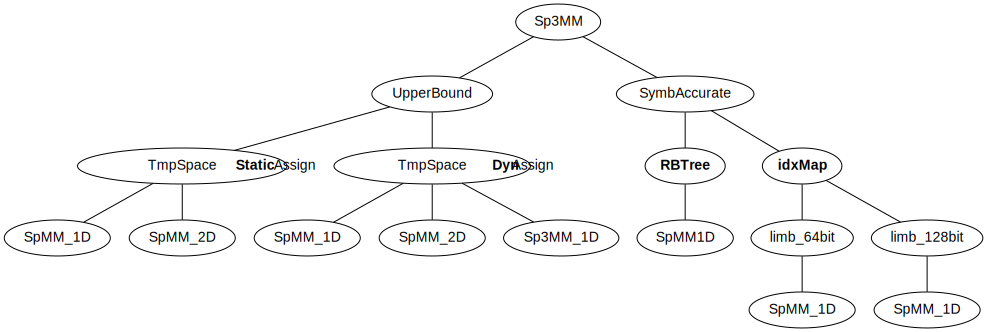
\includegraphics[width=\linewidth,keepaspectratio]{Sp3MM_treeMinimal.dot.txt.svg.pdf}
  \caption[implementazioni Sp3MM realizzate]
  {Diagramma riassuntivo delle varie configurazioni delle implementazione realizzate considerate nei test con scheduling openMP static e dynamic adattato}
  \decoRule \label{fig:q1}
\end{figure}
\voidLine
Tutti i test nel seguito ad eccezione di quelli menzionati nella sezione \refbf{chPerf:multiThread}, sono stati effettuati 
con il numero massimo di thread possibili, ovvero 40 sull'ambiente di esecuzione utilizzato.\\


\section{Determinazione della migliore configurazione}	\label{bestConf}
Nel seguito viene determinata la migliore configurazione, mediando le performance misurate nelle implementazioni relative alle configurazioni considerate,
su tutti gli input disponibili e tutti i tipi di scheduling openMP

\subsection[Migliore assegnamento di spazio intermedio per\\implementazioni UpperBound]
{Migliore assegnamento di spazio intermedio per implementazioni UpperBound}
Come analizzato in \refbf{chSpMMSymb:UB_VS_SYMBACC}, implementazioni parallele di SpMM basate su una fase simbolica di tipo UpperBound,
necessitano inevitabilmente di uno spazio temporaneo per i risultati intermedi, 
che ho pre-allocato al blocco di esecuzione parallelo 
ed assegnato ai thread in modo statico o dinamico, 
come descritto in \refbf{chSpMMNum:preSplitAS_JA_tmp} ed approfondito in \refbf{chSpMMAux:atomicSegAssign}.\\

\begin{figure}[H]
  \centering 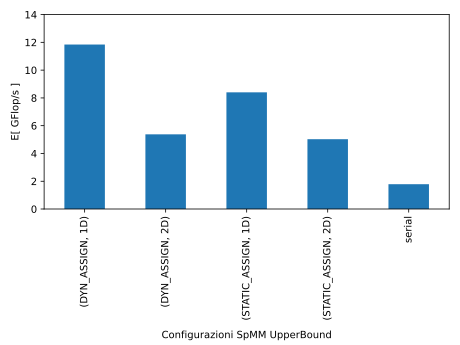
\includegraphics[width=\linewidth,keepaspectratio]{graphs/q1.svg.pdf}
  \caption[UB: confronto assegnamento spazio temporaneo]
  {Confronto tra le perfomance medie delle implementazioni UpperBound di SpMM, su tutti gli input considerati, in base a
		tipo di assegnamento dello spazio intermedio ai thread (statico o dinamico) e al tipo di implementazione usata 
		( con partizionamento del lavoro 1D o 2D ) }
  \decoRule \label{fig:q1}
\end{figure}

Come è possibile vedere nella figura \refbf{fig:q1}, un assegnamento dinamico dello spazio intermedio ai thread da dei vantaggi
per implementazioni monodimensionali, mentre ha performance pressochè simili nel caso di implementazioni bidimensionali.\\

\subsection[Migliore dimensione bitmap nel prodotto simbolico accurato]
{Migliore dimensione delle bitmap per implementazioni con prodotto simbolico accurato}
La versione del prodotto simbolico accurato basata su bitmap di indici, descritta in \refbf{chSpMMSymb:structFlagSet} 
ed approfondita in \refbf{chSpMMAux:bitmapInsert}, prevede l'uso di un vettore di variabili di tipo \verb|limb_t|
di dimensione configurabile a tempo di compilazione con la macro \verb|LIMB_T|.\\

\begin{figure}[H]
  \centering 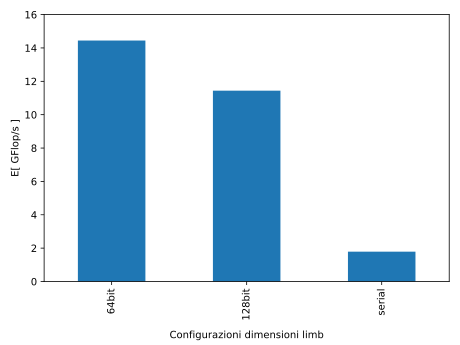
\includegraphics[width=\linewidth,keepaspectratio]{graphs/q2.svg.pdf}
  \caption[SymbAcc: miglior dimensione per le bitmaps]
  {Confronto tra le perfomance medie di Sp3MM con fase simbolica accurata mediante bitmaps di indici,
		   su tutti gli input considerati, variando la dimensione delle singole bitmap tra 64 e 128 bit}
  \decoRule \label{fig:q2}
\end{figure}
Dalla figura \refbf{fig:q2} è possibile notare come usare bitmap di 64 bit può può fornire un vantaggio prestazionale
rispetto all'uso di bitmap a 128 bit.

\section{Migliore implementazione per classe di input} \label{chPerf:q3}
Considerando la miglior configurazione determinata in \refbf{bestConf}, ho effettuato un confronto delle prestazioni medie
delle varie implementazioni di Sp3MM per ogni classe di input disponibile ( descritte precedentemnte in \refbf{inputClasses} )
%\centering \includegraphics[width=\linewidth,keepaspectratio][[width=\linewidth,keepaspectratio]{q3.svg.png}
\begin{figure}[H]	
  \centering \includegraphics[width=\linewidth,keepaspectratio]{graphs/q3.svg.pdf}
  \caption[miglior implementazione per classe di input]
  {Confronto tra le perfomance medie della miglior configurazione per le implementazioni di Sp3MM per ogni classe di input}
  \label{fig:q3}
\end{figure}
Come è possibile notare dalla figura \refbf{fig:q3}, si hanno performance molto diverse in base alla classe di input considerata.
In particolare, le implementazioni su matrici di tipo \emph{Unsmoothed} soffrono di prestazione nettamente inferiori di quelle 
su matrici \emph{Smoothed}.\\
Le implemenetazioni con performance migliori variano tra le classi di input considerate, tuttavia è possibile osservare che:
\begin{itemize}		\label{chPerf:inClassPerfOss}
	\item il triplo prodotto diretto dia prestazioni migliori degli altri in tutte le classi salvo \emph{VanekBrezina,Unsmoothed}.
	\item la configurazione di scheduling openMP static sembra dare prestazioni migliori per le implementazioni bidimensionali,
		  viceversa la controparte dynamic con chunk adattati da risultati migliori per implementazioni monodimensionali e per il triplo prodotto diretto.
	\item le implementazioni monodimensionali UpperBound performano meglio di quelle bidimensionali nelle classi di input \emph{Smoothed},
		  viceversa per le classi \emph{Unsmoothed}
\end{itemize}

\section{Guadagno di performance rispetto ad una implementazione seriale} \label{chPerf:allMatrixs}
Come precedentemente analizzato le prestazioni di Sp3MM sono molto variabili in base al tipo di input, 
l'implementazione utilizzata e la configurazione applicata.\\
Per questo motivo ho deciso di misurare il vantaggio prestazionale ottenuto dalla migliore implementazione parallela 
rispetto ad una implementazione seriale di riferimento ( descritta in \refbf{implSerialeRiferimento} ).\\
\begin{figure}[H]
  \centering 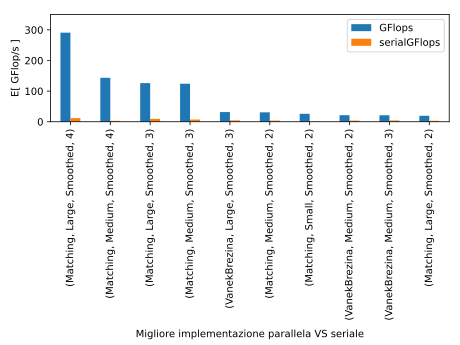
\includegraphics[width=\linewidth,keepaspectratio]{graphs/q4-b.svg.pdf}
  %\captionlistentry	FOR NO CAPTION LABEL REFERING
  \caption[Migliore implementazione parallela VS seriale - 1]
  \decoRule \label{fig:q4big}
\end{figure}
\begin{figure}[H]
  \centering 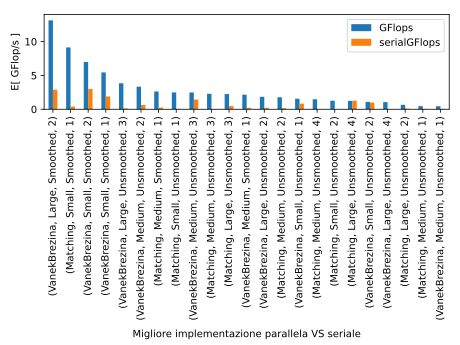
\includegraphics[width=\linewidth,keepaspectratio]{graphs/q4-s.svg.pdf}
  %\captionlistentry	FOR NO CAPTION LABEL REFERING
  \caption[Migliore implementazione parallela VS seriale - 2]
  \decoRule \label{fig:q4small}
\end{figure}
Come è possibile notare dai grafici \refbf{fig:q4big}, \refbf{fig:q4small}, le implementazioni 
parallele di Sp3MM performano meglio dell'implementazione seriale per la stragrande maggioranza dei casi,
in misura variabile in base all'input considerato.\\

\section{Performance variando il numero di thread}	\label{chPerf:multiThread}
La dimensione delle matrici di input e il loro pattern di sparsità,
potrebbe comportare che le performance migliori per Sp3MM sono ottenute con un numero di thread diverso da quello massimo possibile.\\
Per questo motivo ho effettuato un analisi delle prestazioni misurate per alcune esecuzioni di Sp3MM
al variare del numero di thread.\\
\begin{figure}[H]
  \centering 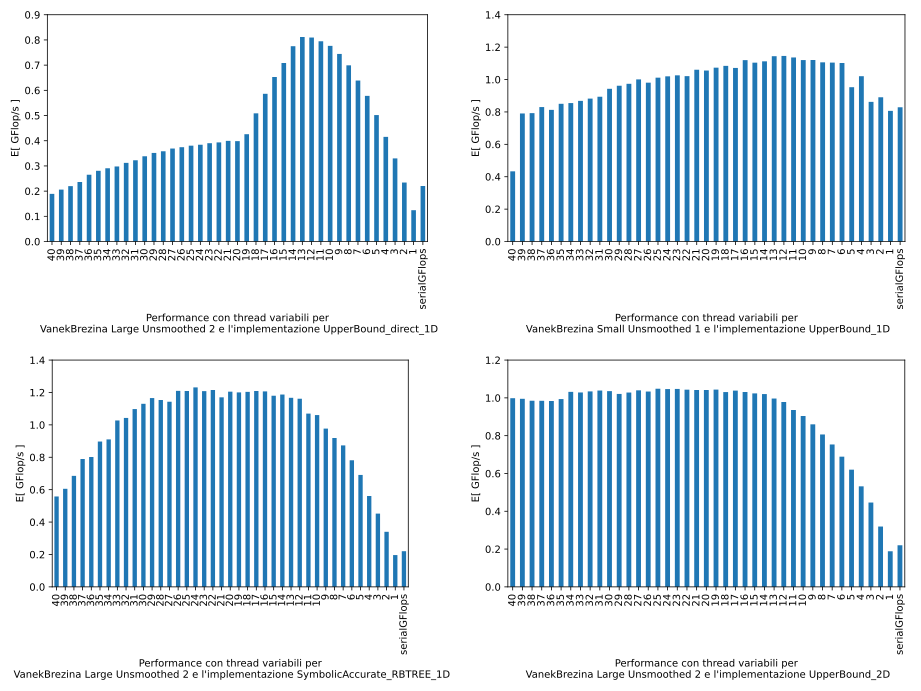
\includegraphics[width=\linewidth,keepaspectratio]{graphs/q5.svg.pdf}
  \caption[performance Sp3MM variando il numero di thread]
  {performance misurate su alcune esecuzioni di Sp3MM, variando il numero di thread impiegati}
  \decoRule \label{fig:q5}
\end{figure}
Come è possibile notare dai grafici \refbf{fig:q5}, è possibile avere un guadagno di performance 
abbassando il grado di parallelismo, in misura differente in base all'implementazione e alla matrice considerata.\\

\section{Conclusioni}
Di seguito alcune considerazioni che è possibile trarre dalle analisi delle performance effettuate.\\
%TODO gestione registri a 128 bit VS 64 ??
In generale, il pattern di sparsità dei valori \nnz delle matrici di input può causare uno sbilanciamento
nelle porzioni di lavoro assegnate ai thread in misura differente in base:
\begin{itemize}
	\item	all'approccio di divisione del lavoro usato,
	\item	alla tipologia di implementazione usata (triplo prodotto diretto o uso di una fase simolica accurata)
	\item	al tipo di scheduling openMP usato così come altre configurazioni
\end{itemize}
Uno sbilanciamento del carico di lavoro comporta un cattivo uso delle risorse computazionali, causando un peggioramento delle performance 
come come è possibile notare nell'analisi effettuate in \refbf{chPerf:q3}.\\
\voidLine
Il livello di parallelismo usato può influire molto sulle performance, come visibile nell'analisi effettuata in \refbf{chPerf:multiThread},
sia per le ragioni appena citate che per motivi legati all'overhead di schedulare un alto numero di thread
per input piccoli.
\voidLine
L'overhead complessivamente introdotto da openMP può in generale comportare un costo superiore al beneficio
ottenuto dall'esecuzione parallela per alcuni input, come visibile in pochi casi in \refbf{fig:q4small}.
Inoltre, in \refbf{fig:q5} è possibile notare uno svantaggio prestazionale in alcune esecuzioni parallele con un solo thread
rispetto all'esecuzione dell'implementazione seriale di riferimento, 
probabilmente dovuto all'overhead di inizializzazione e scheduling di openMP.\\

		%timing any confronto
%\include{Chapters/ChConclusion}			%??, ripetizione di any confronto perfs? inglobabile in perfs? 
										%configurazioni ottimali per Sp3MM + matrici da problemi diagonali
%%----------------------------------------------------------------------------------------
%%	THESIS CONTENT - APPENDICES
%%----------------------------------------------------------------------------------------
%
%\appendix % Cue to tell LaTeX that the following "chapters" are Appendices
%
%% Include the appendices of the thesis as separate files from the Appendices folder
%% Uncomment the lines as you write the Appendices
%
%\include{Appendices/AppendixA}
%%\include{Appendices/AppendixB}
%%\include{Appendices/AppendixC}
%
%%-----------------------------BIBLIOGRAPHY----------------------------------------------
%\section{Bibliografia}
\printbibliography[heading=bibintoc]

%----------------------------------------------------------------------------------------

\end{document}  
